\documentclass[a4paper,12pt]{book}
\usepackage[legalpaper, portrait, margin=0.5in]{geometry}
\usepackage[utf8]{inputenc}
\usepackage{graphicx}
\usepackage{braket}
\usepackage{dsfont}
\usepackage{amsmath}
\usepackage{mathtools}
\usepackage{cancel}
\usepackage{bbold}
\usepackage{titlepic}
\usepackage{amssymb}
\usepackage{amsthm}
\usepackage{hyperref}
\setcounter{secnumdepth}{3}
\setcounter{tocdepth}{3}


\newcommand{\limit}[2]{\underset{#1 \rightarrow #2}{\lim} \,}
\newcommand{\arrowlim}[2]{\overset{#1 \rightarrow #2}{\longrightarrow}}
\newcommand{\arrowlimtwo}[4]{\overset{\scriptsize{\begin{array}{cc}
			#1 {}&\rightarrow #2\\
			#3 &\rightarrow #4
		\end{array}}
	}{\longrightarrow}}
\newcommand{\notends}{\cancel{\longrightarrow}}
\newcommand{\Exp}[1]{e^{#1}}
\newcommand{\half}{\frac{1}{2}}
\newcommand{\fracn}[1]{\frac{1}{#1}}
\newcommand{\dertot}[2]{\frac{d #1}{d #2}}
\newcommand{\dertotk}[3]{\frac{d^{#1} #2}{d #3^{#1}}}
\newcommand{\partialder}[2]{\frac{\partial #1}{\partial #2}}
\newcommand{\derdir}{D_{\hat v}}
\newcommand{\absval}[1]{\left| #1 \right|}
\newcommand{\Arctan}[2]{\arctan \left( \frac{#1}{#2} \right)}
\newcommand{\Arccotan}[2]{\arccotan \left( \frac{#1}{#2} \right)}
\newcommand{\R}{\mathbb{R}}
\newcommand{\N}{\mathbb{N}}
\newcommand{\Q}{\mathbb{Q}}

\newcommand{\Sup}[1]{\underset{#1}{sup}}

\newcommand{\doubteq}{\overset{?}{=}}

\newcommand{\taleche}{\, : \,}
\newcommand{\spacer}{\quad ; \quad}
\newcommand{\spacecomma}{\, , \,}
\newcommand{\continue}{\nonumber \\}
\newcommand{\nextpassage}{\nonumber \\ &\downarrow \nonumber \\}


\newcommand{\gradient}[2]{\nabla #1(#2)}
\newcommand{\jacobian}[2]{\boldsymbol{J}_{#1} (#2)}
\newcommand{\hessian}[2]{\boldsymbol{H}_{#1} (#2)}
\newcommand{\genericOp}{\boldsymbol{Q}}
\newcommand{\vech}{\underline{h}}
\newcommand{\vecx}{\underline{x}}
\newcommand{\vecX}{\underline{X}}
\newcommand{\vecy}{\underline{y}}
\newcommand{\vecY}{\underline{Y}}
\newcommand{\vecz}{\underline{z}}
\newcommand{\vecZ}{\underline{Z}}
\newcommand{\veczero}{\underline{0}}
\newcommand{\vecp}{\underline{p}}
\newcommand{\vecP}{\underline{P}}
\newcommand{\vecf}{\underline{f}}
\newcommand{\vecF}{\underline{F}}
\newcommand{\vecg}{\underline{g}}
\newcommand{\vecq}{\underline{q}}
\newcommand{\vecxi}{\underline{\xi}}
\newcommand{\matrixTwoTwo}[4]{\left(
	\begin{array}{ccc}
		#1 & #2 \\
		#3 & #4
	\end{array}
	\right)}
\newcommand{\matrixThreeThree}[9]{\left(
	\begin{array}{ccc}
		#1 & #2 & #3\\
		#4 & #5 & #6\\
		#7 & #8 & #9
	\end{array}
	\right)}

\newcommand{\matrixThreeTwo}[6]{\left(
	\begin{array}{ccc}
		#1 & #2 & #3\\
		#4 & #5 & #6\\
	\end{array}
	\right)}

\newcommand{\matrixTwoThree}[6]{\left(
	\begin{array}{ccc}
		#1 & #2\\ 
		#3 & #4\\
	    #5 & #6\\
	\end{array}
	\right)}

\newcommand{\veccolTwo}[2]{\left(
	\begin{array}{cc}
		#1 \\
		#2
	\end{array}
	\right)}
\newcommand{\veccolTwogen}{\left(
	\begin{array}{cc}
		x \\
		y
	\end{array}
	\right)}
\newcommand{\veccolThree}[3]{\left(
	\begin{array}{cc}
		#1 \\
		#2 \\
		#3
	\end{array}
	\right)}
\newcommand{\veccolFour}[4]{\left(
	\begin{array}{cc}
		#1 \\
		#2 \\
		#3\\
		#4
	\end{array}
	\right)}
\newcommand{\veccolThreegen}{\left(
	\begin{array}{cc}
		x \\
		y \\
		z
	\end{array}
	\right)}


\newcommand{\double}[2]{\left\{\begin{array}{cc}
		#1 \\
		#2 
	\end{array}\right.}
\newcommand{\triple}[3]{\left\{\begin{array}{cc}
		#1 \\
		#2 \\
		#3
	\end{array}\right.}
\newcommand{\quadruple}[4]{\left\{\begin{array}{cc}
		#1 \\
		#2 \\
		#3 \\
		#4
	\end{array}\right.}


\newcommand{\except}[1]{\backslash \{ #1 \} }

\newcommand{\Lmis}{$L_{mis}$ }
\newcommand{\Lint}{$L_{int}$ }
\newcommand{\Rint}{$R_{int}$ }
\newcommand{\qo}{$Q.O.$ }


\begin{document}

\newcommand{\deffuncR}[2]{f \taleche A\subseteq \R^{#1} \longrightarrow \R^{#2} }
\newcommand{\deffuncRgen}[3]{#1 \taleche A\subseteq \R^{#2} \longrightarrow \R^{#3} }
\newcommand{\deffuncRn}{f \taleche A\subseteq \R^n \longrightarrow \R^n}

\author{Alessandro Marcelli}
\title{Appunti di Analisi Vettoriale}
\date{2019}

\titlepic{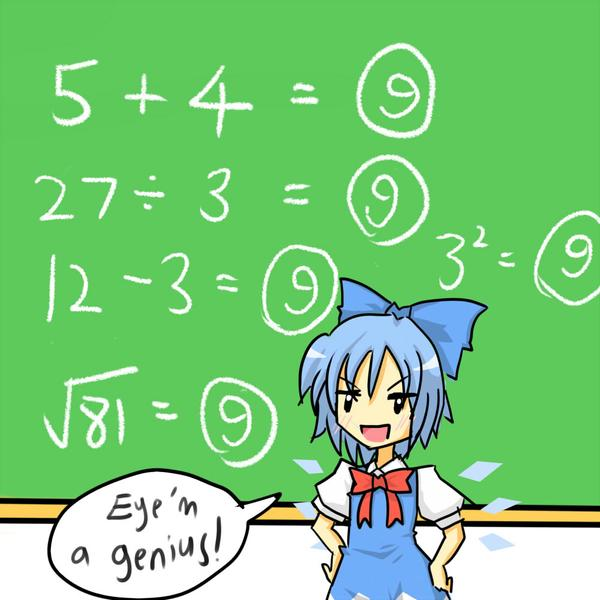
\includegraphics[width=0.8\textwidth]{images/genius_by_lunarisfuryaileron_d2qp8sd-fullview.jpg}}

\frontmatter
\maketitle
\tableofcontents

\mainmatter
\chapter{Spazi metrici e successioni di funzioni}

Si parla di spazi metrici quando si può definire su di essi una \textbf{metrica}, e si può quindi definire la coppia $(X,d)$.

\section{Distanze}

Sia un insieme di elementi $X \neq \emptyset$, definiamo come  \textbf{distanza} un'applicazione 
\begin{align}
d \, : \, X \times X {}&\rightarrow [0, + \infty) \\
(x,y) &\rightarrow d(x,y)
\end{align}
che rispetta le seguenti proprietà
\begin{enumerate}
	\item $d(x,y) \geq 0 \quad ; \quad d(x,y) = 0 \leftrightarrow x=y$
	\item $d(x,y)=d(y,x)$
	\item $d(x,y) \leq d(x,z) + d(z,y) \quad \forall x,y,z \in X$ \quad \text{[disuguaglianza triangolare]}
\end{enumerate}

\section{Intorni}

Sia $x_0 \in X$, si definisce un suo intorno di \textbf{raggio} $R$ come
\begin{align}
I(x_0,R) = \left\{x\in X \, : \, d(x,x_0)<R
\right\}
\end{align}

Gli intorni si dividono in due categorie:
\begin{enumerate}
	\item \textbf{Aperti}
	
	preso $A \subset X$, $A$ si dice aperto se 
	\begin{align}
	\forall x \in A \quad \exists \, R>0 \, : \, I(x,R)\subset A
	\end{align}
	
	\item \textbf{Chiusi}
	
	preso $C \subset X$, $C$ si dice chiuso se il suo complementare $\overline{C}= X \, \backslash \, C$ è aperto
\end{enumerate}
\newpage

\section{Esempi di metriche}

Vediamo degli esempi notevoli

\subsection{Metrica discreta}

\begin{align}
X \, : \, d(x,y) {}&= \left\{
\begin{array}{cc}
0  \qquad se \quad R<1\\
1  \qquad se \quad R>1
\end{array}
\right. \\
\nonumber \\
I(x,R) &= \left\{
\begin{array}{cc}
x  \qquad se \quad R<1\\
X  \qquad se \quad R>1
\end{array}
\right.
\end{align}

Si nota subito come le proprietà della distanza siano rispettate.

Notiamo che per come è definita la metrica, ogni sottoinsieme è discreto.

\subsection{Metrica Euclidea}

\begin{align}
X= \mathbb{R}^n \quad ; \quad x \in \mathbb{R}^n = (x_1, \dots , x_n) \\
d_n(x,y)= |x-y|_n = \sqrt{\sum_{i=1}^{n} (x_i - y_i)^2}
\end{align}

Verifichiamo come $d_n(x,y)$ sia una buona metrica.

Le prime due proprietà sono evidenti, la terza un po' meno.
\begin{align}
|x-y|_n \overset{?}{\leq}  |x-z|_n + |z-y|_n
\end{align}
definiamo
\begin{align}
{}&x-z = a \\
&z-y = b \\
&x-y = x-z + z-y = a + b
\end{align}
e riscriviamo
\begin{align}
|a+b|_n \overset{?}{\leq} |a|_n + |b|_n
\end{align}
Dimostrare questo è equivalente a dimostrare
\begin{align}
|a+b|_n^2 \overset{?}{\leq} (|a|_n + |b|_n)^2
\end{align}
Procediamo nel seguente modo:
\begin{align}
{}&|a+b|_n^2 \overset{?}{\leq} (|a|_n + |b|_n)^2 \nonumber \\
\downarrow \nonumber \\
&\sum_{i=1}^{n} (a_i + b_i)^2  \overset{?}{\leq} |a|^2_n + |b|^2_n + 2|a|_n|b|_n \nonumber \\
\downarrow \nonumber \\
&\sum_{i=1}^{n} a_i^2 + b_i^2 + 2a_ib_i \overset{?}{\leq} \sum_{i=1}^{n} a_i^2 + \sum_{i=1}^{n} b_i^2 + 2|a|_n|b|_n \nonumber \\
\downarrow \nonumber \\
&\sum_{i=1}^{n} a_ib_i \coloneqq \braket{a|b} \overset{?}{\leq} |a|_n|b|_n
\end{align}
Per verificare questo ci serve la \textbf{disuguaglianza di Cauchy-Shwartz}, che ricaviamo nel seguente modo:
\begin{align}
{}&\sum_{i=1}^{n} (a_i + t b_i)^2 \geq 0 \quad \forall t \in \mathbb{R} \nonumber \\
\downarrow \nonumber \\
& \sum_{i=1}^{n}(a_i^2 + b_i^2 + 2ta_ib_i ) \geq 0 \nonumber \\
\downarrow \nonumber \\
& |a|^2_n + |b|^2_n + 2t \sum_{i=1}^{n} a_ib_i \geq 0 \nonumber \\
\downarrow \nonumber \\
& |a|^2_n + |b|^2_n + 2t \braket{a|b} \geq 0 \quad \forall t\in \mathbb{R}
\end{align}
Quest'ultima disequazione rappresenta un luogo di punti contenuto in una parabola convessa che incrocia gli assi al massimo in un punto, quindi segue che $\Delta \leq 0$, ovvero

\begin{align}
{}&\Delta = 4 t^2 |\braket{a|b}|^2 - 4t^2|a|^2_n |b|^2_n \leq 0 \nonumber \\
\downarrow \nonumber \\
&|\braket{a|b}|^2 \leq |a|^2_n |b|^2_n \nonumber \\
\downarrow \nonumber \\
& |\braket{a|b}| \leq |a|_n |b|_n \quad \text{[disequazione di Cauchy-Shwartz]}
\end{align}

Siccome sappiamo che $a \leq |a| \, \forall a$ ne segue la nostra dimostrazione:

\begin{align}
\braket{a|b} \leq |\braket{a|b}| \leq |a|_n |b|_n \rightarrow 
\braket{a|b} \leq |a|_n |b|_n
\end{align}

in metrica euclidea gli intorni si dicono "circolari", dato che assumono forme del tipo:

\begin{align}
I(0,R)= \left\{ (x_1,x_2)\in \mathbb{R}^2 \, : \, \sqrt{x_1^2 + x_2^2}<R \right\}
\end{align}

che è l'equivalente di una circonferenza di raggio $R^2$.

\subsection{Metriche "equivalenti"}

Si parla di \textbf{metriche equivalenti} quando si ha che

\begin{align}
m,M>0 \; : \; m\delta(x,y) <d(x,y) < M \delta(x,y) \\
I_d(x,mR) \subset I_\delta(x,R) \subset I_d (x,MR)
\end{align}

In altri termini, in ogni intorno nella metrica $\delta$ posso avere un intorno della metrica $d$.

\smallskip

Alcuni esempi sono:

\begin{align}
{}&d_1(x,y) = \sqrt{\sum_{i=1}^{n} a_i (x_i - y_i)^2} \quad ; \quad a_i > 0 \, , \, a_i \in \mathbb{R} \\
&d_2(x,y) = \sum_{i=1}^{n} |x_i - y_i|_1 \\
&d_3(x,y) = \underset{i \in [1,n]}{Max} |x_i - y_i|_1
\end{align}

Tutti gli spazi su cui sono applicabili sono metrici, e gli intorni saranno del tipo:

\begin{align}
I_1(0,R) {}&= \left\{ (x_1,x_2) : \sqrt{a_1 x_1^2 + a_2 x_2^2} < R \right\} \quad \text{intorno circolare}\\
I_2(0,R) &= \left\{ (x_1,x_2) : |x_1| + |x_2|  < R
\right\} \quad \text{intorno romboidale} \\
I_3(0,R)&= \left\{ (x_1,x_2) : max(|x_1| , |x_2|)  < R
\right\}  \quad \text{intorno quadrato}
\end{align}

\section{Spazio delle funzioni continue}

\begin{align}
X= C^0([a,b])= \left\{ f \; : \; [a,b] \rightarrow \mathbb{R} \; \text{continue in } [a,b]
\right\}
\end{align}

Definiamo la \textbf{metrica uniforme} come
\begin{align}
d(f,g) = \underset{[a,b]}{sup}|f(x) - g(x)| = \underset{[a,b]}{Max}|f(x) - g(x)|= ||f-g||_\infty
\end{align}

Vediamo come rispetti le proprietà delle distanze:

Le prime due sono evidenti, dimostriamo solo la terza

GLI APPUNTI CHE MI HANNO GIRATO NON HANNO SENSO, VEDERE CON QUALCUNO

\bigskip

Possiamo quindi dire che $(C^0([a,b]), ||\cdot||_\infty)$ costituiscono uno spazio metrico.

\section{Spazi normati}

Si dice che uno spazio vettoriale $X$ è anche normato se vi è definibile
\begin{align}
||\cdot|| \; : \; X \rightarrow [0, +\infty)
\end{align}

con le seguenti proprietà:

\begin{enumerate}
	\item $||x|| \geq 0 \; , \; ||x||=0 \leftrightarrow x=0$
	\item $||\lambda x||= |\lambda| \, ||x|| \quad ; \quad \lambda \in \mathbb{R} \; , \; x \in X$
	\item $||x+y|| \leq ||x|| + ||y||$
\end{enumerate}

Possiamo fare le seguenti osservazioni:

\begin{enumerate}
	\item uno spazio normato $(X, ||\cdot||)$ è anche metrico con $d(x,y)= ||x-y||$
	\item $C^0([a,b])$ è spazio normato con $||x||= |x|_n = \sqrt{\sum x_i^2} \; : \; ||f||=||f||_\infty$
	\item $\mathbb{R}$ con la metrica discreta non è uno spazio normato, infatti 
	\begin{align}
	{}&||x||= d(x,0) \\
	&||\lambda x||= d(\lambda x, 0) = \left\{
	\begin{array}{cc}
	0 \quad x=0 \\
	1 \quad x\neq 0
	\end{array}
	\right.
	\end{align}
\end{enumerate}

\section{Tipologie di punti}

Sia uno spazio metrico $(X,d)$ con $D \subseteq X$, preso un $x \in D$, esso sarà, rispetto a $D$:

\begin{enumerate}
	\item \textbf{Interno}
	
		se  $\exists R >0 \; : \; I(x,R)\subset D$
		
		Osservazione: Se $D$ è aperto tutti i suoi punti sono interni, e viceversa.
	\item \textbf{Esterno}
	
		se  $\exists R >0 \; : \; I(x,R)\subset X \, \backslash \,D$
	\item \textbf{di Frontiera} ($x \in \partial D$)
	
		se $\forall R>0$ si ha $I(x,R)\cap D \neq \emptyset \neq I(x,R)\cap  X \, \backslash \,D$
		
		Si definisce \textbf{chiusura di D} l'insieme $\overline{D}= D \cup \partial D$
		
	\item \textbf{di Accumulazione}
	
		se $\forall R>0$ in $I(x,R)$ cade \underline{almeno} un punto di $D$ diverso da $x$.
		
		L'insieme dei punti di accumulazione $acc(D)$ prende il nume di \textbf{Derivato di D}.
\end{enumerate}

\textit{Osservazione}: $C$ chiuso $\leftrightarrow$ $\partial C \subseteq C$ $\leftrightarrow$ $acc(C) \subseteq C$ $\leftrightarrow$ $C= \overline{C}$

\newpage


\section{Successioni}

Sia (X,d) uno spazio metrico, si definisce come \textbf{successione di funzioni} come

\begin{align}
\left\{ x_k \right\}_{k\geq 1} \quad ; \quad x_k \in X
\end{align}

\subsection{Successioni convergenti}

Si dice che una successione $\left\{ x_k \right\}_{k\geq 1}\in X$ è convergente ad $x_0 \in X$ quando
\begin{align}
\underset{k\rightarrow 0}{\lim} \, d(x_k,x_0)=0 \quad \leftrightarrow \quad \underset{k\rightarrow 0}{\lim} \, x_k=x_0 \quad \leftrightarrow \quad x_k \overset{d}{\rightarrow} x_0
\end{align}

Vediamone alcuni \textbf{esempi:}

\begin{enumerate}
	\item in $\R$ avremo $\limit{k}{\infty} |x_k - x_0|_1=0 \implies \limit{k}{\infty}x_k=x_0$
	\item in $\R^n$ avremo $\limit{k}{\infty} |\vecx^{(k)} - \vecx^{0}|_n=0 \implies \vecx^{(k)}\overset{||\cdot||_\infty}{\longrightarrow}\vecx^{(k)}$
	\item $\vecx^{(k)}=(\half^k \spacecomma \fracn{\Exp{x^2}} \spacecomma \sin \left( \fracn{k} \right) ) \arrowlim{k}{\infty} (0,0,0) $
\end{enumerate}

cosa dubbiosa, cercare appunti altrui

\subsection{Successioni di Cauchy}

Dato uno spazio metrico $(X,d)$, una successione $\left\{ x_k \right\}_{k\geq 1}\in X$ si dice \textbf{di Cauchy} se
\begin{align}
\forall \epsilon > 0 \quad \exists n_\epsilon \; : \; d(x_{n+p},x_n)<\epsilon \quad \forall n>n_\epsilon \, , \, \forall p>0
\end{align}

Uno strumento utile è il seguente \textbf{teorema}:

\bigskip

\textit{se $\left\{ x_k \right\}_{k\geq 1}\in X$ converge ad $x^0$ allora è anche \textbf{di Cauchy}}.

\bigskip

La dimostrazione è semplice:
\begin{align}
d(x_{n+p}, x_n) \leq d(x_{n+p}, x^0) + d(x^0, x_p)
\end{align}

Siccome per ipotesi la successione è convergente avremo, $\forall n>n_\epsilon$
\begin{align}
{}&d(x_{n+p}, x^0) < \frac{\epsilon}{2} \\
&d(x^0, x_p) < \frac{\epsilon}{2}
\end{align}
e quindi
\begin{align}
d(x_{n+p}, x_n) \leq \frac{\epsilon}{2} + \frac{\epsilon}{2}=\epsilon
\end{align}
E il teorema è quindi dimostrato.

\bigskip

NOTA BENE: Non è detto il viceversa!

\newpage

\section{Spazi}

\subsection{Spazi compatti}

Si dice che uno spazio è \textbf{compatto} se $\forall \left\{ x_k \right\}_{k\geq 1}\in X$ è possibile ricavare una sottosuccessione convergente.

Un'altro modo per definire la compattezza è tramite il teorema di \textbf{Heine-Borel}, che afferma:

\bigskip

\textit{$A \subset \mathbb{R}$ è compatto \underline{se e solo se} $A$ è chiuso e compatto}

\subsection{Spazi completi}

Si dice che uno spazio $X$ è \textbf{completo} qualora ogni successione di Cauchy in esso converga ad un $x\in X$

\subsubsection{Spazi completi (Ex.)}

Tutti gli $(\mathbb{R}^n, ||\cdot||_n)$ sono spazi metrici completi. Diamo una dimostrazione semplice e poco approfondita:

\begin{align}
{}&\left\{ x_k \right\}_{k\geq 1} \in \mathbb{R}^n \; \text{succ. di cauchy} \nonumber \\
& \downarrow \nonumber \\
& \left\{ x_k \right\}_{k\geq 1} \; \text{è anche limitata} \nonumber \\
& \downarrow \nonumber \\
& \text{Possiamo applicare il th. di \textbf{Bolzano-Weierstrass}} \nonumber \\
& \downarrow \nonumber \\
& \exists \; \text{una sottosucc. conv. ad un generico } x^0 \nonumber \\
& \downarrow \nonumber \\
& \text{essendo di Cauchy anche } \left\{ x_k \right\} \rightarrow x^0 \nonumber
\end{align}

\subsubsection{Spazi \underline{non}  completi  (Ex.)}

\begin{enumerate}
	\item $(\mathbb{Q}, |\cdot|_1)$ non è completo, dato che 
	
	\begin{align}
	{}&x_n=\left(
	1+\frac{1}{n}
	\right)^n \in \mathbb{Q} \subset \mathbb{R} \\
	&\underset{n \rightarrow \infty}{\lim} \, x_n= e \notin \mathbb{Q}
	\end{align}
	
	\item X=(0,2)
	
	\begin{align}
	{}&x_n= \frac{1}{n} \in X \\
	& \underset{n \rightarrow \infty}{\lim} \, x_n = 0 \notin X
	\end{align}
\end{enumerate}

\subsubsection{$(C^0([a,b]), ||\cdot||_\infty)$  (Ex.)}

Dimostriamo come lo spazio delle funzioni continue sia completo in metrica $||\cdot||_\infty$

\bigskip


Sia $\left\{f_n(x)\right\} \in C^0([a,b])$ una successione di Cauchy, ovvero
\begin{align}
\forall \epsilon > 0 \; \exists n_\epsilon \; : \; ||f_{n+p} - f_n||< \epsilon \; \forall n>n_\epsilon \, , \, \forall p>0
\end{align}

Fissato $x\in [a,b]$ avremo
\begin{align}
|f_{n+p} - f_n| \leq || f_{n+p}(x) - f_n(x)||_\infty<\epsilon
\end{align}

Ne segue quindi che $\left\{f_n(x)\right\}$ è di Cauchy in $\mathbb{R}$, e siccome esso è completo questo vuol dire che abbiamo un candidato limite:
\begin{align}
\exists f(x)= \underset{n \rightarrow \infty}{\lim}f_n(x) \; \forall x\in [a,b]
\end{align}
Ora ci rimane da dimostrare che
\begin{enumerate}
	\item $f_n(x) \overset{||\cdot||_\infty}{\longrightarrow} f(x)$
	\item $f(x)  \in C^0([a,b])$
\end{enumerate}

Partiamo dal primo punto:

Abbiamo che
\begin{align}
|f_{n+p}(x) - f_n(x)|< \epsilon \quad \left\{
\begin{array}{ccc}
{}\forall n>n_\epsilon \\
\forall p>0 \\
\forall x \in [a,b]
\end{array}
\right.
\end{align}
Per costruzione sappiamo che
\begin{align}
\underset{p\rightarrow \infty}{\lim}f_{n+p}(x) = f(x)
\end{align}
Da cui
\begin{align}
{}&|f(x) - f_n(x)|< \epsilon \quad \left\{
\begin{array}{cc}
{}\forall n>n_\epsilon \\
\forall x \in [a,b]
\end{array}
\right. \\
&\downarrow \nonumber\\
&\underset{[a,b]}{sup}|f(x) - f_n(x)| \leq \epsilon \quad \forall n> n_\epsilon \\
&\downarrow \nonumber\\
& ||f(x) - f_n(x)||_\infty \leq \epsilon \quad \text{Q.E.D.}
\end{align}

Il secondo punto si dimostra nel seguente modo:

Possiamo scrivere, utilizzando la dis. triangolare
\begin{align}
|f(x) - f(x_0)| \leq |f(x) - f_n(x)| + |f_n(x_0) - f_n(x_0)| + |f_n(x_0) - f(x_0)|
\end{align}
Ma sappiamo che
\begin{align}
{}&|f(x) - f_n(x)|<\frac{\epsilon}{3} \quad \forall n>n_\epsilon \; \text{per convergenza uniforme}\\
&|f_n(x_0) - f_n(x_0)|<\frac{\epsilon}{3} \quad \forall x \, : \, |x-x_0|<\delta_\epsilon \; \text{per continuità} \\
&|f_n(x_0) - f(x_0)|<\frac{\epsilon}{3} \quad \forall n>n_\epsilon \; \text{per convergenza uniforme}
\end{align}
Da cui segue la dimostrazione con
\begin{align}
|f(x) - f(x_0)| \leq \epsilon
\end{align}

\subsection{Spazi di Banach}

Sono detti \textbf{di Banach} quegli spazi normati $(X,||\cdot||)$ che sono anche completi nella metrica indotta dalla norma.

\newpage

\section{Funzioni Continue}

Sia definita una funzione come un'applicazione del tipo
\begin{align}
f \, : \, (X,d_x) {}&\longrightarrow (Y,d_y)\\
x \in X &\longrightarrow y \in Y
\end{align}

Essa sarà continua in $x_0 \in X$ se 
\begin{align}
\forall \epsilon >0 \quad \exists \delta_\epsilon \, : \, d_x(x,x_0)<\delta_\epsilon \implies d_y(y,y_0)<\epsilon
\end{align}

\bigskip

Esempi di tali applicazioni posso essere:

\begin{enumerate}
	\item Funzione di una variabile
		\begin{align}
			f \, : \, \mathbb{R} \longrightarrow \mathbb{R}
		\end{align}
	\item Curva nel piano
		\begin{align}
			f \, : \, \mathbb{R} {}&\longrightarrow \mathbb{R}^2 \\
			t &\longrightarrow (x(t), y(t)) \nonumber
		\end{align}
	\item Curva nello spazio
		\begin{align}
			f \, : \, \mathbb{R} {}&\longrightarrow \mathbb{R}^3 \\
			t &\longrightarrow (x(t), y(t),z(t)) \nonumber
		\end{align}
	
	\item Superficie nello spazio
	
	\begin{align}
	f \, : \, \mathbb{R}^2 {}&\longrightarrow \mathbb{R}^3 \\
	(u,v) &\longrightarrow (x(u,v), y(u,v),z(u,v)) \nonumber
	\end{align}
	
	\item Funzionali (ex. l'integrale)
	
	\begin{align}
	T \, : \, C^0([a,b]) {}&\longrightarrow \mathbb{R} \\
	f &\longrightarrow T(f) \nonumber
	\end{align}
\end{enumerate}

\subsection{Lipschitzianità di una funzione}

Si dice che un'applicazione $T \, : \, X \longrightarrow X$ è Lipschitziana se 
\begin{align}
\exists L>0 \, : \, d(T_x, T_y) <L \, d(x,y) \quad \forall x,y \in X
\end{align}

(NOTA: $T_x= T(x)$ per eleganza)

\newpage

\subsection{Contrazioni}

Preso uno spazio $(X,d)$ le contrazioni sono una categoria di applicazioni continue e lipschitziane $T \, : \, X \longrightarrow X$ tali che
\begin{align}
d(T_x,T_y)<\alpha \, d(x,y) \quad \forall x,y \in X \, ; \, \alpha \in (0,1)
\end{align}

\subsubsection{Esempio di contrazione}
Dimostriamo come la seguente applicazione sia una contrazione
\begin{align}
T \, : \, C^0([0,1]) {}&\longrightarrow C^0([0,1]) \\
f & \longrightarrow T_f= 1 + \int_{0}^{1} dt \; t e^{-xt}f(t) \nonumber
\end{align}
\begin{align}
|T_{f(x)} - T_{g(x)}| {}&= |\int_{0}^{1} dt \; te^{-xt}[f(t) - g(t)]| \leq \nonumber \\
&\leq \int_{0}^{1} dt \; te^{-xt}|f(x) - g(x)|  \leq \nonumber \\
&\leq \int_{0}^{1} dt \; te^{-xt} \underset{[0,1]}{sup}|f(x) - g(x)|  \leq \nonumber \\
&\leq \int_{0}^{1} dt \; te^{-xt} ||f-g||_\infty=  ||f-g||_\infty \int_{0}^{1} dt \; te^{-xt}  \leq \nonumber \\
& \leq ||f-g||_\infty \int_{0}^{1} dt \; t = \frac{1}{2} ||f-g||_\infty
\end{align}

E quindi ne segue che $||T_f -T_g||_\infty \leq \frac{1}{2} ||f-g||_\infty$, che è una contrazione con $\alpha=\frac{1}{2}$

\subsubsection{Teorema di Banach-Cacciopoli (Principio di contrazione)}

Il principio di contrazione afferma che 
\bigskip

\textit{ Dati $(X,d)$ spazio metrico completo con $X\neq \emptyset$ e $T$ contrazione di $X$ in se stesso, avremo che $T$ \textbf{ammette un solo \underline{punto fisso}} $\overline{x} \, : \, T_{\overline{x}} = \overline{x}$}

\bigskip

Inziamo la dimostrazione prendendo $x_0 \in X$ e definendo una successione $\left\{ x_n\right\}_{n \geq 1} \in X$ per ricorrenza come
\begin{align}
x_1= T_{x_0}\;  , \; x_2 = T_{x_1} \;  , \; \dots \;  , \; x_{n+1} = T_{x_n}
\end{align}

Per prima cosa dimostriamo come essa sia di Cauchy:

Per costruzione e per definizione di contrazione avremo che
\begin{align}
d(x_1,x_2)= d(T_0,T_1)\leq \alpha \, d(x_0,x_1)
\end{align}

Da cui ricaviamo che 
\begin{align}
{}&d(x_2,x_3) \leq \alpha \, d(x_1,x_2) \leq \alpha^2 \, d(x_0,x_1) \nonumber \\
&\downarrow \nonumber \\
&d(x_n,x_{n+1}) \leq \alpha^2 \, d(x_{n-1},x_n) \leq \dots \leq \alpha^n \, d(x_0,x_1)
\end{align}

Da questo segue che, usando la disuguaglianza triangolare:
\begin{align}
d(x_{n+p}, x_n) {}&\leq d(x_{n+p}, x_{n+p-1}) + d(x_{n+p-1}, x_{n+p-2})  + \dots + \d(x_{n+1}, x_{n}) \leq \nonumber \\
& \leq (\alpha^{n+p-1} + \dots + \alpha^{n}) \, d(x_0,x_1)= \alpha^n \sum_{k=0}^{p-1}\alpha^k d(x_0,x_1) 
\end{align}
Ma la sommatoria è una ridotta della serie geometrica, di cui conosciamo la somma! Possiamo quindi scrivere
\begin{align}
d(x_{n+p}, x_n)  \leq  \alpha^n \frac{1-\alpha^{p-1}}{1-\alpha} \, d(x_0,x_1) \leq \frac{\alpha^n}{1-\alpha} \, d(x_0,x_1)
\end{align}

Ma notando come con le maggiorazioni sia sparita la dipendenza da p, e ricordando che $\alpha$ è infinitesimo, ricaviamo
\begin{align}
\underset{n\rightarrow \infty}{\lim}a^n=0 \implies d(x_{n+p}, x_n) < \epsilon \quad \forall n>n_\epsilon \, ; \, \forall p>0
\end{align}
E sono quindi verificate le ipotesi di Cauchy.

Ora che abbiamo questa informazione sappiamo anche che, nello spazio metrico completo $(X,d)$ avremo che 
\begin{align}
\exists \, \overline{x} \in X \, : \, \underset{n\rightarrow \infty}{\lim}x_n= \overline{x}
\end{align}

Dobbiamo ora dimostrare il suo essere un punto fisso:
\begin{align}
0 \leq d(T_{x_n}, T_{\overline{x}}) \leq \alpha \, d(x_n, \overline{x})\overset{n\rightarrow \infty}{\longrightarrow}0 \implies d(T_{x_n}, T_{\overline{x}}) =0
\end{align} 
ma per costruzione $T_{x_n}=x_{n+1}$, questo significa che
\begin{align}
 d(x_{n+1}, T_{\overline{x}})\overset{n\rightarrow \infty}{\longrightarrow}0 \implies \underset{n\rightarrow \infty}{\lim}x_{n+1}= \overline{x} = \underset{n\rightarrow \infty}{\lim}x_n
\end{align}
E per il teorema dell'unicità del limite segue che $T_{\overline{x}}=\overline{x}$

Rimane ora solo da dimostrarne l'unicità. Procediamo per assudro:

\begin{align}
\exists \hat{x},\overline{x} \in X \, , \, \hat{x}\neq \overline{x}  \, , \, T_{\hat{x}}=\hat{x} \, , \, T_{\overline{x}}=\overline{x} \\
0\leq d(\hat{x},\overline{x})= d(T_{\hat{x}},T_{\overline{x}}) \leq \alpha \, d(\hat{x},\overline{x}) < d(\hat{x},\overline{x})
\end{align}

Il che è impossibile, perché ci troviamo ad avere una distanza strettamente minore di se stessa, essendo $\alpha <1$. Il teorema è così dimostrato.

\newpage

\section{Successioni di funzioni}

Si parla di successioni di funzioni quando si ha
\begin{align}
\left\{f_n \right\}_{n\geq 1} \quad ; \quad f_n \, : \, I \subseteq \mathbb{R} \longrightarrow \mathbb{R}
\end{align}

\subsection{Criteri di convergenza}

\subsubsection{Convergenza Puntuale}

Si dice che $\left\{f_n \right\}_{n\geq 1}$ converge \textbf{puntualmente} in $I$ se
\begin{align}
\forall x\in I \quad  \exists f(x) \, : \, \underset{n\rightarrow \infty}{\lim} f_n(x)= f(x)
\end{align}

In simboli si scrive $f_n(x) \longrightarrow f(x)$

\subsubsection{Convergenza Uniforme}

Si dice che $\left\{f_n \right\}_{n\geq 1}$ converge \textbf{uniformemente} a $f(x) \, : \, I \subseteq \mathbb{R} \longrightarrow \mathbb{R}$ in $I$ se
\begin{align}
\underset{n\rightarrow \infty}{\lim} \underset{x\in I}{sup}| f_n(x) - f(x)|=0
\end{align}

Si può anche scrivere $\underset{n\rightarrow \infty}{\lim} \underset{x\in I}{sup}| f_n(x) - f(x)| = ||f_n(x) - f(x)||_\infty$ ma si perde l'informazione dell'intervallo.

\bigskip

In simboli si scrive $f_n(x) \rightrightarrows f(x)$

\bigskip

\textbf{Osservazione:} La convergenza uniforma implica quella puntuale, infatti siccome
\begin{align}
x \in X \quad | f_n(x) - f(x)| \leq\underset{x\in I}{sup}| f_n(x) - f(x)|
\end{align}

Se c'è convergenza uniforme allora $\leq\underset{x\in I}{sup}| f_n(x) - f(x)|$ è infinitesimo, allora
\begin{align}
0 \leq| f_n(x) - f(x)| \leq \underset{x\in I}{sup}| f_n(x) - f(x)|<\epsilon 
\end{align}

Da cui seguen la conv. puntuale.

\subsubsection{Esempi}

\begin{enumerate}
	\item $f_n(x)=x^n \spacer x \in [0,1]$
	\begin{enumerate}
		\item \underline{convergenza puntuale}
		\begin{align}
		f_n(x) =  \triple{0 \quad {}&x=0 }{x^n \quad &x\in (0,1)}{1 \quad &x=1} \arrowlim{n}{\infty} f(x)=\double{0 \quad {}& x\in [0,1)}{1 \quad &x=1}
		\end{align}
		\item \underline{convergenza uniforme}
		\begin{align}
		\{f_n(x)\}\in C^0([0,1])
		\end{align}
		Se $f_n(x)\underset{[0,1]}{\rightrightarrows} f(x)$ allora $\{f_n(x)\}$ è di Cauchy in $C^0([0,1])$
		
		Ma allora, essendo  $C^0([0,1])$ uno spazio metrico completo anche $f(x)$ dovrebbe appartenervi, ma ciò non è perché è discontinua. Quindi non c'è convergenza uniforme in $[0,1]$.
	\end{enumerate}
	
	\newpage
	
	\item $f_n(x)= \sqrt{x^2 + \frac{1}{n^2}}$
		\begin{enumerate}
		\item \underline{convergenza puntuale}
		\begin{align}
		f_n(x) \arrowlim{n}{\infty} \sqrt{x^2}=|x| =f(x)
		\end{align}
		\item \underline{convergenza uniforme}
		\begin{align}
		0\leq \left( \sqrt{x^2 + \frac{1}{n^2}} - \sqrt{x^2}=  \right) {}&= \left( \sqrt{x^2 + \frac{1}{n^2}} - \sqrt{x^2}  \right) \frac{ \sqrt{x^2 + \frac{1}{n^2}} + \sqrt{x^2}  }{\sqrt{x^2 + \frac{1}{n^2}} + \sqrt{x^2}} = \continue 
		&= \frac{x^2 + \frac{1}{n^2} - x^2}{\sqrt{x^2 + \frac{1}{n^2}} + \sqrt{x^2}} = \continue
		&= \fracn{\sqrt{x^2 + \frac{1}{n^2}} + \sqrt{x^2}}\fracn{n^2} \leq \continue
		&\leq \fracn{\fracn{n}}\fracn{n^2} = \fracn{n}\arrowlim{n}{\infty}0
		\end{align}
		
		Non dipendendo da $x$ il sup e annullandosi abbiamo convergenza uniforme su tutto $\R$.
		
	\end{enumerate}

	\item $f_n(x) = \triple{nx \quad {}&x\in[0,n^{-1}]}{2-nx \quad &x\in (n^{-1}, 2\cdot n^{-1})}{0 \quad &x\in [2 \cdot n^{-1},1]}$
	\begin{enumerate}
	\item \underline{convergenza puntuale}
	\begin{align}
	{}&f_n(0) = 0 \arrowlim{n}{\infty}0\\
	& \text{per }x>0 \text{ avremo che per n molto grandi } x\in (\frac{2}{n} \spacecomma 1] \nextpassage
	&f_n(x)=0 \arrowlim{n}{\infty}0 \quad \forall n>\frac{2}{\lambda}
	\end{align}
	
	Abbiamo quindi convergenza puntuale a $f(x) \equiv 0$
	\item \underline{convergenza uniforme}
	\begin{align}
	\Sup{I} |f_n(x)-0|= \underset{I}{max}f_n(x)=f_n\left(\fracn{n}\right)=1 \notends 0
	\end{align}
		E quindi non si ha convergenza uniforme.
	
	\end{enumerate}
	
	\item $f_n(x)= (1-x)x^n \quad x \in [0,1]$
	\begin{enumerate}
		\item \underline{convergenza puntuale}
		\begin{align}
		{}&f_n(0) = 0  \arrowlim{n}{\infty}0 \\
		&f_n(x) \arrowlim{n}{\infty}0 \quad x\in (0,1)\\
		&f_n(1)= 0 \arrowlim{n}{\infty}0 
		\end{align}
		
		Abbiamo quindi convergenza puntuale a $f(x)\equiv 0$
		
		\item \underline{convergenza uniforme}
		\begin{align}
		||(1-x)x^n  - 0||_\infty = \underset{I}{max} (1-x)x^n = \underset{I}{max}\, g(x) \geq 0 
		\end{align}
		
		Per trovare questo massimo procediamo nel seguente modo
		\begin{align}
		{}&g(x)= (1-x)x^n 	\implies g'(x)= -x^n + (1-x)nx^{n-1} \nextpassage
		& x^{n-1} (n-xn-x) = x^{n+1}[n(1+n)x]=0 \nextpassage &\double{x_0=0}{x_1=\frac{n}{1+n}<1} \implies \double{g(x_0)=0}{g(x_1)= \frac{1}{1+n} (\frac{n}{1+n})^n >0}
		\end{align}
				
		Il punto di max è chiaramente $x_1$, quindi ci troviamo a studiare		
		\begin{align}
		||(1-x)x^n  - 0||_\infty {}&= \underset{I}{max}\, g(x) = g(x_1)= \left(1-\frac{n}{n+1}\right) \left(\frac{n}{n+1}\right)^n= \continue
		&= \frac{1}{n+1}\left(\frac{1}{\fracn{n} +1}\right)^n \arrowlim{n}{\infty} 0 \cdot \fracn{e}=0
		\end{align}
		
		Essendo il risultato indipendente da $x$ abbiamo convergenza uniforme su tutto $\R$.		
	\end{enumerate}
	
	\item $f_n(x)=\frac{nx}{1+ (nx)^2} \spacer I=[-1,+1]$
	\begin{enumerate}
		\item \underline{convergenza puntuale}
		\begin{align}
		f_n(x) =  \double{0 \quad {}&x=0}{f_n(x) \quad &x\neq 0} \arrowlim{n}{\infty} 0 \implies f(x) \equiv 0
		\end{align}
		\item \underline{convergenza uniforme}
		\begin{align}
		||f_n(x) - 0||_\infty = \underset{I}{max} \absval{\frac{nx}{1+ (nx)^2}}
		\end{align}
		
		Poniamo $t= nx$ e studiamo $g(t)= \frac{t}{1+ t^2}$
		\begin{align}
		g'(t){}&= \frac{1}{1 + t^2} - 2\frac{t^2}{(1+t^2)^2} = \continue
		&= \frac{1 + t^2 -2t^2}{(1+t^2)^2}=\frac{1 -t^2}{(1+t^2)^2}=0 \implies \double{t_1 = -1}{t_2 = +1}
		\end{align}
		
		Da cui avremo che il punto di massimo si ha per $x_M = \fracn{n}$, e quindi
		
		\begin{align}
		||f_n(x) - 0||_\infty = \underset{I}{max} \absval{\frac{nx}{1+ (nx)^2}}= \frac{1}{1+1}=\half \notends 0
		\end{align}
		E non si ha quindi convergenza uniforme.	
	\end{enumerate}
	
\end{enumerate}

\subsection{Teoremi sulle successioni}

\subsubsection{Primo Teorema}

\textit{
Date $\left\{f_n \right\}_{n\geq 1}$ con $f_n(x)\in C^0(I)$ $I\subseteq \mathbb{R}$, avremo che}
\begin{align}
f_n(x) \rightrightarrows f(x) \implies f(x)\in C^0(I)
\end{align}

\textbf{Osservazione:} $I=[a,b]$ segue dalla completezza di $C^0([a,b])$ 

\bigskip

Dimostriamo il teorema:
\begin{align}
f_n(x) \rightrightarrows f(x) \implies \forall \epsilon >0 \quad \exists n>n_\epsilon \, : \, \underset{x\in I}{sup}| f_n(x) - f(x)|<\epsilon 
\end{align}
Per la disuguaglianza triangolare avremo che
\begin{align}
|f(x)-f(x_0)| \leq |f(x) - f_{n_\epsilon + 1}(x)|+|f_{n_\epsilon + 1}(x)- f_{n_\epsilon + 1}(x_0)|+|f_{n_\epsilon + 1}(x_0) - f(x_0)|
\end{align}
Ma sappiamo che
\begin{align}
{}& |f(x) - f_{n_\epsilon + 1}(x)|\leq||f_{n_\epsilon + 1}(x) - f(x)||_\infty <\epsilon \\
& |f_{n_\epsilon + 1}(x)- f_{n_\epsilon + 1}(x_0)|<\epsilon \quad \text{per continuità di }f_{n_\epsilon + 1} \\
& |f_{n_\epsilon + 1}(x_0) - f(x_0)| \leq||f_{n_\epsilon + 1}(x_0) - f(x_0)||_\infty <\epsilon 
\end{align}
E quindi segue che
\begin{align}
\forall \epsilon>0  \quad \exists \delta_\epsilon \, : \, |f(x)-f(x_0)| < 3\epsilon \quad \forall x \, : \, |x-x_0|<\delta_\epsilon
\end{align}
e il teorema è dunque dimostrato.

\subsubsection{Secondo Teorema (Scambio Limite e Integrale)}
\textit{
Date $\left\{f_n \right\}_{n\geq 1}$ con $f_n(x)\in C^0([a,b])$ $[a,b]\subseteq \mathbb{R}$, avremo che}

\begin{align}
f_n(x)\underset{[a,b]}{\rightrightarrows} f(x) \implies \int_{a}^{b} dt \, \underset{n\rightarrow \infty}{\lim}f_n(t)= \underset{n\rightarrow \infty}{\lim} \int_{a}^{b} dt \, f_n(t) 
\end{align}
\textit{e quindi anche}
\begin{align}
\int_{a}^{b} dt \, f(t)= \underset{n\rightarrow \infty}{\lim} \int_{a}^{b} dt \, f_n(t)
\end{align}

La dimostrazione si svolge nel seguente modo
\begin{align}
\left|\int_{a}^{b} dt \, f_n(t) - \int_{a}^{b} dt \, f(t)\right| {}&= \left|\int_{a}^{b} dt \, [f_n(t) -  f(t)]\right| \leq \nonumber \\
&\leq \int_{a}^{b} dt \, |f_n(t) -  f(t)| \leq \nonumber \\
&\leq \int_{a}^{b} dt \, \underset{[a,b]}{max}|f_n(x) -  f(x)| = \nonumber \\
&= \int_{a}^{b} dt ||f_n(x) -  f(x)||_\infty = \nonumber \\
&= ||f_n(x) -  f(x)||_\infty \int_{a}^{b} dt = \nonumber \\
&=||f_n(x) -  f(x)||_\infty (b-a)
\end{align} 

Ma se $f_n(x) \rightrightarrows f(x)$ segue che $||f_n(x) -  f(x)||_\infty \overset{n\rightarrow \infty}{\longrightarrow} 0$

Da cui, ricordando che il modulo è una quantità non negativa, otteniamo il risultato desiderato:
\begin{align}
0 \leq \left|\int_{a}^{b} dt \, f_n(x) - \int_{a}^{b} dt \, f(x)\right| \leq 0
\end{align}

\subsubsection{Terzo Teorema (Scambio Derivata e Limite)}

Siccome abbiamo visto come sotto determinate condizioni è possibile scambiare anche derivata e limite. 

Come per l'integrale, la risposta in generale è: \textbf{No}, comke vediamo negli esempi che seguono.

\begin{enumerate}
	\item $f_n(x)= \sqrt{x^2 + \frac{1}{n}} \quad; \quad x\in I\subseteq \mathbb{R}$
		
		Infatti
		\begin{align}
		f_n'(x)= \frac{x}{\sqrt{x^2 + \frac{1}{n}}} \implies f_n'(0) = 0 
		\end{align}
		Ma
		\begin{align}
		\underset{n\rightarrow \infty}{\lim} f_n(x)= |x|
		\end{align}
		Che non è derivabile in 0.
	
	\item $f_n(x) = \frac{\sin(nx)}{n}\in \mathbb{R} \; \text{oppure} \; [a,b]$ 
		\begin{align}
		{}&f_n'(x)=\cos(nx)\\
		&\underset{n\rightarrow \infty}{\lim} f_n(x)= \left\{
		\begin{array}{cc}
			0 \quad nx=0  \quad \quad \quad \quad \;\; \\
			0 \quad nx \, : \, sin(nx) \neq 0
		\end{array}
		\right. \implies f(x) \equiv 0 = f'(x)
		\end{align}
	
	Ma $\nexists \underset{n\rightarrow \infty}{\lim} cos(nx)$, e quindi non si possono scambiare.
\end{enumerate}	 

Enunciamo quindi il \textbf{Teorema di Scambio tra Derivata e Limite:}

\bigskip

\textit{Sia $\left\{f_n\right\}$ con $f_n(x) \in C^1([a,b])$ se valgono le seguenti ipotesi: }
\begin{enumerate}
	\item $\exists x_0 \in [a,b] \, : \, f_n(x_0) \overset{n\rightarrow \infty}{\longrightarrow} l\in \mathbb{R}$
	
	\item $\left\{f'_n\right\} \, : \, f'_n(x) \rightrightarrows g(x)$ 
\end{enumerate}

\smallskip

\textit{Allora segue che:}
\begin{enumerate}
	\item $f_n \rightrightarrows  f(x)$
	\item $f(x)\in C^1([a,b]) \, ; \, f'(x) =g(x) \leftrightarrow f'(x)= \frac{d}{dx} \underset{n\rightarrow \infty}{\lim}f_n(x)=  \underset{n\rightarrow \infty}{\lim} \frac{d}{dx}f_n(x) $
\end{enumerate}		

Per la dimostrazione si parte dal th. fondamentale del calcolo, che ci dice:
\begin{align}
	f_n(x)=f_n(x_0) + \int_{x_0}^{x} dt \, f_n'(x)
\end{align}
Da cui otteniamo, passando a limite
\begin{align}
	\underset{n\rightarrow \infty}{\lim} f_n(x)=l +  \underset{n\rightarrow \infty}{\lim}\int_{x_0}^{x} dt \, f_n'(t)
\end{align}
ma siccome le ipotesi sono le stesse del th. di scambio fra limite e integrale scriviamo
\begin{align}
	\underset{n\rightarrow \infty}{\lim} f_n(x)=l +  \int_{x_0}^{x} dt \, g(t)
\end{align}
Ma questo implica che
\begin{align}
	\exists f(x)= l +  \int_{x_0}^{x} dt \, g(t) \quad \forall x\in[a,b] \,: \, f_n(x) \longrightarrow f(x)
\end{align}
Questo ci porta ad avere
\begin{align}
	|f_n(x)- f(x)| {}&= |f_n(x_0) - l + \int_{x_0}^{x} dt \, [f'_n(t) - g(t)]| \leq \nonumber \\ 
	&\leq |f_n(x_0) - l| + |\int_{x_0}^{x} dt \, [f'_n(t) - g(t)]|\leq \nonumber \\ 
	&\leq |f_n(x_0) - l| + ||f'_n(t) - g(t)||_\infty|x-x_0| \leq \nonumber \\ 
	&\leq |f_n(x_0) - l| + ||f'_n(t) - g(t)||_\infty |b-a|
\end{align}

Ma sappiamo che
\begin{align}
	{}& |f_n(x_0) - l|<\epsilon \quad \text{per continuità delle } f_n(x)\\
	& ||f'_n(t) - g(t)||_\infty <\epsilon \quad \text{per la seconda ipotesi del teorema}
\end{align}
Questo implica, essendo entrambi \textbf{strettamente minori}, che anche
\begin{align}
	||f_n(x_0) - l||_\infty<\epsilon \quad \forall x\in[a,b]\, , \, \forall n>n_\epsilon
\end{align}

Questo dimostra la prima tesi, mentre la seconda di nuovo dal th. fondamentale del calcolo, in quanto
\begin{align}
	f(x)=f(x_0) + \int_{x_0}^{x} dt \, f'(x)
\end{align}
ma
\begin{align}
	f(x)= \underset{n\rightarrow \infty}{\lim} f_n(x)= l +  \int_{x_0}^{x} dt \, \underset{n\rightarrow \infty}{\lim} f_n'(t)
\end{align}
e dato che per conitnuità $f(x_0)=l$, sottraendo membro a membro otteniamo infine che
\begin{align}
	f'(x) = \underset{n\rightarrow \infty}{\lim} f_n'(t)
\end{align}

\newpage

\subsection{Completezza di $C^1([a,b])$}

Abbiamo visto come $C^0$ sia completo con la norma $d_0(f,g)=||f-q||_\infty$

Ci chiediamo ora: con quale metrica sarà completo $C^1$? Non con $d_0(f,g)$, visto che
\begin{align}
	f_n(x)= \sqrt{x^2 + \frac{1}{n}} \rightrightarrows |x| \quad x\in[-1,+1]
\end{align} 
Che è sì di cauchy, ma non converge ad una funzione di classe $C^1$.

Introduciamo quindi la seguente metrica
\begin{align}
	d_1(f,g) {}&= \underset{[a,b]}{sup}|f(x)-g(x)|+\underset{[a,b]}{sup}|f'(x)-g'(x)| = \\ 
	&=||f(x)-g(x)||_\infty + ||f'(x)-g'(x)||_\infty
\end{align}

Con questa metrica avremo che se $\left\{f_n(x)\right\}$ è di Cauchy in $(C^1([a,b]),d_1)$ allora
\begin{align}
	{}&||f(x)-g(x)||_\infty < \epsilon \\
	&||f'(x)-g'(x)||_\infty < \epsilon
\end{align}

Questo vuol dire che entrambe sono di Cauchy in $(C^0([a,b]),d_0)$, e che sono anche verificate le ipotesi del teorema di scambio fra derivata e limite, e troviamo quindi che
\begin{align}
	\left\{
	\begin{array}{cc}
		f(x)\in C^1([a,b]) \\
		f_n'\rightrightarrows f'(x)
	\end{array}
	\right. \implies f_n \overset{d_1}{\longrightarrow} f \in C^1([a,b])
\end{align}
E quindi $(C^1([a,b]),d_1)$ è completo.

Un altro esempio di metrica in cui $C^1$ è completo si ha, preso ad esempio l'intervallo $[0,1]$ con 
\begin{align}
	\tilde{d}(f,g) {}&= |f(x) - g(x)| + \Sup{[0,1]}|f'(x) - g'(x)| = \continue
	&= |f(x) - g(x)| + ||f'(x) - g'(x)||_\infty
\end{align}

Data $\{f_n(x)\}\in C^1([0,1])$ se è di Cauchy allora $f_n(x) \overset{\tilde{d}}{\longrightarrow} f(x)$

Deve essere inoltre che
\begin{align}
	\forall \epsilon> 0 \quad \exists n_\epsilon \taleche |f_{n+p} - f_n| + ||f_{n+p}' - f_n'||_\infty<\epsilon \quad  \begin{array}{cc}
		\forall n>n_\epsilon \\
		\forall p>0
	\end{array}
\end{align}

Ma questo implica che
\begin{align}
	{}&|f_{n+p}(0) - f_n(0)| < \epsilon \implies \{f_n(0)\} \text{ di Cauchy in } \R \text{ completo} \\
	& ||f_{n+p}' - f_n'||_\infty<\epsilon \implies \{f_n'\} \text{ di Cauchy in } (C^0([a,b]), ||\cdot||_\infty) 
\end{align}

La seconda implica anche che $f'(x) \rightrightarrows g(x) \in (C^0([a,b])$, e abbiamo quindi tutte le ipotesi del th. di scambio tra limite e derivata!

Ci troviamo quindi a lavorare con una metrica che fa sì che
\begin{align}
	{}&f_n \overset{\tilde{d}}{\longrightarrow} f\\
	& f'_n \overset{\tilde{d}}{\rightrightarrows} f'
\end{align}

E abbiamo quindi la completezza di $C^1$ con la metrica $\tilde{d}$.

\bigskip

Chiudiamo il discorso delle successioni di funzioni con un \textbf{esempio}:
\begin{align}
	f_n(x)= \frac{x[(nx)^2 -2]}{(nx)^2 +1}
\end{align}

\begin{enumerate}
	\item \underline{convergenza puntuale:}
	\begin{align}
		\limit{n}{\infty}\frac{x[(nx)^2 -2]}{(nx)^2 +1}= \double{0 \quad {}&x=0}{x \quad &x=0}
	\end{align}
	\item \underline{convergenza uniforme:}
	\begin{align}
		\Sup{\R}\absval{\frac{x[(nx)^2 -2]}{(nx)^2 +1} -x} = \Sup{\R}\absval{\frac{x}{(nx)^2 +1}}
	\end{align}
\end{enumerate}

In modo analogo ad altri esercizi studiamo la derivata della $f_n(x)$ e troviamo un punto di massimo in $x= \frac{1}{n}$ da cui
\begin{align}
	\Sup{\R}\absval{\frac{x}{(nx)^2 +1}} = \frac{\frac{1}{n}}{(n\frac{1}{n})^2 +1} = \fracn{2n} \arrowlim{n}{\infty}0
\end{align}

E abbiamo quindi convergenza uniforme.


\chapter{Curve ed integrali curvilinei}

\section{Curve}

Si definiscono \textbf{Curve nello spazio} quelle applicazioni
\begin{align}
	\underline{r}(t) \, : \, [a,b] {}&\longrightarrow \mathbb{R}^3 \\
	t &\longrightarrow (x(t),y(t),z(t))
\end{align}
con 
\begin{align}
&\underline{r}(t)=(x(t),y(t),z(t)) \in C^0([a,b]) \; ; \; |r(t)|=\sqrt{x^2(t) + y^2(t) + z^2(t)} \\
&\gamma = \left\{ x(t),y(t),z(t), t\in [a,b]
\right\} \subset \mathbb{R}^3 \quad \text{sostegno della curva}
\end{align}
Se $z(t)=0$ si parla di \textbf{Curve nel piano}.

\subsection{Curve regolari}

Si dice che una curva è \textbf{regolare} se
\begin{enumerate}
	\item $\underline{r}(t)=(x(t),y(t),z(t)) \in C^1([a,b])$
	\item $\underline{r}'(t)= (x'(t),y'(t),z'(t)) \neq (0,0,0) \leftrightarrow |r'(t)|>0$
\end{enumerate}

Mentre si parla di curve \textbf{regolari a tratti} quando non c'è regolarità complessiva ma si può scomporre in sottocurve regolari.

la comodità di lavorare con le curve regolari sta, fra le altre cose, nel poter definire il \textbf{Versore tangente} alla curva:
\begin{align}
\underline{T}= \frac{(x'(t),y'(t),z'(t))}{|r'(t)|}
\end{align}
e la \textbf{Retta tangente} alla curva in un punto $(x_0,y_0,z_0)\in \gamma$:
\begin{align}
\left\{
\begin{array}{ccc}
x(t)= x_0 + x'(t_0)(t-t_0) \\
y(t)= y_0 + y'(t_0)(t-t_0) \\
z(t)= z_0 + z'(t_0)(t-t_0)
\end{array}
\right.
\end{align}

Dal punto di vista cinematico, le quantità riguardanti le curve regolari possono essere viste come:

\begin{enumerate}
	\item $\underline{r}'(t)$ è il vettore velocità
	\item $|r'(t)|$ è la velocità tangente
	\item $\underline{r}''(t)$ è il vettore accelerazione (solo se $\underline{r}(t)\in C^2$)
\end{enumerate}

\subsubsection{Esempi di curve regolari a tratti}

\begin{enumerate}
	\item $\underline{r}(t)=(t,|t|, t^3) \quad ; \quad t\in(-1,3)$
	
	Questa curva non è regolare, essendo $|t|\notin C^1((-1,3))$, ma può essere spezzata in due curve con la stessa rappresentazione negli intervalli $(-1,0)$ e $(0,3)$
	che sono invece regolari.
	
	\item $\underline{r}(t)=(t^3,t^2) \quad ; \quad t\in(-1,+1)$ 
	
	Questa non è regolar in 0, dove si annullano le derivate, ma lo è a tratti nello stesso modo della precedente 
\end{enumerate}


\subsection{Curve semplici}
	
	Si dice che una curva è \textbf{semplice} se $\underline{r}(t)$ è iniettiva in $(a,b)$ ($\underline{r}(t_1) \neq \underline{r}(t_2) \leftrightarrow t_1 \neq t_2$) o, in parole povere, non si "attorciglia". Gli estremi sono esclusi, altrimenti non si potrebbero avere curve semplici chiuse.
	
	Un esempio sono tutti i grafici di funzione su $\mathbb{R}$.
	
\subsection{Curve equivalenti}

Dati
\begin{align}
&\underline{r}(t) \, : \, [a,b] \longrightarrow \mathbb{R}^3 \\
&\tilde{\underline{r}}(\tau) \, : \, [\alpha,\beta] \longrightarrow \mathbb{R}^3
\end{align}

Due curve $(\underline{r}(t),\gamma)$ e $ (\tilde{\underline{r}}(\tau), \tilde{\gamma})$ si dicono \textbf{equivalenti} se
\begin{align}
&\exists \phi \, : \, [\alpha,\beta] \longrightarrow [a,b] \quad ; \quad \phi \in C^1([\alpha,\beta])\\
&\exists \phi^{-1} \, : \, [a,b] \longrightarrow [\alpha,\beta]  \quad ; \quad  \phi^{-1} \in C^1([a,b])
\end{align}

Ovvero abbiamo un \textbf{diffeomorfismo} tale che $\underline{r}(\phi(t))=\tilde{\underline{r}}(\tau)$

Se $\phi(\tau)>0$ gli estremi delle curve saranno uguali, altrimenti saranno invertiti.

\subsection{Lunghezza di una curva}

Consideriamo la curva $\gamma$ di sostegno $[a,b]$ in figura
\begin{figure}[!htb]
	\center{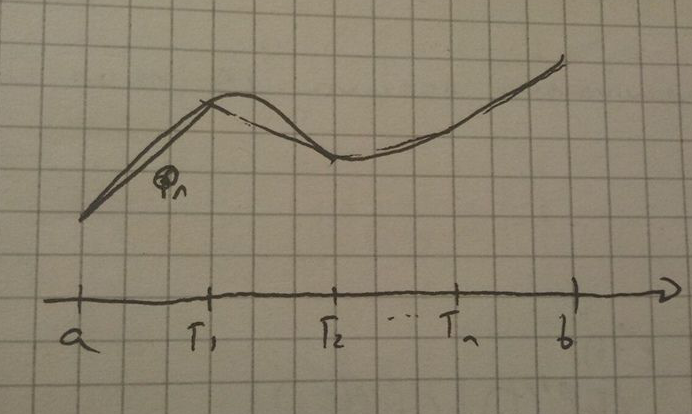
\includegraphics[width=0.5\textwidth]
		{images/curva.png}
		\caption{\label{fig:my-label}}}
\end{figure}

Una volta partizionato il sostegno in n infinitesime parti ed  individuata una spezzata poligonale $p(t)$ inscritta in $\gamma$ possiamo definire la lunghezza di $\gamma$ come
\begin{align}
lung(\gamma) = \underset{\gamma}{sup}|lung(p)|
\end{align}

Ma c'è un problema: chi ci dice che questa quantità è finita? Nessuno.

Diciamo allora che una curva è \textbf{rettificabile} se la sua lunghezza è finita.

Questa definizione è però troppo vaga per essere di utilità operativa, enunciamo quindi senza dimostrazione ("Sono pagine di conti che a noi non interessano" [cit. Lanzara]) il seguente \textbf{Teorema}:

\bigskip

\textit{Se una curva è regolare o regolare a tratti allora è rettificabile, e si avrà}
\begin{align}
lung(\gamma)=\int_{a}^{b} dt \, |r'(t)|= \int_{a}^{b} dt \, \sqrt{(x'(t))^2 + (y'(t))^2 + (z'(t))^2}
\end{align}

\textbf{Nota:} Per le curve regolari a tratti avremo $lung(\gamma)=\sum_{i=1}^{n}lung(\gamma_n)$

\bigskip

\subsubsection{Esempio: Elica Cilindrica}

$\underline{r}(t)=(R\cos(t), R\sin(t), ct) \quad; \quad t\in[0,2\pi] \, , R>0 \, c>0$

Notiamo come la curva sia regolare, essendo tutte le componenti di classe quantomeno $C^1([0,2\pi])$ ed essendo $|r'(t)|\neq (0,0,0) \; t\in(0,2\pi)$ essendo $c>0$

Avremo allora 
\bigskip

$lung(\gamma)=\int_{0}^{2\pi} dt \, \sqrt{R^2 + c^2}= 2\pi\sqrt{R^2 + c^2}$

\newpage

\subsubsection{Forma cartesiana}

Sia $y=f(x)\in C^1([a,b]) \; ; \; x\in[a,b]$, possiamo scrivere
\begin{align}
\underline{r}(t)=\left\{
\begin{array}{cc}
x=t \quad \;\,\\
y=f(t)
\end{array}
\right. \implies
lung(l)= \int_{a}^{b} dt \, \sqrt{1+ (f'(t))^2}
\end{align}

Che può però risultare scomoda, come vediamo nel seguente esempio:
\begin{align}
{}&y=f(x)=x^2 \; x\in [0,1] \implies f'(x)=2x \; f(x)\in C^1([0,1]) \\ 
&lung(l)= \int_{0}^{1} dx \, \sqrt{1+4x^2} \rightarrow \left\{
\begin{array}{cc}
t=2x \\
dt=2dx
\end{array}
\right. \rightarrow \frac{1}{2}\int_{0}^{2} dt \, \sqrt{1+t^2}
\end{align}
Facendo la sostituzione
\begin{align}
{}&t= \sinh(y)\\
&dt= \cosh(y)dy \\
&t \in [0,2] \rightarrow y \in [0,\overline{y}]
\end{align}
Avremo
\begin{align}
lung(l) {}&= \frac{1}{2} \int_{0}^{\overline{y}} dy \, \cosh(y)\sqrt{1 + \sinh^2(y)}= \nonumber \\
&=\frac{1}{2} \int_{0}^{\overline{y}} dy \, \cosh(y)\sqrt{\cosh^2(y)}= \nonumber \\
&= \frac{1}{2} \int_{0}^{\overline{y}} dy \, \cosh^2(y)= \nonumber \\
&= \frac{1}{4} \int_{0}^{\overline{y}} dy \, [1+\cosh(2y)]= \nonumber \\
&= \frac{1}{4} \left(\overline{y} + \frac{1}{2}\sinh(2\overline{y})\right)
\end{align}

\subsubsection{Lunghezze di curve equivalenti}

Supponiamo di avere due curve equivalenti $(\underline{r},\gamma)$ e $(\tilde{\underline{r}},\tilde{\gamma})$.

Dimostriamo come abbiano la stessa lunghezza:
\begin{align}
&lung(\gamma)= \int_{a}^{b} dt \, |r'(t)|=\int_{\phi^{-1}(a)}^{\phi^{-1}(b)} d\tau \, \phi'(\tau)|r'(	\phi(\tau))| \\
&lung(\tilde{\gamma})= \int_{\alpha}^{\beta} d\tau \, |\tilde{r}'(\tau)| \\
& \tilde{r}'(\tau)= \frac{d}{d\tau} \tilde{r}(\tau) = \frac{d}{d\tau} r(\phi(\tau))=r'(\phi(\tau))
\phi'(\tau)
\end{align}
Da cui ci troviamo con due casi:
\begin{enumerate}
	\item $\phi'(\tau)>0$
	
	In questo caso punti di inizio e fine coincidiono e si ha direttamente che $lung(\gamma)=lung(\tilde{\gamma})$
	
	\item $\phi'(\tau)<0$
	
	In questo caso si hanno i punti invertiti, ma tanto $|\phi'|=-\phi'$ e si ha
	\begin{align}
	lung(\gamma){}&=\int_{\beta}^{\alpha} d\tau |r'(\phi(\tau))|(-\phi'(\tau))=\int_{\alpha}^{\beta} d\tau |r'(\phi(\tau))|\phi'(\tau)= \nonumber \\
	&=lung(\tilde{\gamma})
	\end{align}
\end{enumerate}

\newpage

\subsection{Ascissa curvilinea}

Data una curva $\gamma$ con $r(t)\in[a,b]$ definiamo la funzione che calcola la lunghezza lungo la curva come
\begin{align}
{}&s(t)=\int_{a}^{t} d\tau \, |r'(\tau)| \quad ; \quad s(t) \, : \, [a,b] \longrightarrow [0,L=lung(\gamma)]\\
&s(a)=0 \; , \; s(b)=L \\
&s(t)>0 \quad \forall t \in [a,b]\\
&s(t)\in C^1([a,b]) \quad s'(t)=|r'(t)|>0
\end{align}

Dall'ultima propietà segue che $s(t)$ è anche invertibile, e si può definire l'inversa
\begin{align}
t(s) \, : \, [0,L]\longrightarrow[a,b]
\end{align}

Cosa succede se $s(t)$ e $t(s)$ rappresentano curve equivalenti?

Avremo due curve equivalenti $(r(t),\gamma)$ e $(\tilde{r}(s),\tilde{\gamma})$, con
\begin{align}
\tilde{\underline{r}}(s)=\underline{r}(t(s)) \quad ; \quad s \in [0,L]
\end{align}
E in questo caso $s$ prende il nome di \textbf{ascissa curvilinea}, la cui utilità giace nel fatto che utilizzandola il vettore tangente si normalizza, diventando versore:
\begin{align}
\frac{d}{ds}\tilde{\underline{r}}(s)= \frac{d}{ds}\underline{r}(t(s))= \frac{\partial}{\partial t}\underline{r}(t) \frac{dL}{ds}= \frac{\underline{r}'(t)}{|s'(t)|}=\frac{\underline{r}'(t)}{|r'(t)|}
\end{align}

\subsection{Curve in forma polare}

Introduciamo le coordinate polari:
\begin{align}
{}&\left\{
\begin{array}{cc}
x=\rho \cos(\theta)\\
y=\rho \sin(\theta)
\end{array}
\right.\\
\nonumber \\
&\rho=\sqrt{x^2 + y^2} \geq 0 \quad ;\quad \rho=0\leftrightarrow (x,y)=(0,0) \\
&\theta \in [0,2\pi] \; \text{oppure} \; \theta \in [-\pi,\pi] \quad ; \quad \theta=
\left\{
\begin{array}{cc}
\arctan\left(\frac{y}{x}\right) \quad {}&\forall x \neq 0 \\
\frac{(2k+1)\pi}{2} \quad &k\in \mathbb{N} 
\end{array}
\right.
\end{align}

\begin{figure}[!htb]
	\center{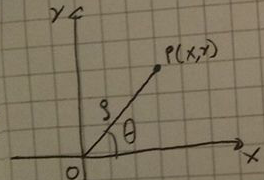
\includegraphics[width=0.5\textwidth]
		{images/coord_pol.png}
		\caption{\label{fig:my-label}}}
\end{figure}

Possiamo definire una curva in \textbf{forma polare} nel seguente modo
\begin{align}
\gamma \, : \, \underline{\rho}=\underline{\rho}(\theta)\in C^1([\theta_1,\theta_2]) \quad , \quad \theta \in [\theta_1,\theta_2]
\end{align}

Intuitivamente viene da scrivere che
\begin{align}
lung(\gamma)= \int_{\theta_1}^{\theta_2} d\theta \, |\rho'(\theta)|
\end{align}

Ma questo è \textbf{SBAGLIATISSIMO}!

\newpage

Bisogna procedere nel seguente modo:
\begin{align}
\left\{
\begin{array}{cc}
x(\theta)=\rho(\theta) \cos(\theta)\\
y(\theta)=\rho(\theta) \sin(\theta)
\end{array}
\right.
\end{align}
Da cui
\begin{align}
|r'(\theta)|^2{}&= [ \rho'(\theta) \cos(\theta) - \rho(\theta) \sin(\theta) ]^2+ [\rho'(\theta) \sin(\theta) + \rho(\theta) \cos(\theta)]^2 = \nonumber \\
&= [\rho'(\theta) \cos(\theta)]^2 - 2\rho'(\theta) \cos(\theta) \rho(\theta) \sin(\theta) + [\rho(\theta) \sin(\theta) ]^2 + \nonumber \\
&+ [\rho'(\theta) \sin(\theta)]^2 + 2\rho'(\theta) \cos(\theta) \rho(\theta) \sin(\theta) + [\rho(\theta) \cos(\theta) ]^2 = \nonumber \\
&= [\rho'(\theta)]^2 [\cos(\theta)^2 + \sin^2(\theta)] + [\rho(\theta)]^2 [\cos(\theta)^2 + \sin^2(\theta)] = \nonumber \\
&= [\rho'(\theta)]^2 + [\rho(\theta)]^2
\end{align}
Questo ci porta ad avere una quantità maggiore di zero solo in caso di curve regolari e ad avere
\begin{align}
|r'(\theta)| = \sqrt{[\rho'(\theta)]^2 + [\rho(\theta)]^2}
\end{align}
Che ci porta alla corretta espressione di lunghezza di una curva in forma polare:
\begin{align}
lung(\gamma)= \int_{\theta_1}^{\theta_2} d\theta \, \sqrt{[\rho'(\theta)]^2 + [\rho(\theta)]^2}
\end{align}

\subsection{Esempi di curve}

\subsubsection{Cicloide}

\begin{align}
\underline{r}(t)=\left\{
\begin{array}{cc}
x(t)= r \, \cdot (t-\sin(t)) \\
y(t)= r \, \cdot (1-\cos(t))
\end{array}
\right. \quad ; \quad t \in [0,2\pi]
\end{align}

Notiamo come le componenti siano ben più che di classe $C^1$ e otteniamo

\begin{align}
{}&\underline{r}'(t)=\left\{
\begin{array}{cc}
x'(t) {}&= r \, \cdot (1-\cos(t)) \\
y'(t) &= r \, \cdot \sin(t) \qquad \;\,\,
\end{array}
\right. \\
\nonumber \\
&|r'(t)|^2= r^2 \, \cdot (1 - 2\cos(t) + \cos^2(t) + \sin^2(t))=2r^2(1-\cos(t))\\
&|r'(t)|^2 >0 \quad \forall t \in (0,2\pi) \\
& |r'(t)|= \sqrt{2} \; r \, \sqrt{1-\cos(t)}
\end{align}

Da cui ricaviamo 

\begin{align}
lung(\gamma)= \sqrt{2} \; r \int_{0}^{2\pi}dt \, \sqrt{1-\cos(t)} = 2r   \int_{0}^{2\pi} dt \, \sin\left(\frac{t}{2}\right) = 8 r
\end{align}

\subsubsection{Ellittica}

\begin{align}
\left(
\frac{x}{a}
\right)^2 + \left(
\frac{y}{b}
\right)^2=1 \quad ; \quad a,b>0
\end{align}

\begin{align}
{}&\underline{r}(t)=\left\{
\begin{array}{cc}
x(t)= a \cos(t) \\
y(t)= b \sin(t)
\end{array}
\right. \quad ; \quad t \in [0,2\pi]\\
&|r'(t)|= [-a \sin(t)]^2 + [b \cos(t)]^2
\end{align}

\begin{align}
lung(\gamma) {}&= \int_{0}^{2\pi} dt \, \sqrt{[-a \sin(t)]^2 + [b \cos(t)]^2} = \nonumber \\
&= \int_{0}^{2\pi} dt \, \sqrt{a^2 [1-\cos^2(t)] + b^2 \cos^2(t)}  = \nonumber \\
&= \int_{0}^{2\pi} dt \, \sqrt{a^2 + (b^2-a^2)\cos^2(t)} = \nonumber \\
&= \int_{0}^{2\pi} dt \, \sqrt{1 + \frac{b^2-a^2}{a^2}\cos^2(t)} = \nonumber \\
&= \int_{0}^{2\pi} dt \, \sqrt{1 + e \cos^2(t)} \quad ; \quad e= \frac{b^2-a^2}{a^2} \quad \text{elliticità}
\end{align}

questi integrali non sono di facile risoluzione e o si trovano tabulati o si approssima.

\subsubsection{Cardioide (curva in forma polare)}

\begin{align}
{}&\rho(\theta)= a[1+\cos(\theta)] \quad ; \quad \theta \in [-\pi, +\pi] \, , \, a>0 \\
&\rho'(\theta)= - a \sin(\theta) \\
&\underline{r}(t)=\left\{
\begin{array}{cc}
x(t)= a[1+\cos(\theta)] \cos(t) \\
y(t)= a[1+\cos(\theta)] \sin(t)
\end{array}
\right. \quad ; \quad t \in [0,2\pi]
\end{align}

Per semplicità poniamo $a=1$ e otteniamo
\begin{align}
lung(\gamma){}&= \int_{-\pi}^{+\pi} d\theta \, \sqrt{\sin^2(\theta) + [1+\cos(\theta)]^2} = \nonumber \\
&= \int_{-\pi}^{+\pi} d\theta \, \sqrt{ 2 + 2 \cos(\theta)}= \nonumber \\
&=\sqrt{2} \int_{-\pi}^{+\pi} d\theta \, \sqrt{ 1 +  \cos(\theta)}= 2 \int_{-\pi}^{+\pi} d\theta \, \left|\cos\left(\frac{\theta}{2}\right)\right|=8
\end{align}


\subsubsection{Spirale logaritmica}
\begin{align}
{}&\rho = \Exp{\theta} \spacer \theta\in[0,2\pi]\\
&\underline{r}(\theta)=\double{x(\theta)= \Exp{\theta}\cos(\theta) }{y(\theta) = \Exp{\theta}\sin (\theta)}\\
& lung(\gamma)= \int_{0}^{2\pi}d\theta \, \sqrt{\Exp{2\theta} + \Exp{2\theta}} = \sqrt{2}\int_{0}^{2\pi}d\theta \, \Exp{\theta}= \sqrt{2}(\Exp{2\theta} -1)
\end{align}

\subsubsection{Spirale di Archimede}

\begin{align}
{}&\rho = \theta \spacer \theta\in[0,\frac{\pi}{6}]\\
&\underline{r}(\theta)=\double{x(\theta)= \theta\cos(\theta) }{y(\theta) = \theta\sin (\theta)}\\
& lung(\gamma)= \int_{0}^{\frac{\pi}{6}}d\theta \, \sqrt{1 + \theta^2} = \int_{0}^{\overline{u}}du \, \cosh^2(u) = \frac{\pi}{2} + \fracn{4}\sinh \left(\frac{\pi}{3}\right)
\end{align}

Abbiamo applicato il seguente cambio di variabile
\begin{align}
{}&\theta = \sinh(u) \implies d\theta = \cosh(u)du \\
&1 + \theta^2= 1 + \sinh^2(u) = \cosh^2(u)
\end{align}


\newpage

\section{Integrali curvilinei}


\subsection{Integrali curvilinei di I tipo (o di funzione)}

Sia una curva regolare 
\begin{align}
\gamma \, : \, \underline{r}(t)=(x(t),y(t),z(t)) \quad ; \quad t \in [a,b]
\end{align}
e sia
\begin{align}
f \, : \, A \subseteq \mathbb{R}^3 {}&\longrightarrow \mathbb{R} \\
(x,y,z) & \longrightarrow f(x,y,z)
\end{align}
quantomeno continua e tale che $(\mathbb{R}^3, ||\cdot||_3) \longrightarrow (\mathbb{R},||\cdot||)$, avremo allora
\begin{align}
\int_{\gamma} ds \, f = \int_{a}^{b} dt \, f(x(t),y(t),z(t))\sqrt{[x'(t)]^2 + [y'(t)]^2 + [z'(t)]^2}
\end{align}
Che ci rappresenta questa quantità? Possiamo dargli due interpretazioni:
\begin{enumerate}
	\item \textbf{Geometrica:}

	\begin{figure}[!htb]
		\center{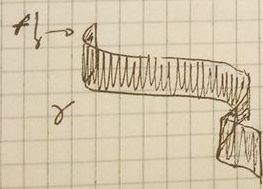
\includegraphics[width=0.5\textwidth]
			{images/int_curv.png}
			\caption{\label{fig:my-label}}}
	\end{figure}
	
	L'integrale misura il "muro" che viene "innalzato" lungo $\gamma$ da $f(x,y,z)$
	
	\item \textbf{Fisica:}

	L'integrale misura la massa di un filo di lunghezza $\gamma$ e densità $f(x,y,z)$ (ha senso se $f(x,y,z)\geq 0$)
\end{enumerate}

Per curve equivalenti $\gamma_1$ $\gamma_2$ si ha che 
\begin{align}
\int_{\gamma_1} ds \, f = \int_{\gamma_2} ds \, f
\end{align}

Con indipendenza dal verso di percorrenza. La dimostrazione di questa proprietà discende direttamente da quella della lunghezza di curve equivalenti.

\textbf{Caso particolare:} la funzione identità restituisce la lunghezza della curva!

Gli integrali curvilinei del Io tipo godono delle seguenti proprietà:

\begin{enumerate}
	\item \textbf{Linearità:
	\begin{align}
	\int_{\gamma} ds \, (\alpha f + \beta g)= \alpha\int_{\gamma} ds \, f + \beta \int_{\gamma} ds \, g
	\end{align}}

	\item \textbf{Monotonia}:
	\begin{align}
	f\leq g \implies \int_{\gamma} ds \, f \leq \int_{\gamma} ds \, g
	\end{align}
	
	\item \textbf{Teorema del modulo:}
	\begin{align}
	\left| \int_{\gamma} ds \, f \right| \leq \int_{\gamma} ds \, |f|
	\end{align}
\end{enumerate}

\newpage

\subsection{Esempi di I.C. di Io tipo}

\begin{enumerate}
	\item $\gamma \taleche x^2 +y^2 =1 \spacer x,y \geq 0 = z$ 
	\begin{align}
	{}&\underline{r}(t)= \double{x(\theta)= \cos(\theta)}{y(\theta) = \cos(\theta)}\spacer \theta \in \left[0,\frac{\pi}{2}\right] \\
	&|r'(t)|= \sqrt{\sin^2(\theta) + \cos^2(\theta)}=1 \spacer ds = |r'(t)|dt=dt\\
	&\int_{\gamma} ds (x + y -1) = \int_{0}^{\frac{\pi}{2}}d\theta ( \cos(\theta) + \sin(\theta) -1)= \dots = 2 - \frac{\pi}{2}
	\end{align}

	\item $\gamma \taleche \underline{r}(t) \triple{x(t)= \cos(t)}{y(t)= \sin(t)}{z(t)=t} \spacer t \in [0,\pi] \implies |r'(t)|= 2 \spacecomma ds = \sqrt{2}dt$
	\begin{align}
	\int_{\gamma} ds (x^2 + y^2 + z^2) {}&= \sqrt{2}\int_{0}^{\pi} dt (1 + t^2) = \sqrt{2} \left[t|_0^\pi + \left.\frac{t^3}{3}\right|_0^\pi \right] = \continue &=\sqrt{2}\left(\pi + \frac{\pi^3}{3}\right)
	\end{align}
	
\end{enumerate}

\subsection{Baricento (o centro di massa) di una curva}

Si definisce \textbf{baricentro} di una curva con densità lineare $f\geq 0$ il punto con coordinate
\begin{align}
{}&x_B=\frac{\int_{\gamma}ds \, x\cdot f}{\int_{\gamma}ds \, f} \\
&y_B=\frac{\int_{\gamma}ds \, y\cdot f}{\int_{\gamma}ds \, f} \\
&z_B=\frac{\int_{\gamma}ds \, z\cdot f}{\int_{\gamma}ds \, f}
\end{align}

\textbf{Nota bene:} non è detto che $(x_B,y_B,z_B)\in\gamma$

Vediamo in pratica di cosa si parla con l'esempio del quarto di asteroide:
\begin{align}
{}&\underline{r}(t)=\left\{
\begin{array}{cc}
x(t)=\cos^3(t)\\
y(t)=\sin^3(t)
\end{array}
\right. \quad ; \quad t\in \left[0,\frac{\pi}{2}\right]\\
&f=1 \quad \text{densità costante}\\
&|r'(t)|= 3 \sin(t)\cos(t) 
\end{align}

	\begin{figure}[!htb]
	\center{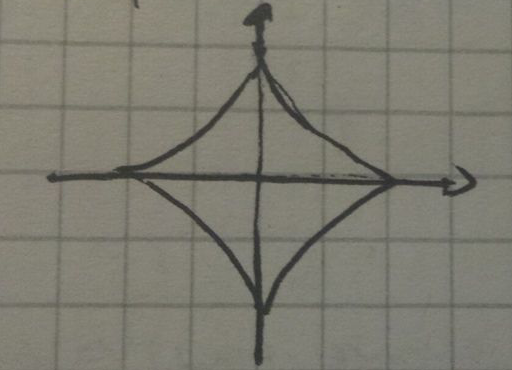
\includegraphics[width=0.4\textwidth]
		{images/asteroide.png}
		\caption{\label{fig:my-label}}}
	\end{figure}
\begin{align}
lung(\gamma){}&= \int_{\gamma}ds \, f = 3 \int_{0}^{\frac{\pi}{2}} dt \, \sin(t)\cos(t)\rightarrow \left\{
\begin{array}{cc}
u=\cos(t)\\
du=\sin(t)dt
\end{array}
\right. \rightarrow 3\int_{0}^{1} du \, u = \nonumber\\
&=\frac{3}{2}u^2|_{0}^{1}=\frac{3}{2}
\end{align}	
\begin{align}
x_B {}&= \int_{\gamma}ds \, x\cdot f = 3 \int_{0}^{\frac{\pi}{2}} dt \, \cos^3(t)\cdot \sin(t)\cos(t) = \nonumber \\
&= \int_{0}^{\frac{\pi}{2}} dt \, \cos^4(t)\sin(t) = \nonumber \\
&= - 3 \int_{1}^{0} du \, u^4 = \frac{3}{5}u^5|_{0}^{1}= \frac{3}{5} \\
\nonumber \\
y_B &= \int_{\gamma}ds \, y\cdot f= 3 \int_{0}^{\frac{\pi}{2}} dt \, \sin^3(t)\cdot \sin(t)\cos(t)=\nonumber \\
&= \dots = \nonumber \\
&= \frac{2}{5}
\end{align}
	
\subsection{Integrali curvilinei di II tipo (o di campo vettoriale)}

Prima di definirli, ci domandiamo: cos'è un campo vettoriale?

È un vettore tale che
\begin{align}
\underline{F}(x,y,z)\, : \, A \subseteq \mathbb{R}^3 {}&\longrightarrow \mathbb{R}^3 \\
(x,y,z) &\longrightarrow (F_1(x,y,z),F_2(x,y,z),F_3(x,y,z)) \nonumber
\end{align}
Le cui componenti sono quantomeno continue.

Supponiamo ora di avere $\gamma\in A$, e definiamo il \textbf{versore tangente} come
\begin{align}
\underline{T}(t)=\frac{(x'(t),y'(t),z'(t))}{\sqrt{[x'(t)]^2 + [y'(t)]^2 + [z'(t)]^2}}
\end{align}

E possiamo infine definire gli \textbf{integrali curvilinei di IIo tipo} come
\begin{align}
\int_{\gamma}ds \, \underline{F}\cdot \underline{T}
\end{align}

Questa quantità ha un significato fisico ben preciso: è il lavoro delcampo di forze $\underline{F}$ per spostare lungo $\gamma$ un corpo puntiforme. Lo indicheremo quindi con $W$.

Operativamente questa definizione è però poco utile, memori quindi di quanto fatto per gli integrali di primo tipo, e svolgendo il prodotto tra i due vettori otteniamo:
\begin{align}
W{}&=\int_{\gamma}ds \, \underline{F}\cdot \underline{T} = \nonumber \\
&= \int_{a}^{b}dt \, \left[F_1(r(t)) \frac{x'(t)}{|r'(t)|} + F_2(r(t)) \frac{y'(t)}{|r'(t)|} + F_3(r(t)) \frac{z'(t)}{|r'(t)|}
\right] |r'(t)|= \nonumber \\
&= \int_{a}^{b}dt \, \left[F_1(r(t)) x'(t) + F_2(r(t)) y'(t) + F_3(r(t)) z'(t)
\right]
\end{align}

\textbf{Nota bene:} Mentre per gli integrali di I tipo per curve equivalenti il risultato era lo stesso anche per versi opposti, in questo caso il verso di percorrenza è rilevante.

\subsubsection{Esempi di Integrali curvilinei di II tipo}

Calcoliamo ora il lavoro di una serie di campi vettoriali.

\begin{enumerate}
	\item $\underline{F}=(1,0,0)$ lungo il segmento $\underline{x_0}=(0,0,0)\longrightarrow \underline{x_1}=(1,2,3)$
	
	L'unica rappresentazione possibile per il segmento sarà:
	
	\begin{align}
		{}&\underline{r}(t)=\left\{
		\begin{array}{ccc}
			x(t) = x_0 + (x_1 - x_0)t\\
			y(t) = y_0 + (y_1 - y_0)t\\
			z(t) = z_0 + (z_1 - z_0)t 
		\end{array}
		\right. \implies
		\underline{r}(t)=\left\{
		\begin{array}{ccc}
			x(t) ={}& \, t\\
			y(t) =& 2t\\
			z(t) =& 3t 
		\end{array}
		\right. \quad ; \quad
		\underline{r}'(t)=\left\{
		\begin{array}{ccc}
			x'(t) ={}& 1\\
			y'(t) =& 2\\
			z'(t) =& 3 
		\end{array}
		\right. \nonumber \\
		\nonumber\\
		&W=\int_{0}^{1} dt \, [1\cdot 1 + 0 \cdot 2 + 0 \cdot 3]= \int_{0}^{1}dt = 1
	\end{align}
	
	\item $\underline{F}=(y \, , \, x^2 + y^2\, , \, 0)=(y\, , \, x^2 + y^2)$ 
	
	lungo l'arco di circ. $x^2 + y^2=4$ con estremi   $\underline{x}_0=(-2,0) \longrightarrow \underline{x}_1=(0,2)$
	
	\begin{align}
		{}& {x}_0=(-2,0) \longrightarrow \underline{x}_1=(0,2) \implies t_0=\pi \longrightarrow t_1=\frac{\pi}{2}\\
		&\underline{r}(t)=\left\{
		\begin{array}{cc}
			x(t)=2\cos(t) \\
			y(t)=2\sin(t)
		\end{array}
		\right. \quad ; \quad
		\underline{r}'(t)=\left\{
		\begin{array}{cc}
			x'(t)=-2\sin(t) \\
			y'(t)=+2\cos(t)
		\end{array}
		\right.
	\end{align}
	\begin{align}
		W {}&= - \int_{\frac{\pi}{2}}^{\pi} dt \, [2\sin(t)\cdot (-2\sin(t)) + 4 \cdot (2\cos(t))] = \nonumber \\
		&=4 \int_{\frac{\pi}{2}}^{\pi} dt \, [\sin(t) -2\cos(t)]= \dots = \pi + 8
	\end{align}
	
	\item \textbf{Il campo gravitazionale:} 
	$\underline{F}=\frac{Gm}{(x^2 + y^2 + z^2)^{\frac{3}{2}}}(x,y,z)$
	
	Data una generica curva $\gamma \, : \, r(t)=(x(t),y(t),z(t))$ con $t\in[a,b]$ contenuta in $A\subseteq \mathbb{R}^3 \backslash\left\{(0,0,0)\right\}$
	
	\begin{align}
		W {}&= -Gm \int_{a}^{b} dt \, \frac{1}{(x^2 + y^2 + z^2)^{\frac{3}{2}}} [x(t)x'(t) + y(t)y'(t) + z(t)z'(t)] = \nonumber \\ 
		&= -Gm \int_{a}^{b} dt \, \frac{d}{dt}\left(\frac{1}{\sqrt{x^2 + y^2 + z^2}}\right)= -Gm \int_{a}^{b} dt \, \frac{d}{dt}\left(\frac{1}{|r(t)|}\right)  = \nonumber \\ 
		&= Gm\left(\frac{1}{|r(b)|} - \frac{1}{|r(a)|}\right)
	\end{align}
	Notiamo l'indipendenza dal percorso ma non dai punti di inizio e fine.
\end{enumerate}

\chapter{Funzioni in $\mathbb{R}^n$}

\section{Limiti di funzioni}

Sia una funzione
\begin{align}
f \, : \, A\subseteq \mathbb{R}^n {}&\longrightarrow \mathbb{R}^m \quad n,m\geq 1\\
\underline{x}=(x_1,\dots,x_n) &\longrightarrow \underline{f}(\underline{x})=(f_1(\underline{x}), \dots , f_n(\underline{x})) \nonumber
\end{align}
e sia $\underline{x}^0 \in acc(A)$, avremo
\begin{align}
\underset{\underline{x} \rightarrow \underline{x}^0}{\lim}\,\underline{f}(\underline{x})=\underline{l}=(l_1,\dots,l_n)\in \mathbb{R}^m
\end{align}
Ma questo implica che
\begin{align}
\underset{x_i\rightarrow x_i^0}{\lim} f_i(x_i)=l_i \quad \forall i =1,\dots,n
\end{align}
e quindi il problema si riduce allo studio dei limiti $l_i \in \mathbb{R}$

\subsection{Limiti in $\mathbb{R}$}

Siano $\underline{f} \, : \, A\subseteq \mathbb{R}^n \longrightarrow \mathbb{R}$ e $\underline{x}^0 \in acc(A)$, si definisce il \textbf{limite} di $\underline{f}$ ad $\underline{x}^0$ come:
\begin{align}
{}&\underset{\underline{x}\rightarrow\underline{x}^0}{\lim}f(\underline{x})=l \in \mathbb{R}\cup \left\{\pm \infty \right\}\\ 
&\updownarrow \nonumber \\ 
&\forall U(l) \; \exists I_\delta(\underline{x}^0) \, : \, f(\underline{x}) \in U(l) \quad \forall \underline{x}\in I_\delta(\underline{x}^0)\backslash\left\{\underline{x}^0\right\}\\ 
&\updownarrow \nonumber \\ 
&\forall \epsilon>0 \, \exists \delta_\epsilon \, : \, |f(\underline{x}) - l|_1<\epsilon \quad \forall \underline{x}\in A \, : \, |\underline{x} - \underline{x}^0|_n\leq \delta_\epsilon
\end{align}

\textbf{Nota bene:} Tutti i teoremi per i limiti validi in $\mathbb{R}$ lo sono anche per $\mathbb{R}^n$.

\section{Funzioni continue in $\mathbb{R}^n$}

Si parla di \textbf{continuità in un punto} $\underline{x}^0\in A$ quando 
\begin{align}
\exists \underset{\underline{x}\rightarrow\underline{x}^0}{\lim} \, f(\underline{x})= f(\underline{x}^0)
\end{align} 
e di \textbf{continuità in tutto l'insieme} $A$ quando vale $\forall x\in A$.

\subsection{Connessione}

Si dice che un insieme $A$ è connesso se $\nexists A_1,A_2$ tali che
\begin{enumerate}
	\item $A_1\neq \emptyset \neq A_2$
	\item $A_1\cap A_2=\emptyset$
	\item $A= A_1\cup A_2$
\end{enumerate}

\subsection{Teoremi sulle funzioni continue}

Enunciamo senza dimostrazione alcuni teoremi utili sulle funzioni continue:
\begin{enumerate}
	\item \textbf{Primo teorema:}
	
	\textit{$f$ è continua se e solo se $\forall \underset{aperto}{E} \in \mathbb{R}$ si ha che $f^{-1}(E)$ è aperto}
	
	\item \textbf{Teorema di Weierstrass:}
	
	\textit{Sia $f$ continua in $D\subset \mathbb{R^n}$ chiuso e limitato (compatto), allora $f$ ammette massimo e minimo in $D$ tali che}
	\begin{align}
	{}&x_m \, : \, f(x_m)=\underset{x\in D}{min}f(x)\leq f(x) \quad \forall x \in D \\
	&x_M \, : \, f(x_M)=\underset{x\in D}{max}f(x)\geq f(x) \quad \forall x \in D
	\end{align}
	
	\item \textbf{Teorema dell'esistenza dei valori intermedi:}
	
	\textit{Siano $f \, : \, D\subset \mathbb{R}^2 \longrightarrow \mathbb{R}$ continua e $D$ chiuso, limitato e connesso.}
	
	\textit{Allora $f$ assume tutti i valori possibili tra il suo massimo e il suo minimo.}
\end{enumerate}

\section{Funzioni in $\mathbb{R}^2$}

Studiamo ora un categoria di funzioni in $\mathbb{R}^n$ molto specifica, le funzioni in $\mathbb{R}^2$, ovvero tali che
\begin{align}
f \, : \, A\subseteq \mathbb{R}^2 {}&\longrightarrow \mathbb{R} \\
(x,y) &\longrightarrow f(x,y) \nonumber
\end{align}

Chiamiamo \textbf{Grafico} di una funzione il seguente insieme:
\begin{align}
\{(x,y,z) \, : \, (x,y)\in D \, ; \, z=f(x,y)\}
\end{align}

E chiamiamo \textbf{curve (o linee) di livello}:
\begin{align}
\{ (x,y) \in D \, : \, f(x,y)=cost. \}
\end{align}

\subsubsection{Esempi di calcolo dell'insieme di definizione}

\begin{enumerate}
	\item $f(x,y)=\sqrt{4-x^2-y^2} \implies D= \{ (x,y) \, : \, x^2 + y^2 \leq 4 \}$
	
	\item $f(x,y)=\ln(4-x^2-y^2) \implies D= \{ (x,y) \, : \, x^2 + y^2 < 4 \}$
\end{enumerate}

\subsubsection{Funzioni radiali}

Sono una categoria di $f\in \mathbb{R}^2$ del tipo

\begin{align}
f(x,y)=f(\sqrt{x^2 + y^2})
\end{align}

che possono essere quindi espresse come funzioni di una sola variabile.

Le linee di livello di queste funzioni possono essere solo circonferenze.

Un esempio di funzione radiale è scritto poco sopra, infatti

 $f(x,y)=\sqrt{4-x^2-y^2} = \sqrt{4-t^2}=f(t=\sqrt{x^2 + y^2})$
 
\newpage
 
\subsection{Calcolo dei limiti}
 
 Iniziamo dando nuovamente la definizione di limite:
  \begin{align}
 {}&\underset{\underline{p}\rightarrow \underline{p}_0}{\lim} f(x,y)=l\in \mathbb{R} \\ 
 &\updownarrow \nonumber\\
 &\forall \epsilon >0 \quad \exists \delta_\epsilon>0 \, : \, |f(x,y)-l|<\epsilon \quad \forall (x_0,y_0) \, : \, d(\underline{p},\underline{p}_0)<\delta_\epsilon \\
 &\left\{
 \begin{array}{cc}
 &\underline{p}=(x,y) \quad ; \quad \underline{p}_0=(x_0,y_0) \\
 &d(\underline{p},\underline{p}_0)=\sqrt{(x-x_0)^2 + (y-y_0)^2}\\
 \end{array} 
 \right.
 \end{align}
 
 Il calcolo dei limiti in più dimensione è una questione molto più complicata rispetto a quelli in una sola. 
 
 Infatti affinché esista un limite, la funzione vi teve tendere da tutte le infinite direzioni e traiettorie possibili! (e quindi non solo dalle rette parallele agli assi, per esempio).
 
 Come procediamo allora?
 
 Innanzitutto dobbiamo trovare un \textbf{candidato limite}, che \underline{potrebbe} (ma \underline{non è detto} che sia) il valore da noi cercato.
 
  Dato un punto $(x_0,y_0)$ possiamo utilizzare due metodi:
 
 \begin{enumerate}
 	\item \textbf{Limite lungo le parallele agli assi}:
 	\begin{align}
 	l_x = \underset{x\rightarrow x_0}{\lim} f(x,y_0) \\
 	l_x = \underset{y\rightarrow y_0}{\lim} f(x_0,y) 
 	\end{align}
 	se $l_x=l_y$ abbiamo un candidato limite valido (ma non è detto sia il limite!), altrimenti possiamo fermarci subito.
 	
 	\item \textbf{Limite lungo una curva $\gamma$:}
 	\begin{align}
 	{}&\underline{r}(t) = \left\{
 	\begin{array}{cc}
 	x=x(t)\\
 	y=y(t)
 	\end{array}
 	\right. 	\quad ; \quad \left\{
 	\begin{array}{cc}
 	x_0=x(t_0)\\
 	y_0=y(t_0)
 	\end{array}
 	\right. \\
 	&\underset{t\rightarrow t_0}{\lim}f(x(t),y(t))=l_\gamma
 	\end{align}
 	
 	Anche qui, se troviamo due curve $\gamma_1$ e $\gamma_2$ tali che $l_{\gamma_1} \neq l_{\gamma_2}$ possiamo interrompere subito la ricerca.
 \end{enumerate}

Vediamo alcuni esempi calcolabili con le scarse conoscenze al momento in nostro possesso:
\begin{enumerate}
	\item $\underset{\underline{p}\rightarrow \underline{p}_0}{\lim} \frac{x^2}{\sqrt{x^2 + y^2}} \quad ; \quad \underline{p}_0=(0,0) \quad ; \quad  x\in A=\mathbb{R}^2\backslash \{\underline{p}_0\}$
	
	\bigskip
	Cerchiamo un candidato limite col primo metodo:
	\begin{align}
	{}&\underset{x\rightarrow x_0}{\lim}f(x,0)= \underset{x\rightarrow x_0}{\lim} \frac{x^2}{\sqrt{x^2}}= \underset{x\rightarrow x_0}{\lim} |x| = 0\\
	&\underset{y\rightarrow y_0}{\lim}f(0,y)= \underset{x\rightarrow x_0}{\lim} \frac{0}{\sqrt{y^2}}= 0
	\end{align}
	
	Abbiamo quindi un candidato in $l=0$.
	
	Applichiamo la definizione di limite:
	\begin{align}
	\left|\frac{x^2}{\sqrt{x^2 + y^2}}-0\right| = \frac{x^2}{\sqrt{x^2 + y^2}}\leq \frac{x^2 + y^2}{\sqrt{x^2 + y^2}}=\sqrt{x^2 + y^2}
	\end{align}
	
	Abbiamo maggiorato $x^2$ con $x^2 + y^2$.
	
	Notiamo come $\sqrt{x^2 + y^2}$ nella def. di limite deve essere $<\delta_\epsilon$, e quindi avremo
	
	\begin{align}
	\left|\frac{x^2}{\sqrt{x^2 + y^2}}-0\right|< \delta_\epsilon=\epsilon \quad \forall (x,y) \, : \, \sqrt{x^2 + y^2}<\delta_\epsilon
	\end{align}
	
	E quindi $0$ è effettivamente il limite.
	
	\item $\underset{\underline{p}\rightarrow \underline{p}_0}{\lim} \frac{x}{\sqrt{x^2 + y^2}} \quad ; \quad \underline{p}_0=(0,0) \quad ; \quad  x\in A=\mathbb{R}^2\backslash \{\underline{p}_0\}$
	
	\bigskip
	In questo caso, procedendo col primo metodo avremo:
	\begin{align}
	{}&\underset{x\rightarrow x_0}{\lim}f(x,0)= \underset{x\rightarrow x_0}{\lim} \frac{x}{\sqrt{x^2}}= \underset{x\rightarrow x_0}{\lim} \frac{1}{|x|} = +\infty\\
	&\underset{y\rightarrow y_0}{\lim}f(0,y)= \underset{x\rightarrow x_0}{\lim} \frac{0}{\sqrt{y^2}}= 0
	\end{align}
	
	E vediamo già che $l_x\neq l_y$ e quindi fermiamo subito la ricerca.
	
	\item $\underset{\underline{p}\rightarrow \underline{p}_0}{\lim} \frac{x-y}{x + y} \quad ; \quad \underline{p}_0=(0,0) \quad ; \quad  x\in A=\mathbb{R}^2\backslash \{x=y\}$
	
	\bigskip
	
	Con il primo metodo troviamo
	\begin{align}
	&\underset{x\rightarrow x_0}{\lim}f(x,0)= \underset{x\rightarrow x_0}{\lim} \frac{x}{x}= +1\\
	&\underset{y\rightarrow y_0}{\lim}f(0,y)= \underset{x\rightarrow x_0}{\lim} \frac{y}{-y}= -1
	\end{align}
	
	e quindi buca, visto che $l_x\neq l_y$
	
	Vediamo come anche col secondo metodo non si abbia limite:
	
	Prendendo tutte le rette possibili con $y=mx$
	\begin{align}
	y=mx \implies f(x,mx)=\frac{x + mx}{x - mx}= \frac{1+m}{1-m}
	\end{align}
	
	Abbiamo qualcosa dipendente da una variabile, e quindi infiniti possibili risultati, mentre il limite deve essere unico per tutte le direzioni.
	
	\item $\underset{\underline{p}\rightarrow \underline{p}_0}{\lim}\frac{x^2 y^2}{x^2 + y^2}  \quad ; \quad \underline{p}_0=(0,0) \quad ; \quad  x\in A=\mathbb{R}^2\backslash \{\underline{p}_0\}$
	
	\bigskip
		
	è evidente come $f(0,y)=0=f(x,0)$ e come
	
	 $f(x,mx)=\frac{m^2 x^2}{1+m^2}\overset{x\rightarrow 0}{\longrightarrow} 0$
	
	E quindi con entrambi i metodi si trova un candidato in $l=0$
	
	Applicando la definizione di limite si trova
	\begin{align}
	0\leq \left|\frac{x^2 y^2}{x^2 + y^2} - 0\right|= \frac{x^2 y^2}{x^2 + y^2}\leq x^2 + y^2 < \delta^2_\epsilon
	\end{align}
	
	E facendo discorsi analoghi all'esempio 2 possiamo dire che $l=0$ è proprio il nostro limite.
\end{enumerate}

\subsubsection{Calcolo dei limiti in forma polare} 

Un comodo metodo per risolvere i limiti è quello di lavorare in coordinate polari nel seguente modo:

\begin{align}
&\left\{
\begin{array}{cc}
x=x_0 + \rho \cos(\theta)\\
y=y_0 + \rho \sin(\theta)
\end{array}
\right. \\
&\downarrow \nonumber \\
&|f(\rho \cos(\theta),\rho \sin(\theta)) - l|<\epsilon \leftrightarrow \rho \in [0,\delta_\epsilon] \quad \forall \theta \in [0,2\pi]
\end{align}
Questo implica anche che
\begin{align}
{}&s(\rho)= \underset{\theta}{sup}|f(\rho \cos(\theta),\rho \sin(\theta)) - l|<\epsilon \leftrightarrow \rho \in [0,\delta_\epsilon] \quad \forall \theta \in [0,2\pi]\\
&s(\rho)\geq 0
\end{align}
E quindi avremo che 
\begin{align}
\underset{\rho \rightarrow 0}{\lim}s(\rho)=0 \leftrightarrow \underset{\underline{p}\rightarrow \underline{p}_0}{\lim}f(x,y)=l
\end{align}
E ci basta maggiorare $s(\rho)$ con quantità infinitesime non dipendenti da $\theta$ per verificare che il candidato $l$ è effettivamente il limite cercato.

\bigskip

Vediamo un \textbf{esempio operativo:} $\underset{\underline{p}\rightarrow \underline{p}_0}{\lim}\frac{x^4 + y^4}{x^2 + y^2}=? \quad ; \quad \underline{p}_0=(0,0)$

Con il primo metodo troviamo subito un candidato in $l=0$

passiamo in coordinate polari e avremo
\begin{align}
{}&0\leq \frac{\rho^4(\cos^4(\theta) + \sin^4(\theta)) }{\rho^2}= \rho^2(\cos^4(\theta) + \sin^4(\theta)) \leq \rho^2 (1+1)=2\rho^2\\
&\underset{\rho \rightarrow 0}{\lim}\rho^2=0 \implies \underset{\underline{p}\rightarrow \underline{p}_0}{\lim}\frac{x^4 + y^4}{x^2 + y^2}=0
\end{align}

\textbf{Nota 1:}Abbiamo maggiorato sia $\cos^4(\theta)$ che $\sin^4(\theta)$ con $1$, che non dipende da $\theta$.

\textbf{Nota 2:} potevamo procedere anche senza questo metodo maggiorando il denominatore con $x^2 + y^2$ e applicando la definizione di limite come in esempi precedenti.

\subsubsection{Esempi di calcolo di limiti}

\begin{enumerate}
	\item $\limit{\underline{x}}{\underline{x}^0} \frac{xy}{x^2 +y^2}=? \quad ; \quad \underline{x}^0=(0,0)$
	
	Col primo metodo troviamo che $f(0,y)=f(x,0)=0\doubteq l$
	
	Passiamo in coordinate polari
	
	\begin{align}
	\limit{\rho}{0}\frac{\rho^3 \sin(\theta)\cos^2(\theta)}{\rho^2(\rho^2 \cos^4(\theta) + \sin^2(\theta)}= 	\limit{\rho}{0}\frac{\rho \sin(\theta)\cos^2(\theta)}{\rho^2 \cos^4(\theta) + \sin^2(\theta)}=0 \quad \forall \theta
	\end{align}
	Ma questo non basta, dovremmo maggiorare il suo sup, ma non abbiamo modo di dimostrarlo. Se invece studiamo il limite lungo la curva $y=x^2$ troviamo che
	\begin{align}
	\limit{x}{0} \frac{x^4}{x^4 + x^4}= \frac{1}{2}\neq 0
	\end{align}
	e quindi in $(0,0)$ non esiste limite.
	
	\item $\limit{\underline{x}}{\underline{x}^0} \frac{x^2 + y^2}{y}=? \spacer y\neq 0$
	
	Col primo metodo troviamo $l\doubteq 0=f(0,y)$
	
	Proviamo a muoverci lungo la famiglia di rette $y=mx$
	\begin{align}
	f(x,mx)=\frac{(1+m^2)x^2}{mx}=\frac{1+m^2}{m}x\overset{x\rightarrow 0}{\longrightarrow}0 
	\end{align}
	Di nuovo, questo non vuol dire nulla, potremmo avere una qualche curva che da risultati diversi. 
	
	Passiamo in coordinate polari
	\begin{align}
	\limit{\rho}{0} \frac{\rho^2}{\rho \sin(\theta)} = 	\limit{\rho}{0} \frac{\rho}{\sin(\theta)}=0
	\end{align}
	

	Ma anche questo \underline{non basta}! Infatti dobbiamo vedere come si comporta $s(\rho)$, che stavolta possiamo stimare:
	\begin{align}
	s(\rho)= sup\left|\frac{\rho}{\sin(\theta)}\right|=\infty \neq 0
	\end{align}
	
	E quindi nonostante finora sembrasse tutto ok, il limite non esiste. 
	
	Inoltre, volendo ulteriori conferme, provando con la parabola $y=x^2$ troviamo $l_\gamma=1\neq 0$.
	
	\item $f(x,y)=\frac{\sin(2(x-y))}{x-y}$

	Esiste il limite a $(1,1)$?
	
	Iniziamo notando che questa funzione appartiene ad una categoria particolare di funzioni, quelle che possono essere riscritte come funzioni di una variabile:
	\begin{align}
	{}&g(x,y)=x-y = (x-1) + (y-1) \arrowlim{(x,y)}{(1,1)} 0\\
	&g(t)=t=x-y\\
	&f(t)=\frac{\sin(2t)}{t}=\frac{2}{2}\frac{\sin(2t)}{t}=2\frac{\sin(2t)}{2t} \arrowlim{t}{0} 2 	
	\end{align}

	\textbf{Nota bene:} Le funzioni radiali rientrano in questa categoria a pieno titolo, ma allora passando in coordinate polari si avrà che non c'è dipendenza da $\theta$, ciò implica che anche il $sup$ tenderà alla stessa quantità implicando infine l'unicità del limite, riducendo il problema dei limiti di funzioni radiali a 
	\begin{align}
	\limit{\underline{x}}{\underline{x}^0}f(\underline{x})=\limit{\rho}{0}F(\rho) 
	\end{align}
	
	\item $f(x,y)=\Exp{-\frac{1}{x^2 + y^2}} \spacer \R^2\except{(0,0)}$
	
	$f(x,y)$ è chiaramente radiale, quindi possiamo scrivere $f(\rho)=\Exp{-\frac{1}{\rho^2}}$ e avere
	
	\begin{align}
	\limit{\vecx}{\vecx^0}f(\vecx)=\limit{\rho}{0}\Exp{-\frac{1}{\rho^2}}=0
	\end{align}
	
	In casi come questo si dice che la funzione è \textbf{prolungabile per continuità} al punto in questione e si ha la funzione
	
	\begin{align}
	\hat{f}(x,y)= \double{f(x,y) \quad {}&(x,y)\in\R^2 \backslash \{(0,0)\}}{0 \quad &(x,y)=0}
	\end{align}
	
	\item $f(x,y)= \double{g(x,y)=\frac{xy}{x^2 + y^2}\sin^\alpha(|x| + |y|) \quad {}& (x,y)\in \R^2\except{(0,0)}}{0 \quad &(x,y)=(0,0)}$
	
	Ci chiediamo per quali valori di $\alpha$ la funzione è continua. Avremo tre casi:
	
		\begin{enumerate}
			\item $\alpha = 0 \implies g(x,y)=\frac{xy}{x^2 + y^2}$
			
			\smallskip
			
			In questo caso abbiamo già visto come non esista il limite
			
			\smallskip
						
			\item $\alpha < 0 \implies g(x,y)=\frac{xy}{x^2 + y^2} \frac{1}{\sin^{|\alpha|}(|x| + |y|)}$
			
			\smallskip
			
			Vediamo subito come per la retta $y=x$ si abbia
			
			\begin{align}
			{}&g(x,x)= \frac{x^2}{x^2 + x^2} \frac{1}{\sin^{|\alpha|}(|x|+|x|)}=\frac{1}{2} \frac{1}{\sin^{|\alpha|}(2|x|)}\\
			&\limit{x}{0}\frac{1}{2} \frac{1}{\sin^{|\alpha|}(2|x|)}=+\infty\neq 0
			\end{align}
			
			e quindi anche qui non c'è limite
			
			\item $a>0 \implies g(x,y)= \frac{xy}{x^2 + y^2}\sin^{|\alpha|}(|x| + |y|)$
			
			\smallskip
			
			Notiamo come $\frac{|xy|}{x^2 + y^2}\leq \half \implies (|x| - |y|)^2 \geq 0$
			
			E possiamo quindi scrivere, ricordando che $|\sin(x)|\leq |x|$
			
			\begin{align}
			0\leq |f(x,y)-0| {}&\leq \half |sin(|x|+|y|)|^\alpha \leq \half (|x|+|y|)^\alpha \leq \continue
			&\leq \half (2\sqrt{x^2 + y^2})^\alpha = \continue 
			&=2^{\alpha-1}\sqrt{x^2 + y^2}\arrowlim{(x,y)}{(0,0)} 0
			\end{align}
			
			Per il teorema del confronto il limite è dunque $0$ e quindi per $\alpha>0$ la funzione è continua
						\end{enumerate}
\end{enumerate}

\newpage

\subsection{Funzioni derivabili}

Vediamo ora come si estende il concetto di derivabilità alle funzioni 
\begin{align}
f \taleche A \subseteq \R^n \longrightarrow \R
\end{align}

\subsubsection{Derivate Parziali e derivabilità}

Si dice che $f(\vecx)$ è dotata in $\vecx^0 \in A$ di \textbf{derivata parziale} rispetto a $x_i$ se esiste finito
\begin{align}
\limit{h}{0} \frac{f(x^0_1 \spacecomma \dots \spacecomma x^0_{i-1} \spacecomma x^0_i + h \spacecomma x^0_{i+1} \spacecomma \dots,x^0_n)}{h}=\left. \partialder{f}{x_i} \right|_{\vecx^0}
\end{align}
Altre notazioni equivalenti sono $f_{x_i}(\vecx^0) \spacecomma \partial_{x_i}f(\vecx^0)$.

\smallskip

\textbf{In parole povere:} si fissano tutte le variabili tranne una e si procede come nel caso di funzioni in $\R$.  

\bigskip

Qualora $f(\vecx)$ ammetta derivate parziali $\forall x_i$ si dice che la funzione è \textbf{derivabile}  in $\vecx^0$, e in tal caso possiamo anche definire il \textbf{gradiente} della funzione nel punto come
\begin{align}
grad(f(\vecx^0))= \nabla f(\vecx^0)=(f_{x_1}(\vecx^0) \spacecomma \dots \spacecomma f_{x_n}(\vecx^0))
\end{align}

Vediamo ora alcuni \textbf{esempi:}

\begin{enumerate}
	\item $f(x,y)=x^3\sin(y) \spacer \vecx \in \R^2 \implies \vecx=(x,y)$
	
	Questa funzione è derivabile? Assolutamente sì:
	\begin{align}
	{}&f_x(x,y)= 3x^2\sin(y)\\
	&f_y(x,y)=x^3 \cos(y)
	\end{align}
	
	\item $f(x,y)=\double{\frac{x^2 y}{x^2 + y^2} \quad {}& (x,y)\neq (0,0)}{0 \quad &(x,y)=(0,0)}$
	
	\smallskip
	
	il problema qui va diviso in due parti:
	
	\begin{enumerate}
		\item $(x,y) \neq (0,0)$
		
		Il denominatore non si annulla mai e si trovano facilmente entrambe le derivate parziali
		
		\item $(x,y) = (0,0)$
		
		In questo caso applichiamo la definizione:
		\begin{align}
		{}&f_x(0,0)= \limit{h}{0} \frac{f(h,0) - f(0,0)}{h}= \limit{h}{0} \fracn{h} \cdot \frac{h^2 \cdot 0}{h^2 + 0}=0\\ 
		&f_y(0,0)= \limit{k}{0} \frac{f(0,k) - f(0,0)}{k}= \limit{k}{0} \fracn{k} \cdot \frac{0 \cdot k}{k^2 + 0}=0
		\end{align}
		E quindi la funzione ammette derivate parziali in $(0,0)$.
		
		\smallskip
	\end{enumerate}

	\item $f(x,y) = \sqrt{x^2 + y^2}$ è derivabile in $\veczero=(0,0)$?
	\begin{align}
	{}&f_x(\veczero)=\limit{h}{0}\frac{\sqrt{h^2 +0} - 0}{h}= \limit{h}{0} |h|\\
	&f_y(\veczero)=\limit{k}{0}\frac{\sqrt{0+k^2} - 0}{k}= \limit{k}{0} |k|
	\end{align}
	Nessuno dei due limiti esiste, quindi niente derivabilità in $\veczero$.

	\item $f(x,y)=\double{\frac{xy}{x^2 + y^2} \quad {}&(x,y)\neq (0,0)}{0 \quad &(x,y)=(0,0)}$

	Ci troviamo di fronte ad una grande differenza rispetto all'analisi in $\R$: questa funzione, come abbiamo già visto in un precedente esempio, \textbf{non è continua}. 

	Ma se andiamo a studiarne la derivabilità troviamo che:
	\begin{align}
	{}&f_x(\veczero) = \limit{h}{0} \frac{0}{h^2 + 0} \fracn{h}=0 \\
	&f_y(\veczero) = \limit{k}{0} \frac{0}{0+k^2} \fracn{k}=0
	\end{align}
	E quindi ci accorgiamo di come in $\R^n$ per $n\geq 2$ la derivabilità \textbf{non implica} la continuità!
	
\end{enumerate}

\subsubsection{Derivate direzionali}

Le derivate parziali da sole sono riduttive, in quanto studiano l'andamento delle funzioni solo lungo le parallele agli assi. Per avere una visione complessiva dobbiamo introdurre le \textbf{Derivate Direzionali}.

\smallskip

Si dice che $f \taleche A \subseteq\R^n \longrightarrow \R$ è dotata in $\vecx^0 \in A$ di derivata direzionale lungo la direzione individuata dal versore $\hat{v}$ se esiste finito
\begin{align}
\limit{t}{0}\frac{f(\vecx^0 + t \hat{v}) - f(\vecx^0)}{t}= \left. \partialder{f}{\hat{v}} \right|_{\vecx^0} = D_{\hat{v}}f(\vecx^0)
\end{align}

Notiamo come il concetto di derivata direzionale inglobi quello di derivata parziale, che altro non è che una derivata direzionale calcolata lungo una direzione parallela ad uno degli assi.

L'espressione diventa meno criptica se mostriamo il caso particolare che più interessa a noi : $\R^2$
\begin{align}
D_{\hat{v}}f(x_0,y_0)=\limit{t}{0}\frac{f(x_0 + t v_x\spacecomma y_0 + t v_y)-f(x_0,y_0)}{t}
\end{align}

Vediamone ora un \textbf{esempio}:
\begin{align}
f(x,y)=\double{\frac{x^2 y}{x^4 + y^2} \quad {}& \vecx \neq \veczero}{0 \quad &\vecx = \veczero}
\end{align}

Avremo derivate direzionali lungo tutte le possibili direzioni?
\begin{align}
\limit{t}{0} \frac{f(tv_x,tv_y) - f(0,0)}{t} {}&=\limit{t}{0}\fracn{t}\frac{(tv_x)^2 tv_y}{(t v_x)^4 + (tv_y)^2}= \limit{t}{0} \frac{v_x^2 v_y}{t^2 v_x^4 + v_y^2} = \continue
&= \frac{v_x^2}{v_y}
\end{align}

Questo risultato vale solo per $v_y \neq 0$, mentre per $v_y = 0$ avremo
\begin{align}
\limit{t}{0} \frac{f(tv_x,0) - f(0,0)}{t}= \limit{t}{0} \fracn{t} \frac{0}{(tv_x)^4}=0
\end{align}
e quindi complessivamente
\begin{align}
\exists \derdir f(\veczero)= \double{\frac{v_x^2}{v_y} \quad {}&v_y \neq 0}{0 \quad &v_y=0}
\end{align}

Notiamo che anche questa funzione non è continua, e che quindi anche per le derivate direzionali vale il discorso fatto sulla derivabilità in $\R^n$ con $n \geq 2$

\newpage

\subsection{Differenzialibità}

Si dice che una funzione $f \taleche A \subseteq \R^n \longrightarrow \R$ è \textbf{differenziabile} in $\vecx^0 \in A$ se, definito
\begin{align}
R(\vecx,\vecx^0)= f(\vecx) - f(\vecx^0) - \braket{a|X} \spacer \underline{X}=\vecx - \vecx^0
\end{align}
si ha che $\exists \underline{a} \in \R^n \taleche$
\begin{align}
\limit{\vecx}{\vecx^0} \frac{R(\vecx,\vecx^0)}{|\vecx - \vecx^0|_n}=0 \leftrightarrow R(\vecx,\vecx^0)= o(|\vecx - \vecx^0|_n) \quad \text{per} \quad \vecx \rightarrow \vecx^0
\end{align}

\subsubsection{Teoremi sulle funzioni differenziabili}

\begin{enumerate}
	\item \textbf{Primo teorema: Differenzialibità e Continuità}
	
	\textit{Se $f(\vecx)$ è differenziabile in $\vecx^0$ allora è anche continua in quel punto.}
	
	\bigskip
	la dimostrazione procede nel seguente modo:
	\begin{align}
	{}&R(\vecx,\vecx^0)= o(|\vecx - \vecx^0|_n) \implies \limit{\vecx}{\vecx^0}R(\vecx,\vecx^0)= 0\\
	&\underline{X}= \vecx - \vecx^0 \implies \limit{\vecx}{\vecx^0} \underline{X}=0 \implies \limit{\vecx}{\vecx^0} \braket{a|X}=0
	\end{align}
	Questo significa che
	\begin{align}
	\limit{\vecx}{\vecx^0}R(\vecx,\vecx^0) = \limit{\vecx}{\vecx^0} (f(\vecx) - f(\vecx^0) - \cancel{\braket{a|X}})=0
	\end{align}
	Da cui segue la definizione di continuità $\limit{\vecx}{\vecx^0}f(\vecx)=f(\vecx^0)$
	
	
	\item \textbf{Secondo teorema: Differenzialibità e Derivabilità}
	
	\textit{Se $f(\vecx)$ è differenziabile in $\vecx^0$ allora è anche derivabile in quel punto, e si avrà:}
	\begin{align}
	\underline{a}=\nabla f(\vecx^0) \spacer a_i = f_{x_i}(\vecx^0) \quad \forall i
	\end{align}
	
	\bigskip
	la dimostrazione procede nel seguente modo:
	
	Fissiamo tutte le variabili tranne una e calcoliamo il rapporto incrementale:
	\begin{align}
	{}&\limit{x_1}{x_1^0}\frac{f(x_1\spacecomma x_2^0\spacecomma \dots \spacecomma x_n^0) - f(\vecx^0) - \braket{a|X}}{|x_1 - x_1^0|}=\limit{x_1}{x_1^0} \frac{R(x_1\spacecomma x_2^0\spacecomma \dots \spacecomma x_n^0, \spacecomma \vecx^0)}{|x_1 - x_1^0|}= 0 \nextpassage
	& \limit{x_1}{x_1^0}\frac{f(x_1\spacecomma x_2^0\spacecomma \dots \spacecomma x_n^0) - f(\vecx^0) - \braket{a|X}}{|x_1 - x_1^0|} \cdot \frac{x_1 - x_1^0}{x_1 - x_1^0} = 0 \nextpassage
	& \limit{x_1}{x_1^0}\frac{f(x_1\spacecomma x_2^0\spacecomma \dots \spacecomma x_n^0) - f(\vecx^0) - \braket{a|X}}{x_1 - x_1^0} \cdot \frac{x_1 - x_1^0}{|x_1 - x_1^0|} = 0
	\end{align}
	Siccome $\frac{x_1 - x_1^0}{|x_1 - x_1^0|}$ può assumere solo i valori $\pm 1$, segue che deve essere
	\begin{align}
	{}&\limit{x_1}{x_1^0}\frac{f(x_1\spacecomma x_2^0\spacecomma \dots \spacecomma x_n^0) - f(\vecx^0) - \braket{a|X}}{x_1 - x_1^0}=0 \nextpassage
	&\limit{x_1}{x_1^0}\frac{f(x_1\spacecomma x_2^0\spacecomma \dots \spacecomma x_n^0) - f(\vecx^0)}{x_1 - x_1^0} = \frac{\braket{a|X}}{x_1 - x_1^0}
	\end{align}
	Notando come $\frac{\underline{X}}{x_1 - x_1^0}$ altro non sia altro che il versore di lungo la direzione di $x_1$ e quindi
	\begin{align}
	\frac{\braket{a|X}}{x_1 - x_1^0}=a_i
	\end{align}
	come $x_1=x_1^0 + h$ otteniamo il risultato cercato
	\begin{align}
	{}&\limit{h}{0}\frac{f(x_1^0 + h \spacecomma x_2^0\spacecomma \dots \spacecomma x_n^0) - f(\vecx^0)}{h} = a_i \implies a_i = f_{x_i}(\vecx^0)
	\end{align}
	
	\item \textbf{Terzo teorema: Differenzialibità e Derivate Direzionali}
	
	\textit{Se $f(\vecx)$ è differenziabile in $\vecx^0$ allora è anche dotata di derivate direzionali in quel punto, che possono essere espresse come:}
		\begin{align}
	\left. \partialder{f}{\hat{v}}\right|_{\vecx^0}= \braket{\nabla f(\vecx^0)|v}=f_{x_1}(\vecx^0) \cdot v_1 + \dots + f_{x_n}(\vecx^0) \cdot v_n
	\end{align}
	\textbf{Nota bene:} Se f non è continua o derivabile in $\vecx^0$ allora sicuro non è nemmeno differenziabile.
	
	\bigskip
	la dimostrazione procede nel seguente modo:
	
	Abbiamo visto come per funzioni differenziabili sia vero il limite
	\begin{align}
	\limit{\vecx}{\vecx^0}\frac{f(\vecx_n) - f(\vecx^0) - \braket{a|X}}{|\vecx - \vecx^0|_n}  = 0
	\end{align}
	Poniamo ora $\vecx=\vecx^0 + t\hat{v}$ e avremo che $|\vecx - \vecx^0|_n=|t|$ e quindi il limite diventa
	\begin{align}
	&\limit{t}{0} \frac{f(\vecx^0 + t\hat{v}) - f(\vecx^0 ) - \braket{a|v}t}{|t|}=0 \nextpassage
	&\limit{t}{0} \frac{f(\vecx^0 + t\hat{v}) - f(\vecx^0 ) - \braket{a|v}t}{|t|} \cdot \frac{t}{t}=0 \nextpassage
	&\limit{t}{0} \left(\frac{f(\vecx^0 + t\hat{v}) - f(\vecx^0 )}{t} - \braket{a|v} \right) \cdot \frac{t}{|t|}=0
	\end{align}
	Come prima il limite deve annullarsi per la quantità tra parentesi, essendo $\frac{t}{|t|}= \pm 1 \neq 0$ 
	\begin{align}
	&\limit{t}{0} \frac{f(\vecx^0 + t\hat{v}) - f(\vecx^0 )}{t} - \braket{a|v} =0 \nextpassage
	& \limit{t}{0} \frac{f(\vecx^0 + t\hat{v}) - f(\vecx^0 )}{t} = \braket{a|v} \implies \braket{a|v} = \derdir f(\vecx^0)
	\end{align}
	Ma sappiamo dal precedente teorema che in caso di differenziabilità $\underline{a}=\nabla f(\vecx^0)$ e sostituendo troviamo il risultato cercato.
	
\end{enumerate}

\newpage

\subsubsection{Piani tangenti in $\R^3$}

Iniziamo scrivendo l'espressione di differenziabilità in $\R^2$:
\begin{align}
{}& \vecx=(x,y) \spacer \vecx^0=(x_0,y_0) \\
&\limit{\vecx}{\vecx^0} \frac{f(\vecx) - f(\vecx^0) - f_x(\vecx^0)(x-x_0) - f_y(\vecx^0)(y-y_0)}{\sqrt{(x-x_0)^2 + (y-y_0)^2}}=0
\end{align}

\bigskip

Sia ora il \textbf{grafico di funzione}
\begin{align}
S=\{  (x \spacecomma y \spacecomma z=f(x,y)) \spacer (x,y)\in A \subseteq \R^2 \}
\end{align}

E sia il punto
\begin{align}
\vecp^0 = (x_0 \spacecomma y_0 \spacecomma z_0=f(x_0,y_0)) \in S
\end{align}

Per $\vecp^0$ passeranno infiniti piani definiti da
\begin{align}
z=p(x,y)= f(\vecx^0) + a \cdot (x-x_0) + b \cdot (y-y_0)
\end{align}

Ci chiediamo ora: quale di questi piani meglio approssima $S$ in un intorno di $\vecp^0$? 

\smallskip

Ovvero cerchiamo quel piano tale che in un intorno di $\vecp^0$ farà si che
\begin{align}
\limit{\vecx}{\vecx^0} \frac{|f(x,y) - p(x,y)|}{\sqrt{(x-x_0)^2 + (y-y_0)^2}}=0
\end{align}

o, in altre parole
\begin{align}
|f(x,y) - p(x,y)|= o(\sqrt{(x-x_0)^2 + (y-y_0)^2})
\end{align}

Guardando la definizione di differenziabilità ci accorgiamo che i valori di $a$ e $b$ che cerchiamo altro non sono che
\begin{align}
a= f_x(x_0,y_0) \spacer b=f_y(x_0,y_0)
\end{align}

E troviamo così l'espressione del \textbf{piano tangente} ad $S$ in $\vecp^0$: 
\begin{align}
p_t(x,y)= f(\vecx^0) + f_x(x_0,y_0) \cdot (x-x_0) + f_y(x_0,y_0) \cdot (y-y_0)
\end{align}

Notiamo l'analogia con l'analisi in $\R$, dove la derivabilità in un punto permetteva di definire l'equazione della retta tangente nel punto.

Definiamo infine la \textbf{normale al piano} come $\hat{N}=\frac{-f_x(x_0,y_0) \spacecomma -f_y(x_0,y_0)}{\sqrt{1+ f_x^2(\vecx^0) + f_y^2(\vecx^0)} }$

\newpage

\subsubsection{Esempi sulla differenziabilità}

\begin{enumerate}
	\item $f(x,y)=\absval{xy}$
	
	Vediamo se è differenziabile nei seguenti punti:
	
	\begin{enumerate}
		\item $\vecx^0 = (0,0)$
		\begin{align}
		{}&f(0,0)=0 \\
		&0 \leq \absval{xy} \leq (\sqrt{x^2 + y^2})^2 \arrowlim{\vecx}{\vecx^0} 0 
		\end{align}
		E quindi si ha $\limit{\vecx}{\vecx^0} f(x,y)=0= f(0,0)$ ed è quindi continua.
		
		È anche derivabile, visto che
		\begin{align}
		{}&f_x(0,0) = \limit{h}{0} \frac{f(h,0) -f(0,0)}{h}=\limit{h}{0} \frac{0-0}{h}=0 \\
		&f_y(0,0)= \text{stessi conti} = 0
		\end{align}
	
		Possiamo quindi vedere se è anche differenziabile:
		\begin{align}
		{}& R(x,y;0,0)= \absval{xy} -0 - 0 \cdot (x-0) - 0 \cdot (y-0)=\absval{xy} \\
		& \limit{\vecx}{\vecx^0}\frac{R(x,y;0,0)}{\sqrt{x^2 + y^2}} \doubteq 0 \implies \limit{\vecx}{\vecx^0}\frac{\absval{xy}}{\sqrt{x^2 + y^2}} \doubteq 0\\
		&0\leq  \frac{\absval{xy}}{\sqrt{x^2 + y^2}} \leq \frac{(x^2 + y^2)^2}{\sqrt{x^2 + y^2}}\arrowlim{\vecx}{\vecx^0}0
		\end{align}
		
		Quindi per confronto il limite esiste e la funzione è anche differenziabile, con piano tangente pari a
		\begin{align}
		p_t(x,y)= 0 + 0 \cdot (x-0) + 0 \cdot (y-0)=0 \implies z=0 
		\end{align}
		
		\item $\vecx^0=(0,1)$
		
		Sarà continua? Sì: 
		
		Maggioriamo $|x|$ con $\sqrt{x^2 + (y-1)^2}$ e otteniamo
		\begin{align}
		0\leq \absval{xy} \leq |y| \sqrt{x^2 + (y-1)^2} \arrowlim{\vecx}{\vecx^0} 0
		\end{align}
		E quindi ancora una volta per confronto abbiamo 
		\begin{align}
		\limit{\vecx}{\vecx^0}f(x,y)=0= f(0,1)
		\end{align}
		
		Invece, per quanto riguarda la derivabilità abbiamo
		\begin{align}
		f_x(0,1)=\limit{h}{0} \frac{f(h,1) - f(0,1)}{h}= \limit{h}{0} \frac{\absval{h} - 0}{h}
		\end{align}
		ma in questo caso si ha che
		\begin{align}
		\limit{\vecx}{\vecx^0}|h|=\double{+1 \quad {}& h^+ \rightarrow 0}{-1 \quad & h^- \rightarrow 0} \implies \nexists \limit{\vecx}{\vecx^0}|h|
		\end{align}
		
		Possiamo allora fermarci subito perché sicuro non sarà differenziabile.
	\end{enumerate}
	
	\item $f(x,y)=\double{\frac{x^2 y}{x^2 +y^2} \quad {}& (x,y )\neq (0,0)}{0 \quad &(x,y)=(0,0)}$
	
	Vediamo per prima la continuità:
	\begin{align}
	0 \leq \frac{x^2 y}{x^2 +y^2} = \frac{x^2}{x^2 +y^2}\cdot y \leq 1 \cdot |y| \leq \sqrt{x^2 + y^2} \arrowlim{\vecx}{\vecx^0}0
	\end{align}
	
	Quindi $\limit{\vecx}{\vecx^0} f(x,y)=0$ e la continuità è verificata.
	
	Per la derivabilità otteniamo lo stesso risultato con conti analoghi.
	
	La funzione non è però differenziabile, e lo notiamo dal fatto che
	\begin{align}
	\derdir f(x,y){}&=\limit{t}{0} \frac{f(tv_x,tv_y) - f(0,0)}{t}= \limit{t}{0} \fracn{t} \frac{t^3 v_x^2 v_y}{t^2 (v_x^2 +v_y^2)}= \continue
	&=\frac{v_x^2 v_y}{v_x^2 +v_y^2}
	\end{align}
	
	Ma $v_x^2 +v_y^2 = 1$, e quindi $\derdir f(x,y)=v_x^2 v_y$
	
	Dov'è il problema? Se $f(x,y)$ fosse differenziabile allora dovrebbe valere che $\braket{a|v}=\nabla f(\vecx)$, ma siccome $f_x(0,0)=0=f_y(0,0)$ e $v_x^2 v_y \neq 0$ allora quest'espressione non è valida e $f(x,y)$ non può essere differenziabile.
	
	\item $f(x,y)=\double{\frac{|x|^\alpha y}{x^2 + y^2} \quad {}& (x,y)\neq (0,0)}{0 \quad &(x,y)=(0,0)} \spacer \alpha \geq 0$
	
	Studiamo continuità, derivabilità e differenziabilità in $\vecx^0=(0,0)$ al variare di $\alpha$.
	
	\begin{enumerate}
		\item \textit{Continuità:}
			\begin{align}
			0\leq \absval{\frac{|x|^\alpha y}{x^2 + y^2} -0} {}&= \absval{\frac{|x|^\alpha y}{x^2 + y^2}}= \frac{(x^2 + y^2)^{\half\alpha} (x^2 + y^2)^{\half}}{x^2 + y^2} = \continue
			&=(x^2 + y^2)^{\half(\alpha-1)}
			\end{align}
		Da qui otteniamo
		\begin{align}
		\limit{\vecx}{\vecx^0} (x^2 + y^2)^{\half(\alpha-1)} = \triple{0 \quad {}& \alpha>1}{1 \quad &\alpha=1}{+\infty \quad &\alpha <1}
		\end{align}
		Quindi si ha continuità solo per $\alpha > 1$
		
		\item \textit{Derivabilità:}
		\begin{align}
		& f_x(0,0) = \limit{h}{0} \frac{f(h,0) - f(0,0)}{h}= \limit{h}{0} \frac{|h|\cdot 0}{h}=0\\
		&f_y(0,0) = \limit{k}{0} \frac{f(0,k) - f(0,0)}{h}= \limit{k}{0} f(0,k)
		\end{align}
		Per $f_y(0,0)$ il discorso va diviso in due casi:
		\begin{align}
		\limit{k}{0} f(0,k) = \double{\limit{k}{0} \fracn{k} \frac{1 \cdot k}{k^2} = \infty \quad {}& \alpha=0}{\limit{k}{0} \fracn{k} \frac{0 \cdot k}{k^2}=0 \quad & \alpha \neq 0}
		\end{align}
		
		\item \textit{Differenziabilità:}
		
		Ci dobbiamo porre in $\alpha >1$ per la continuità. Avremo che		
		\begin{align}
		\frac{R(\vecx,\vecx^0)}{\sqrt{x^2 + y^2}} {}&= \fracn{\sqrt{x^2 + y^2}} \left( \frac{|x|^\alpha y}{x^2 + y^2} - 0 - 0\cdot x - 0 \cdot y \right)= \continue
		&= \frac{|x|^\alpha y}{(x^2 + y^2)^\frac{3}{2}}
		\end{align}
		Per quali valori di $\alpha$ il limite si annullerà?
		\begin{align}
		0\leq \frac{|x|^\alpha y}{(x^2 + y^2)^\frac{3}{2}} {}&\leq \frac{(x^2 +y^2)^{\half\alpha} (x^2 +y^2)^{\half}}{(x^2 + y^2)^\frac{3}{2}}= \continue
		&= (x^2 +y^2)^{\half\alpha -1}
		\end{align}
		Che tende a $0$ solo per $\alpha >2$ 
		\end{enumerate}
\end{enumerate}

\subsubsection{Teorema del Differenziale Totale}

Consideriamo ora le funzioni della famiglia

\begin{align}
f \taleche \underset{aperto}{A} \subset \R^n \longrightarrow \R
\end{align}

e ricordando la definizione
\begin{align}
C^1(A)=\{ f \taleche A\subseteq \R^n \longrightarrow \R \taleche f \text{ continua in } A, \exists f_{x_i} \quad \forall i=1,\dots,  n \text{ continue in } A  \} \nonumber
\end{align} 

Possiamo enunciare il \textbf{Teorema del Differenziale Totale:}

\bigskip

\textit{Sia $f(\vecx) \in C^1(A)$, allora $f(\vecx)$ è anche differenziabile $\forall \vecx \in A$.}

\bigskip
\textbf{Nota bene:} Non è vero il contrario! È vero che la differenziabilità implica derivabilità per tutte le variabili, ma chi ci garantisce che siano continue?

\bigskip

Dimostriamo il teorema nel caso di $\R^2$ nel seguente modo:
\begin{align}
R(\vecx, \vecx^0) {}&= f(x,y) - f(x_0,y_0) - f_x(x_0,y_0)(x-x_0) - f_y(x_0,y_0)(y-y_0) \continue
&= f(x,y) - f(x_0,y_0) - f_x(x_0,y_0)(x-x_0) - f_y(x_0,y_0)(y-y_0) + f(x_0,y) - f(x_0,y) = \continue
&= [f(x,y) - f(x_0,y)] + [f(x_0,y) - f(x_0,y_0) ] - f_x(x_0,y_0)(x-x_0) - f_y(x_0,y_0)(y-y_0) = \continue
&= f_x(\xi,y)(x-x_0) + f_y(x_0,\eta)(y-y_0) - f_x(x_0,y_0)(x-x_0) - f_y(x_0,y_0)(y-y_0)
\end{align}

Cos'è successo nell'ultimo passaggio? Abbiamo applicato il \textbf{teorema del valor medio di Lagrange}, con $\xi \in I(x,x_0)$ e $\eta \in I(y,y_0)$.

Ora raccogliamo ancora e potremo scrivere
\begin{align}
R(\vecx, \vecx^0)= [f_x(\xi,y) - f_x(x_0,y_0)](x-x_0) + [f_y(x,\eta) - f_y(x_0,y_0)](y-y_0)
\end{align}
Adesso ci chiediamo:
\begin{align}
{}&\limit{\vecx}{\vecx^0} \frac{R(\vecx, \vecx^0)}{\sqrt{x^2 + y^2}} \doubteq 0 \nextpassage
&\limit{\vecx}{\vecx^0} [f_x(\xi,y) - f_x(x_0,y_0)]\frac{(x-x_0)}{\sqrt{x^2 + y^2}} + [f_y(x,\eta) - f_y(x_0,y_0)]\frac{(y-y_0)}{\sqrt{x^2 + y^2}} \doubteq 0
\end{align}

Notiamo subito come
\begin{align}
\frac{(x-x_0)}{\sqrt{x^2 + y^2}} \leq 1 \spacer \frac{(y-y_0)}{\sqrt{x^2 + y^2}} \leq 1
\end{align}
E possiamo quindi fare la seguente maggiorazione:
\begin{align}
0\leq \absval{\frac{R(\vecx, \vecx^0)}{\sqrt{x^2 + y^2}}} \leq \absval{f_x(\xi,y) - f_x(x_0,y_0)} + \absval{f_y(x,\eta) - f_y(x_0,y_0)}
\end{align}
Entra finalmente in gioco la continuità delle $f_{x_i}$, dicendoci che 
\begin{align}
{}& \limit{\vecx}{\vecx^0} f(\xi,y)=f(x_0,y_0) \\
& \limit{\vecx}{\vecx^0} f(x,\eta)=f(x_0,y_0)
\end{align}
Da cui segue 
\begin{align}
{}& \limit{\vecx}{\vecx^0} \absval{f(\xi,y)-f(x_0,y_0)}=0 \\
& \limit{\vecx}{\vecx^0} \absval{f(x,\eta)-f(x_0,y_0)}=0
\end{align}
E grazie al teorema del confronto ottiamo il risultato cercato, ovvero che
\begin{align}
\limit{\vecx}{\vecx^0} \frac{R(\vecx, \vecx^0)}{\sqrt{x^2 + y^2}} = 0
\end{align}

\newpage

\subsection{Esercizio da esame}

Sia
\begin{align}
	f(x,y)=\double{ \frac{1 - \cos(xy) - x^3 + 2y^3}{x^2 + y^2} \quad {}&(x,y) \neq(0,0)}{0 \quad &(x,y)=(0,0)}
\end{align}

Vogliamo studiarne continuità e differenziabilità in $\R^2$ e calcolarne le derivate direzionali in $(0,0)$.

\begin{enumerate}
	\item \textit{Continuità:}
	
	In tutti i punti a parte l'origine la funzione è continua, essendo il denominatore $ \neq 0 \quad \forall (x,y)$.
	
	In $\vecx^0=(0,0)$ avremo
	\begin{align}
		\limit{\vecx}{\vecx^0} f(x,y) {}&= \limit{\vecx}{\vecx^0} \frac{1 - \cos(xy) - x^3 + 2y^3}{x^2 + y^2} = \continue
		&= \limit{\vecx}{\vecx^0} \frac{1 - \cos(xy)}{x^2 + y^2} -  \limit{\vecx}{\vecx^0} \frac{x^3 +2y^3}{x^2 + y^2} = \continue
		&= \limit{\vecx}{\vecx^0} \frac{1 - \cos(xy)}{x^2 + y^2}= \continue
		&= \limit{\vecx}{\vecx^0} \frac{1 - \cos(xy)}{x^2 + y^2} \cdot \frac{(xy)^2}{(xy)^2} = \continue
		&= \limit{\vecx}{\vecx^0} \frac{1 - \cos(xy)}{(xy)^2} \cdot \frac{(xy)^2}{x^2 + y^2} = \continue
		&= \limit{\vecx}{\vecx^0} \frac{1 - \cos(xy)}{(xy)^2} \cdot \limit{\vecx}{\vecx^0}\frac{(xy)^2}{x^2 + y^2}
	\end{align}
	
	Il primo è però il limite notevole $\limit{t}{0} \frac{1 - \cos(t)}{t^2}=\half$ e quindi possiamo scrivere
	\begin{align}
		\limit{\vecx}{\vecx^0} f(x,y) {}&= \half \limit{\vecx}{\vecx^0}  \frac{(xy)^2}{x^2 + y^2}
	\end{align}
	
	Sapendo che $|x|,|y| \leq \sqrt{x^2 + y^2}$ avremo che $|xy| \leq x^2 + y^2$ e possiamo quindi maggiorare
	\begin{align}
		0\leq \frac{(xy)^2}{x^2 + y^2} \leq \frac{(x^2 + y^2)^2}{x^2 + y^2}= x^2 + y^2 \arrowlim{\vecx}{\vecx^0}0
	\end{align}
	
	\item \textit{Differenziabilità:}
	
	in $A=\R^2\except{(0,0)}$ abbiamo che $f\in C^1(A)$, e per il th. del differenziale totale $f(x,y)$ è anche differenziabile.
	
	In $\vecx^0=(0,0)$ dobbiamo iniziare studiando la derivabilità:
	\begin{align}
		{}&f_x(0,0)= \limit{h}{0} \frac{f(h,0) - f(0,0)}{h} = \limit{h}{0} \fracn{h}\frac{-h^3}{h^2}=-1\\
		&f_y(0,0)= \limit{k}{0} \frac{f(0,k) - f(0,0)}{k} = \limit{k}{0} \fracn{k} \frac{2k^3}{k^2}=2
	\end{align}
	
	Questo ci porta a scrivere
	\begin{align}
		R(\vecx,\vecx^0) {}&= f(x,y) - 0 - (-1)x - 2 y= f(x,y) +x - 2y= \continue
		&= \frac{1 - cos(xy)}{x^2 + y^2} - \frac{x^3}{x^2 + y^2} + 2 \frac{y^3}{x^2 + y^2} +x - 2y = \dots = \continue
		&= \frac{1 - cos(xy)}{x^2 + y^2} + \frac{xy^2 - 2(xy)^2}{x^2 + y^2} \doubteq o(\sqrt{x^2 + y^2})
	\end{align}
	
	Procediamo analogamente a prima, scrivendo
	\begin{align}
		\frac{1 - cos(xy)}{x^2 + y^2}=\frac{1 - \cos(xy)}{(xy)^2} \cdot \frac{(xy)^2}{x^2 + y^2}
	\end{align}
	
	\newpage
	
	Avremo quindi
	\begin{align}
		{}&\frac{R(\vecx, \vecx^0)}{\sqrt{x^2 + y^2}}=\frac{1 - \cos(xy)}{(xy)^2} \cdot \frac{(xy)^2}{(x^2 + y^2)^{\frac{3}{2}}} + \frac{xy^2}{(x^2 + y^2)^{\frac{3}{2}}} - 2\frac{(xy)^2}{(x^2 + y^2)^{\frac{3}{2}}} \nextpassage
		&\frac{R(\vecx, \vecx^0)}{\sqrt{x^2 + y^2}}\arrowlim{\vecx}{\vecx^0} \half \cdot 0 + \limit{\vecx}{\vecx?0} g(x,y) + 0
	\end{align}
	
	E troviamo però che
	\begin{align}
		\limit{\vecx}{\vecx?0} g(x,y) = \limit{\vecx}{\vecx?0} \frac{xy^2 - 2(xy)^2}{(x^2 + y^2)^{\frac{3}{2}}} \neq 0
	\end{align}
	
	Infatti, lungo la retta $y=x$
	\begin{align}
		\limit{\vecx}{\vecx?0}g(x,x)= \limit{\vecx}{\vecx?0}\frac{x^3 - 2x^4}{2^{\frac{3}{2}}x^3}= -\left(\half\right)^{\frac{3}{2}} \notends 0 
	\end{align}
	
	E quindi la funzione non è differenziabile in $(0,0)$.
	
	\item \textit{Derivate direzionali:}
	
	In $A=\R^2\except{(0,0)}$ la nostra funzione è differenziabile, e quindi possiamo esprimere le derivate direzionali tramite l'espressione
	\begin{align}
		\derdir f(x,y)= f_x(x,y) v_x + f_y(x,y) v_y
	\end{align}
	
	è un'altra storia in $\vecx^0=(0,0)$, dove $f(x,y)$ non è differenziabile. 
	
	Dobbiamo quindi procedere con la definzione:
	\begin{align}
		\derdir f(0,0) {}&= \limit{t}{0} \frac{f(tv_x, tv_y) - f(0,0)}{t} = \continue
		&= \limit{t}{0}\fracn{t} \left[ \frac{1- \cos(t^2 v_x v_y)}{t^2(v_x^2 + v_y^2)} - \frac{t^3 v_x^3}{t^2} + 2 \frac{t^3 v_y^3}{t^2} \right] = \continue
		&= \limit{t}{0}\fracn{t} \left[ \frac{1- \cos(t^2 v_x v_y)}{t^2} -  tv_x^3 + 2 tv_y^3 \right]
	\end{align}
	
	Se $v_x\neq 0 \neq v_y$
	\begin{align}
		\derdir f(0,0) {}&= \limit{t}{0}\fracn{t} \left[ \frac{1- \cos(t^2 v_x v_y)}{t^2} -  v_x^3 + 2 tv_y^3 \right] = \continue
		&= \limit{t}{0} \fracn{t} \left[\frac{1-\cos(t^2 v_x v_y)}{t^2} \cdot \frac{(t^2v_x v_y)^2}{(t^2v_x v_y)^2} \right] - v_x^3 + 2 v_y^3 = \continue
		&= \limit{t}{0} \frac{1-\cos(t^2 v_x v_y)}{(t^2v_x v_y)^2} \cdot \frac{(t^2v_x v_y)^2}{t} -  v_x^3 + 2 tv_y^3 = \continue
		&= \half \cdot 0 -  v_x^3 + 2 tv_y^3 = -  v_x^3 + 2 tv_y^3
	\end{align}
	
	Notiamo come in $(0,0)$ non valga l'espresione
	
	$\derdir f(x,y)= f_x(x,y) v_x + f_y(x,y) v_y$, che ci restituisce
	\begin{align}
		f_x(0,0)=1 \spacer f_y(0,0)=2 \implies \derdir f(0,0)=  v_x + 2 v_y
	\end{align}
	
	Ma questro risultato è diverso da quello operativo $\forall \hat{v} \neq (0,0)$
\end{enumerate}

\newpage

\section{Proposizione sugli insiemi}

Diamo l'enunciato in $\R^2$ ma vale $\forall n$. 

Sia $f \taleche A\subseteq\R^2 \longrightarrow \R$ continua in $A$. Allora possiamo definire i seguenti sottoinsiemi di $A$:

i sottoinsiemi \textbf{aperti}
\begin{align}
	{}& A_1 = \{(x,y) \in A \taleche f(x,y)<c\} \\
	& A_2 = \{(x,y) \in A \taleche f(x,y)>c\} \\
\end{align}

ed i sottoinsiemi \textbf{chiusi}
\begin{align}
	{}&D_1 = \{(x,y) \in A \taleche f(x,y)\leq c\} = \R^2 \backslash A_2\\
	&D_2 = \{(x,y) \in A \taleche f(x,y)\geq c\} \\
	&D_3 = \{(x,y) \in A \taleche f(x,y)= c\}= D_1 \cap D_2
\end{align} 

Dimostriamo solo il primo:
\begin{align}
	\underline{p}^0=(x_0,y_0)\in A_1 \implies f(\underline{p}^0)-c <0
\end{align}

Questo implica l'esistenza di $I(\underline{p}^0) \in A \taleche f(\vecx)<c$ ma per definizione $I(\underline{p}^0) \subset A_1$ che è quindi aperto.

\section{Funzioni in $\R^n$}

\subsection{Derivazione di funzioni composte in $\R^n$}

Siano
\begin{align}
	f \taleche A \subseteq \R^n {}&\longrightarrow \R \qquad \text{diff. } \forall \vecx\in \underset{aperto}{A} \\
	\vecx= (x_1,\dots,x_n) &\longrightarrow f(\vecx) \continue
	\continue
	\vecx(t) \taleche (a,b)\subset \R &\longrightarrow \R^n \qquad \text{der. } \forall t\in (a,b)\\
	t &\longrightarrow \vecx(t) = (x_1(t), \dots , x_n(t))\in A \quad \forall t \in (a,b) \nonumber
\end{align}

Allora avremo che $F(t)=f(\vecx(t))$ è derivabile in $(a,b)$ e si avrà che
\begin{align}
	F'(t)= \dertot{}{t}f(\vecx(t)) = \sum_{i=1}^{n}f_{x_i}(\vecx(t)) \cdot x'_i(t) = \braket{\nabla f(\vecx(t))|x'(t)}
\end{align}

\bigskip
Ma come arrivamo a questo risultato?
\bigskip

Sappiamo che $f(\vecx)$ è differenziabile in $A$. Questo vuol dire che lo sarò per un generico $\vecx^0\in A$ e che, posto $\underline{X}= \vecx - \vecx^0$ avremo che per $\vecx \rightarrow \vecx^0$
\begin{align}
	R(\vecx,\vecx^0)=f(\vecx) - f(\vecx^0) - \braket{\nabla f(\vecx^0)|X} = o(| \vecx - \vecx^0 |_n) 
\end{align}

Mettiamo questo risultato da parte e notiamo come la derivabiltià di $\vecx(t)$ ci permetta di scrivere
\begin{align}
	\vecx'(t)=\limit{h}{0} \frac{\vecx(t+h) - \vecx(t)}{h} \implies \vecx(t+h) - \vecx(t)= h\vecx(t) - o(|h|) 
\end{align}
Poniamo ora che
\begin{align}
	\vecx = \vecx(t+h) \spacer \vecx^0= \vecx
\end{align}
Combinando i due risultati ottenuti otteniamo
\begin{align}
	{}&f(\vecx(t+h))- f(\vecx(t)) = \nabla f(\vecx(t)) \cdot (\vecx(t+h) - \vecx(t)) + o(|\vecx(t+h) - \vecx(t)|) \nextpassage
	&\limit{h}{0} \frac{f(\vecx(t+h))- f(\vecx(t))}{h} = \nabla f(\vecx(t)) \cdot \limit{h}{0} \frac{\vecx(t+h) - \vecx(t)}{h} + \limit{h}{0} \frac{o(|\vecx(t+h) - \vecx(t)|)}{h} \nextpassage
	&\dertot{}{t} f(\vecx(t)) = \braket{\nabla f(\vecx(t))|x'(t)} + \limit{h}{0} \frac{o(|\vecx(t+h) - \vecx(t)|)}{h}
\end{align}
Ma quanto vale il limite rimasto a destra? Utilizzando il risultato ottenuto dalla derivabilità possiamo scrivere
\begin{align}
	\limit{h}{0} \frac{o(|\vecx(t+h) - \vecx(t)|)}{h} {}&= \limit{h}{0} \frac{o(|h\vecx'(t) - \cancel{o(h)}|)}{h} = \limit{h}{0} \frac{\vecx'(t)o(|h|)}{h} = \continue
	&= \vecx'(t) \limit{h}{0} \frac{o(|h|)}{h} = 0 
\end{align}
Siccome $\vecx'(t)$ non dipende da $h$ lo abbiamo potuto portare fuori.

Abbiamo così dimostrato il teorema.

\subsubsection{Esempio}

Sia 
\begin{align}
	f(x,y)=y^3 \cos(x) \spacer \double{x(t)={}&\Exp{t}}{y(t)= &\sin(t)}
\end{align}
Avremo
\begin{align}
	{}&\nabla f(x,y)=(-y^3 \sin (x), 3y^2 \cos(x))\nextpassage 
	&\nabla f(x(t),y(t)) = (-\sin^3(t) \sin (e^t), 3\sin^2(t) \cos(e^t)) \\
	\continue
	&\vecx'(t)=(e^t, \cos(t))
\end{align}
Da cui
\begin{align}
	\braket{\nabla f(\vecx(t))|x'(t)}=-e^t \sin^3(t)\sin(e^t) + 3\sin^2(t)\cos(t)\cos(e^t)
\end{align}

Che è la nostra $F'(t)$.

\subsection{Funzioni composte e curve di livello}

Sia una funzione $f(\vecx(t))$ differenziabile in $A\subseteq \R^n$ (per comodità ci poniamo in $\R^2$, ma vale ovunque), e siano le sue curve di livello
\begin{align}
	\gamma \taleche \{(x,y)\in A \taleche f(x,y)=c\} \spacer \underline{r}(t)=\double{x=x(t)}{y=y(t)} \quad t\in I
\end{align}
Siccome lungo $\gamma$ la funzione è costante, deve essere che 
\begin{align}
	f'(x,y)=0 \quad \forall(x,y)\in \gamma
\end{align}
Ma allora $\forall(x,y)\in \gamma$ avremo che
\begin{align}
	f_x(x(t),y(t))x'(t) + f_y(x(t),y(t))y'(t)=0 \quad \forall t\in I
\end{align}
Da cui segue che
\begin{align}
	\braket{\nabla f(\vecx(t))|x'(t)} = 0 \quad \forall \vecx(t)\in \gamma
\end{align}
Che altro non vuol dire che il gradiente di $f(\vecx)$ è perpendicolare alle curve di livello della funzione.

\subsection{Teorema di Lagrange (o del valor medio) in $\R^n$}

\textit{Sia $f \taleche A \subseteq \R^n \longrightarrow \R$ differenziabile in A, e sia il segmento $s_{xy}$ che unisce i due punti $\vecx$ e $\vecy$ (in quest'ordine, invertendoli scriviamo $s_{yx}$). Allora avremo anche un $\vecz \in s_{xy}$ tale che}
\begin{align}
	f(\vecy) - f(\vecx)= \braket{\nabla f(\vecz)|S} \spacer \underline{S}= \vecy - \vecx
\end{align}

\bigskip
\textbf{Nota bene:} Per gli scopi del corso possiamo porre una condizione più restrittiva ma più comoda, ovvero che $f\in C^1(A)$.
\bigskip

Andiamo ora a dare la dimostrazione del teorema, che si appoggia pesantemente a quella del caso $1D$.

\bigskip
Il segmento $s_xy$ avrà rappresentazione
\begin{align}
	{}&\hat{\vecx}(t)= t \vecy + (1-t)\vecx = \vecx + t(\vecy-\vecx)= \vecx + t\underline{S} \spacer t\in [0,1] \\
	&\hat{\vecx}'(t)= \vecy-\vecx = \underline{S} \\
	&\hat{\vecx}(0)=\vecx \spacer \hat{\vecx}(1)=\vecy 
\end{align}

Cosa succede quando studiamo la funzione lungo il segmento $s_{xy}$? Succede che troviamo un tipo di funzione a noi familiare, infatti
\begin{align}
	f(\vecx)|_{\vecx\in s_{xy}}=f(\hat{\vecx}(t))=F(t)
\end{align}

Che possiamo trattare come una funzione ad una sola variabile! 
Dal teorema di Lagrange in una dimensione ricaviamo che
\begin{align}
	{}&\exists \tau \in (0,1) \taleche 1 \cdot F'(\tau)=F(1)- F(0)\\
	&\hat{\vecx}(\tau)\in s_{xy}\implies \hat{\vecx}(\tau)=\vecz
\end{align}

Ma noi sappiamo due cose:
\begin{align}
	{}&F(1)=f(\vecy) \spacer F(0)=f(\vecx)\\
	&F'(t)= \braket{\nabla f(\hat{\vecx}(t))|\hat{\vecx}'(t)} = \braket{\nabla f(\hat{\vecx}(t))|\underline{S}}
\end{align}

Combinando tutte queste informazioni otteniamo che, calcolando $F(t)$ in $\tau$ otteniamo il risultato cercato:
\begin{align}
	\braket{\nabla f(\hat{\vecx}(\tau))|\hat{\vecx}'(t)}=\braket{\nabla f(\vecz)|\underline{S}}= f(\vecy) - f(\vecx)
\end{align}

\subsection{Teorema delle funzioni costanti}

\textit{Sia $f \taleche A \subseteq \R^n\longrightarrow \R$ con $f\in C^1(A)$, con $A$ aperto e connesso. Avremo che se }
\begin{align}
	\nabla f(\vecx) \equiv \veczero \leftrightarrow f_{x_i}(\vecx)=0 \quad \forall \vecx \in A \quad \forall i=1,\dots,n
\end{align}
\textit{Allora} $f(\vecx) = cost. \quad \forall \vecx \in A$

\bigskip
Come procediamo per la dimostrazione?
\bigskip

Siano
\begin{align}
	\hat{\vecx}\in A \spacer A_0=\{ \vecx\in A \taleche f(\vecx) = f(\hat{\vecx}) \} \neq \emptyset
\end{align}

Verifichiamo come $A_0$ sia aperto. Sia 
\begin{align}
	\vecx^0\in A_0 \implies \vecx^0 \in A
\end{align}

Avremo che $\exists I(\vecx^0)\subset A$.

Prendiamo ora $\vecx^1 \in I(\vecx^0)$ e applichiamo il teorema di Lagrange:
\begin{align}
	f(\vecx^1) - f(\vecx^0) = \cancel{\nabla f(\vecz)} \cdot (\vecx^1 - \vecx^0)=0\implies f(\vecx^1) = f(\vecx^0)
\end{align}

E questo risultato varrà $\forall \vecx \in I(\vecx^0)$, ma siccome $\vecx^0 \in A_0$ avremo che 
\begin{align}
	f(\vecx^1) = f(\vecx^0)=f(\hat{\vecx})
\end{align}

Da questo segue che $I(\vecx^0)$ è tutto contenuto in $A_0$ e che quindi $A_0$ è aperto.

Consideriamo ora il complementare
\begin{align}
	A_1{}&=\{\vecx\in A \taleche f(\vecx) \neq f(\hat{\vecx}) \}= \continue
	&= \{\vecx\in A \taleche f(\vecx) < f(\hat{\vecx}) \}\cup \{\vecx\in A \taleche f(\vecx) > f(\hat{\vecx}) \}
\end{align}

Essendo entrambi i sottoinsiemi aperti avremo che anche $A_1$ lo sarà. Abbiamo inoltre che
\begin{align}
	A_0 \neq \emptyset \spacer A=A_0 \cup A_1 \neq \emptyset 
\end{align}

Ma siccome $A$ è connesso abbiamo che deve essere $A_1 = \emptyset$ e quindi $A=A_0$, e quindi la funzione è costante in tutto l'insieme. Abbiamo così dimostrato il teorema.

\subsubsection{Esempio}

Un'interessante applicazione di questo teorema si ha con la funzione
\begin{align}
	f(x,y)= \Arctan{x}{y} + \Arctan{y}{x}
\end{align}

Se studiamo la funzione nel I quadrante troviamo che
\begin{align}
	f_x=0=f_y \quad \forall (x,y)\in I=\{(x,y)\taleche x>0 \spacecomma y>0\}
\end{align}
E quindi $f(x,y)=cost.$ e grazie al teorema possiamo porci in un punto comodo per trovare questo valore, per esempio $(1,1)$:
\begin{align}
	f(1,1)=2 \arctan(1)= 2\cdot \frac{\pi}{4}=\frac{\pi}{2} \implies f(x,y)=\frac{\pi}{2} \quad \forall (x,y)\in I
\end{align}

\subsection{Derivate successive}

Consideriamo funzioni del tipo
\begin{align}
	f \taleche A \subseteq \R^n \longrightarrow \R
\end{align}

Già sappiamo che avremo $n$ derivate al primo ordine. 
Quante derivate avremo al secondo? Siccome avremo $n$ derivate per ogni $f_{x_i}$ segue che avremo in totale $n^2$ derivate. E così via.

Uno strumento utile per studiare le derivate successive al primo ordine è la \textbf{Matrice Hessiana}, definita come:
\begin{align}
	\hessian{f}{\vecx} =(f_{x_i x_j} (\vecx))_{i,j=1,\dots,n}=\matrixThreeThree{f_{x_1 x_1}}{\dots}{f_{x_1 x_n}}{\dots}{\dots}{\dots}{f_{x_n x_1}}{\dots}{f_{x_n x_n}}
\end{align}

Che nel caso $\R^2$ (quello che vedremo di più) si riduce a 
\begin{align}
	\hessian{f}{x,y}=\matrixTwoTwo{f_{xx}}{f_{xy}}{f_{yx}}{f_{yy}}
\end{align}

\subsection{Teorema di Schwartz}

\textit{Sia $f \taleche \R^n \longrightarrow \R$, se si ha che $f \in C^2(A)$ (continua con derivate prime e seconde e continue) allora le derivate miste coincidono ($f_{x_i x_y} = f_{x_y x_i}$).}
\bigskip

Non ne diamo la dimostrazione ma mostriamo un \textbf{esempio negativo}:
\begin{align}
	f(x,y)&=\double{\frac{xy(x^2 - y^2)}{x^2 + y^2} \quad {}&(x,y)\neq (0,0)}{0 \quad &(x,y)=(0,0)}\\
	\continue
	f_{xy}(0,0){}&=(f_x)_y|_{(0,0)}=\limit{k}{0}\frac{f_x(0,k) - f_x(0,0)}{k}= \continue
	&= \limit{k}{0} \fracn{k} \left[\limit{h}{0}\frac{f(h,k) - f(0,k)}{h} - \limit{h}{0}\frac{f(h,0) - f(0,0)}{h}
	\right]= \continue
	&= \limit{k}{0} \fracn{k} \left[\limit{h}{0}\frac{f(h,k) - 0}{h} - \limit{h}{0}\frac{0 - 0}{h}\right] = \continue
	&= \limit{k}{0} \fracn{k}\left[ \limit{h}{0} \frac{f(h,k)}{h}\right]= \limit{k}{0} \left[\limit{h}{0} \fracn{\cancel{hk}} \frac{\cancel{hk}(h^2 - k^2)}{h^2 + k^2}\right]=\continue
	&= \limit{k}{0} \left[\limit{h}{0}  \frac{h^2 - k^2}{h^2 + k^2}\right] = \limit{k}{0} \frac{-k^2}{k^2}=-1 \\
	\continue
	f_{yx}(0,0){}&=(f_y)_x|_{(0,0)}= \dots = \limit{h}{0} \left[\limit{k}{0}  \frac{h^2 - k^2}{h^2 + k^2}\right] = \limit{h}{0} \frac{h^2}{h^2}= 1
\end{align}

E notiamo come $f_{xy}\neq f_{yx}$

\newpage

\subsection{Funzioni vettoriali}

Vediamo ora come ci si comporta con la famiglia più generale possibile di funzioni, ovvero
\begin{align}
	\vecf \taleche A \subseteq \R^n {}&\longrightarrow \R^m\\
	\vecx &\longrightarrow \vecf(\vecx)=(f_1(\vecx) \spacecomma \dots \spacecomma f_m(\vecx)) \nonumber
\end{align}

Come si traducono i concetti espressi per le funzioni scalari ($\R^n\longrightarrow\R$)?

La definizione di \textbf{continuità} è identica:
\begin{align}
	{}&\limit{\vecx}{\vecx^0} f(\vecx)=f(\vecx^0) \leftrightarrow \limit{\vecx}{\vecx^0} \absval{f(\vecx)-f(\vecx^0)}=0\\
	&\updownarrow \continue
	&\limit{\vecx}{\vecx^0}f_i(\vecx)=f_i(\vecx^0)
\end{align}

Cocsì come quella di \textbf{derivabilità}. 

Quella di \textbf{differenziabilità} anche è molto simile.

Iniziamo definendo
\begin{align}
	\underline{R}(\vecx,\vecx^0)=\vecf(\vecx) - \vecf(\vecx^0) - \boldsymbol{J}(\vecx^0)\cdot (\vecx - \vecx^0)
\end{align}

Ma cos'è in questo caso $\boldsymbol{J}$? Per far tornare dimensionalmente i conti deve essere una matrice ad $m$ righe ed $n$ colonne, e per estenzione al caso monodimensionale la definiamo come il \textbf{gradiente} di $\vecf$, e prende il nome di \textbf{matrice jacobiana}:
\begin{align}
	\boldsymbol{J}(\vecx^0)= \left.\matrixThreeThree{\partial_{x_1}f_1}{\dots}{\partial_{x_n}f_1}{\dots}{\dots}{\dots}{\partial_{x_1}f_m}{\dots}{\partial_{x_n}f_m}\right|_{\vecx^0} \spacer \partial_{x_i}=\partialder{}{x_i}
\end{align}
O, in forma compatta
\begin{align}
	\boldsymbol{J}(\vecx^0)=\left( \partialder{}{x_j} f_j(\vecx^0) \right)\scriptsize{_{\begin{array}{cc}
				{}&i=1,\dots,m\\
				&j=1,\dots,n
	\end{array}}}
\end{align}
Si dice infatti che $\vecf(\vecx)$ è differenziabile in $\vecx^0$ se
\begin{align}
	\limit{\vecx}{\vecx^0} \frac{|\underline{R}(\vecx,\vecx^0)|_m}{|\vecx - \vecx^0|_n}=0
\end{align}

Notiamo come nel caso $m=1$ si ottenga il caso studiato in precedenza.

Siccome si deduce che la differenziabilità di una funzione vettoriale dipende dalla differenziabilità di tutte le sue componenti, possiamo estendere a tali funzioni vettoriali i teoremi dimostrati nel caso scalare, che varrano per le singole componenti.

\newpage

\subsubsection{Derivazione di funzioni composte vettoriali}

Prendiamo le due funzioni
\begin{align}
	\vecg \taleche A\subset \R^n {}& \longrightarrow B \subset \R^k \\
	\vecx(t) & \longrightarrow \vecg(\vecx(t)) \continue
	\continue
	\vecf \taleche B \subset \R^k & \longrightarrow \R^m \\
	\vecg(\vecx(t)) & \longrightarrow \vecf(\vecg(\vecx(t)))  \nonumber
\end{align}
Avremo che se
\begin{enumerate}
	\item $\vecg$ diff. in $B$ allora avremo $\jacobian{\vecg}{\vecx}$ con $m$ righe e $n$ colonne ($m \times n$)
	\item $\vecf$ diff. in $A$ allora avremo $\jacobian{\vecf}{\vecx}$ con $k$ righe e $n$ colonne ($k \times n$)
\end{enumerate}
Allora anche $\underline{F}(\vecx)$ sarà differenziabile, e avremo che 
\begin{align}
	\jacobian{\vecF}{\vecx}= \jacobian{\vecf}{\vecx} \times \jacobian{\vecg}{\vecx}
\end{align}

Non dimostriamo nulla di quanto affermato, e ci limitiamo a dare un \textbf{esempio}:
\begin{align}
	\vecg \taleche A\subset \R^2 {}& \longrightarrow B \subset \R^2 \quad  \\
	(u,v) &\longrightarrow (x(u,v), y(u,v)) \continue
	\continue
	\vecf \taleche B \subset \R^2 & \longrightarrow \R \\
	(x(u,v), y(u,v)) &\longrightarrow f(x(u,v), y(u,v)) \nonumber
\end{align}

Avremo che
\begin{align}
	\underset{1 \times 2}{\jacobian{\vecf}{\vecx}} \times \underset{2 \times 2}{\jacobian{\vecg}{\vecx}} = \underset{1 \times 2}{\jacobian{\vecF}{\vecx}}{}&= (f_x \spacecomma f_y)\times \matrixTwoTwo{x_u}{x_v}{y_u}{y_v} = \continue
	&= (f_x x_u + f_y y_u \spacecomma f_x x_v + f_y y_v)
\end{align}

\subsection{Formula di Taylor in $\R^n$}

Per arrivare alla definizione della formula di Taylor in $\R^n$ ci appoggeremo pesantemente al caso in $\R$. Ci basta lavorare con funzioni scalari, in quanto per funzioni vettoriali si procede per componenti.

Noi non ce ne siamo accorti, ma negli esempi fatti in precedenza abbiamo già trovato delle formule di Taylor in due occasioni!

\begin{enumerate}
	\item $f \taleche A\subset \R^n \longrightarrow \R \spacer \vecx^0 \in A \spacer \vecX = \vecx - \vecx^0$
	
	Se $f(\vecx)$ è diff. in $\vecx^0$ allora si ha che
	\begin{align}
		\limit{\vecx}{\vecx^0} \frac{R(\vecx, \vecx^0)}{\absval{\vecx -\vecx^0}_n}=0
	\end{align}
	Che implica, per $\absval{\vecx -\vecx^0}_n \arrowlim{\vecx}{\vecx^0} 0$:
	\begin{align}
		{}&R(\vecx, \vecx^0) = o(\absval{\vecx -\vecx^0}_n) \nextpassage
		&f(\vecx) - f(\vecx^0) - \braket{\nabla f(\vecx^0)|X} =  o(\absval{\vecx -\vecx^0}_n) \nextpassage
		&f(\vecx) = f(\vecx^0) + \braket{\nabla f(\vecx^0)|X} +  o(\absval{\vecx -\vecx^0}_n)
	\end{align}
	Che altro non è che una \textbf{formula di Taylor al primo ordine}, con  la \textbf{migliore approssimazione lineare possibile in $\vecx^0$}
	\begin{align}
		P_1(\vecx^0) = f(\vecx^0) + \braket{\nabla f(\vecx^0)|X}
	\end{align}
	Sommata al \textbf{resto di Peano}
	\begin{align}
		o(\absval{\vecx -\vecx^0}_n)
	\end{align}
	
	\item $f \taleche A\subset \R^n \longrightarrow \R \spacer \vecx \spacecomma \vecx^0 \spacecomma s_{\vecx \spacecomma \vecx^0}\in A  \spacer \vecX = \vecx - \vecx^0$
	
	Per il teorema di Lagrange abbiamo che
	\begin{align}
		f(\vecx)= f(\vecx^0) + \braket{\gradient{\vecz}|X} \spacer \vecz \in s_{\vecx \spacecomma \vecx^0}
	\end{align}
	Che altro non è che una \textbf{formila di Taylor di ordine 0}, con \textbf{resto di Lagrange} pari a
	\begin{align}
		\braket{\gradient{\vecz}|X}
	\end{align}
\end{enumerate}

Queste sono però semplici approssimazioni lineari. Se volessimo aumentare la precisione dell'approssimazione dobbiamo porre delle condizioni più stringenti sulla funzione di partenza: Abbiamo bisogno che $f(\vecx)\in C^2(A)$.

\newpage

\subsubsection{Approssimazione al I ordine con resto di Lagrange al II ordine}
Immaginiamo ora di procedere lungo il segmento $s_{\vecx \spacecomma \vecx^0}$ e di avere quindi la rappresentazione
\begin{align}
	{}&\hat{\vecx}(t)=\vecx^0 + t \vecX \quad t\in [0,1] \spacer \vecX = \vecx - \vecx^0\\
	&\hat{\vecx}(0)=\vecx^0 \spacer \hat{\vecx}(1)=\vecx \\
	&\hat{\vecx}'(t)= \vecX \quad \text{(è costante rispetto a t!)} 
\end{align}
Studiando $f(\vecx)$ lungo $s_{\vecx \spacecomma \vecx^0}$ avremo
\begin{align}
	{}&F(t)=f(\hat{\vecx}(t))\implies F(t)\in C^2([0,1])\\
	&F(0)=f(\vecx^0) \spacer F(1)=f(\vecx)\\
	&F'(t)=\dertot{}{t}f(\vecx(t))=\braket{\gradient{\vecx^0}|\hat{x}'(t)}=\braket{\gradient{\vecx^0}|X}
\end{align}
Scriviamo in modo comodo le derivate:
\begin{align}
	F'(t){}&=\braket{\gradient{\vecx^0}|X}=\sum_{i=1}^{n} f_{x_i}(\vecx^0)\cdot (x_i - x_i^0) \\
	F''(t)&=\dertot{}{t}F'(t)= \dertot{}{t} \left(\sum_{i=1}^{n} f_{x_i}(\vecx^0)\cdot (x_i - x_i^0)\right) =\continue
	&= \sum_{i=1}^{n} \dertot{}{t} f_{x_i}(\vecx^0)\cdot (x_i - x_i^0)= \continue
	&= \sum_{i=1}^{n} \left(\sum_{j=1}^{n} f_{x_i x_j} (\hat{\vecx}(t)) \cdot \hat{\vecx}_j(t) \right) \cdot (x_i - x_i^0)=\continue
	&= \sum_{i=1}^{n} \left(\sum_{j=1}^{n} f_{x_i x_j} (\hat{\vecx}(t)) \cdot (x_j - x_j^0) \right) \cdot (x_i - x_i^0)= \continue
	&= \sum_{i,j=1}^{n} f_{x_i x_j} (\hat{\vecx}(t)) \cdot (x_j - x_j^0) \cdot (x_i - x_i^0)
\end{align}
Per compattezza scriviamo
\begin{align}
	{}&\hat{\vecx}(\tau)=\vecxi\\
	&\vecY(\hat{\vecx}(t)) =  \hessian{f}{\hat{\vecx}(t)}  \times \vecX
\end{align}
E possiamo riscrivere:
\begin{align}
	F''(t)= \sum_{i,j=1}^{n} f_{x_i x_j} (\hat{\vecx}(t)) \cdot (x_j - x_j^0) \cdot (x_i - x_i^0) = \braket{Y(\hat{\vecx}(t))|X}
\end{align}
Partendo dalla formula di Taylor per $\R$
\begin{align}
	F(1)=F(0) + F'(0) + \half F''(\tau) \quad \forall \tau \in (0,1)
\end{align}
Arriviamo ad avere, sostituendo quanto trovato finora
\begin{align}
	f(\vecx)=f(\vecx^0) + \braket{\gradient{\vecx^0}|X} + \half \braket{Y(\vecxi)|X} \quad \forall \tau \in (0,1)
\end{align}
con l'ultimo termine a destra che è il nostro \textbf{resto di Lagrange}.

\newpage

\subsubsection{Approssimazione al II ordine con resto di Peano}

La formula di taylor al II ordine con resto di peano si esprime nel seguente modo:
\begin{align}
	{}&f(\vecx)= P_2(\vecx,\vecx^0) + o(|\vecx- \vecx^0|_n^2)\\
	&P_2(\vecx,\vecx^0)=f(\vecx^0) + \braket{\gradient{\vecx^0}|X} + \half \braket{Y(\vecx^0)|X}
\end{align}
Ricordando che
\begin{align}
	\vecX=\vecx- \vecx^0 \spacer \vecY =  \hessian{f}{\hat{\vecx}(t)}  \times \vecX
\end{align}
Per avere una visione più chiara di questa espressione scriviamo il caso in $\R^2$ che ci servirà anche più avanti:
\begin{align}
	P_2(x,y \; ; \; x_0,y_0){}&=f(x_0,y_0) + (f_x(x_0,y_0) \spacecomma f_y(x_0,y_0)) \cdot \veccolTwo{x-x_0}{y-y_0} + \continue
	&+ \half \left[ \matrixTwoTwo{f_{xx}(x_0,y_0)}{f_{yx}(x_0,y_0)}{f_{xy}(x_0,y_0)}{f_{yy}(x_0,y_0)}\times \veccolTwo{x-x_0}{y-y_0} \right] \cdot \veccolTwo{x-x_0}{y-y_0} \nextpassage
	P_2(x,y \; ; \; x_0,y_0)&= f(x_0,y_0) + f_x(x_0,y_0)\cdot (x-x_0)  + f_y(x_0,y_0) \cdot (y-y_0) +  \continue
	& + \half [f_{xx}(x_0,y_0)\cdot (x-x_0)^2 + 2f_{xy}(x_0,y_0)\cdot (x-x_0)(y-y_0) + f_{yy}(x_0,y_0)\cdot (y-y_0)^2]
\end{align}

\textbf{Nota bene:} Siccome $f(x,y)\in C^2(A)$ vale il th. di Schwartz e quindi le der. miste sono uguali.

\bigskip

Dimostriamo ora come dall'espressione trovata nel paragrafo precedente
\begin{align}
	f(\vecx)=f(\vecx^0) + \braket{\gradient{\vecx^0}|X} + \half \braket{Y(\vecxi)|X}
	\label{eq:1}
\end{align}
Possiamo ricavare
\begin{align}
	f(\vecx)=f(\vecx^0) + \braket{\gradient{\vecx^0}|X} + \half \braket{Y(\vecx^0)|X} + o(|\vecx - \vecx^0|^2_n)
	\label{eq:2}
\end{align}
Per dimostrarlo dobbiamo verificare che, definito
\begin{align}
	&\vecZ = ( \hessian{f}{\vecxi} - \hessian{f}{\vecx^0} )  \vecX\\
	& \half \braket{Z|X} + o(|\vecx - \vecx^0|^2_n)=o(\ref{eq:2})
\end{align}
Avremo che, dividendo tutto per $o(|\vecx - \vecx^0|^2_n$ otterremo
\begin{align}
	\half \frac{\braket{Z|X}}{o(|\vecx - \vecx^0|^2_n)} + \frac{o(|\vecx - \vecx^0|^2_n)}{o(|\vecx - \vecx^0|^2_n)}=\frac{o(\ref{eq:2})}{o(|\vecx - \vecx^0|^2_n)}
\end{align}
E ci basta studiare se
\begin{align}
	\frac{\braket{Z|X}}{o(|\vecx - \vecx^0|^2_n)} = o(\ref{eq:1})
	\label{eq:3}
\end{align}

Prendiamo il discorso alla lontana.

Sia la matrica simmetrica generica $\genericOp$ ($q_{ij}=q_{ji}$). Assumiamo che, preso un generico vettore $\vecx$, avremo
\begin{align}
	&\underline{A}= \genericOp  \vecx\\
	&|\braket{A|X}|\leq \sqrt{\sum_{i,j=1}^{n} q_{ij}^2} \cdot |x|_n^2
\end{align}
Da cui abbiamo
\begin{align}
	\frac{|\braket{A|X}|}{|x|_n^2} \leq \sqrt{\sum_{i,j=1}^{n} q_{ij}^2}
	\label{eq:4}
\end{align}
Se la nostra matrice è $\hessian{f}{\vecxi} - \hessian{f}{\vecx^0}$ allora segue direttamente la \ref{eq:3}, e quindi abbiamo che le due espressioni si implicano a vicenda.

\bigskip


Vediamo ora come la \ref{eq:1}  si implichi a vicenda con la \ref{eq:4}:

Avremo che, essendo le derivate seconde continue
\begin{align}
	\frac{\braket{Z|X}}{|x|_n^2} \leq \sqrt{\sum_{i,j}^{n} [f_{x_i x_j}(\vecxi) - f_{x_i x_j}(\vecx^0)]^2} \arrowlimtwo{\vecx}{\vecx^0}{\vecxi}{\vecx^0}0
\end{align}
E quindi \ref{eq:3} è infinitesima in un intorno di $\vecx^0$ come volevamo dimostrare, e abbiamo quindi anche dimostrato come dal resto di Lagrange si possa passare a quello di Peano.

Prima di chiudere questo discorso dobbiamo porci una domanda: come si dimostra la \ref{eq:4}?

Avevamo che
\begin{align}
	&\underline{A}= \genericOp \vecx\\
	&|\braket{A|x}|_n\leq |\genericOp x|_n \cdot |\vecx|_n
\end{align}
Abbiamo però che
\begin{align}
	|\underline{A}|^2_n=|\genericOp \vecx|_n^2 = \sum_{i=1}^{n} (\genericOp \vecx)_i^2 = \sum_{i=1}^{n} (\sum_{j=1}^{n}q_{ij}x_j)^2
\end{align}
Siccome
\begin{align}
	(\sum_{j=1}^{n}q_{ij}x_j)^2 \leq \sum_{j=1}^{n}q_{ij}^2 \cdot |\vecx|_n^2
\end{align}
Avremo la reazione a catena
\begin{align}
	&|\genericOp \vecx|_n^2 \leq \sum_{j=1}^{n}q_{ij}^2 \cdot |\vecx|_n^2 \nextpassage
	&|\genericOp \vecx|_n \leq \sqrt{\sum_{j=1}^{n}q_{ij}^2} \cdot |\vecx|_n = \underline{A} \nextpassage
	&|\braket{A|x}|_n\leq |\genericOp \vecx|_n \cdot |\vecx|_n \leq 
	\sqrt{\sum_{j=1}^{n}q_{ij}^2} \cdot |\vecx|_n \cdot |\vecx|_n = \sqrt{\sum_{j=1}^{n}q_{ij}^2} \cdot |\vecx|_n^2 
\end{align}
Che è il nostro risultato.

\newpage

\subsubsection{Esempio di PdT del 1o ordine}

\begin{align}
	&f(x,y)= \Exp{3x + 5y} \spacer (x_0,y_0)=(0,0) \\
	&f(0,0)=1 \continue
	&f_x(0,0)=3 \Exp{0+0} = 3 \continue
	&f_y(0,0)=5 \Exp{0+0} = 5 \nextpassage
	&P_1(x,y \; ; \; 0,0) = 1 + (3 \spacecomma 5) \cdot \veccolTwo{x}{y} = 1 + 3x + 5y
\end{align}
Per il calcolo del resto abbiamo bisogno dell'Hessiano
\begin{align}
	& f_{xx}(\xi,\eta)= 9 \Exp{3\xi + 5\eta} \continue
	& f_{xy}(\xi,\eta) = 15 \Exp{3\xi + 5\eta} = f_{yx}(\xi,\eta)\continue
	& f_{yy}(\xi,\eta) = 25 \Exp{3\xi + 5\eta} \nextpassage
	&\hessian{f}{\xi ,\eta}= \Exp{3\xi + 5\eta} \matrixTwoTwo{9}{15}{15}{25} \nextpassage
	&\matrixTwoTwo{9}{15}{15}{25} \cdot  \veccolTwogen =  (9x + 15 y \spacecomma 15x + 25 y) \continue
	&(9x + 15 y \spacecomma 15x + 25 y) \cdot \veccolTwogen = 9x^2 + 30 xy + 25 y^2 \nextpassage
	&R_1(\xi,\eta) = \half \Exp{3\xi + 5\eta} (9x^2 + 30 xy + 25 y^2 )
\end{align}
E arrivamo a dare infine
\begin{align}
	f(x,y)= 1 + 3x + 5y + \half \Exp{3\xi + 5\eta} (9x^2 + 30 xy + 25 y^2)
\end{align}

\newpage

\subsection{Punti critici per funzioni a più variabili}

Come per il caso di funzioni in $\R$, data una
\begin{align}
	\deffuncR{n}{}
\end{align} 
definiamo $\vecx^0\in A$ come punto di
\begin{enumerate}
	\item \textbf{Massimo Relativo (o locale)} se
	\begin{align}
		\exists I(\vecx^0) \taleche f(\vecx)\geq f(\vecx^0) \quad \forall \vecx \in A\cap I(\vecx^0)
	\end{align}
	\item \textbf{Minimo Relativo (o locale)} se
	\begin{align}
		\exists I(\vecx^0) \taleche f(\vecx) \leq f(\vecx^0) \quad \forall \vecx \in A\cap I(\vecx^0)
	\end{align}
\end{enumerate}

Per individuare candidati ai punti di max e min uno strumento utile (ma non l'unico) è il seguente teorema.

\subsubsection{Teorema di Fermat per punti critici interni}

Il teorema di Fermat ci dice che

\bigskip

\textit{Data una funzione}
\begin{align}
	\deffuncR{n}{}
\end{align}
\textit{Preso un $\vecx^0\in A$, se valgono le seguenti ipotesi:}
\begin{enumerate}
	\item \textit{$\vecx^0$ è punto di massimo o minimo relativo}
	\item \textit{$\vecx^0$ è interno ad $A$}
	\item \textit{$f(\vecx)$ è diff. in $\vecx^0$}
\end{enumerate}
\textit{Allora si ha che}
\begin{align}
	\gradient{f}{\vecx^0}= \veczero \leftrightarrow f_{x_i}(\vecx^0)=0 \quad \forall i=1,\dots,n 
\end{align}
\textit{E i punti che rispettano queste condizioni vengono detti \textbf{punti critici}.}

Vediamo ora come dimostriamo tale teorema:

\bigskip

Poniamoci in $\vecx^0$ puntodi massimo relativo. Allora avremo che
\begin{align}
	f(x)\leq f(\vecx^0) \quad \forall \vecx \in I(\vecx^0)\subset A
\end{align}

Preso il versore $\hat{v}$ studiamo l'andamento della funzione nel segmento descritto da
\begin{align}
	{}&\vecx(t)=\vecx^0 + t\hat{v} \implies f(\vecx(t))=F(t)\\
	&F(0)=f(\vecx(0))=f(\vecx^0)
\end{align}
Avremo che
\begin{align}
	f(\vecx^0 + t\hat{v}) \leq f(\vecx^0)
\end{align}
Fissando $\vecx^0$ e $\hat{v}$ questo implica che
\begin{align}
	F(t)\leq F(0)
\end{align}
e quindi $t=0$ è un punto di massimo per la funzione in $\R$, e sappiamo bene che per punti di massimo e minimo in $\R$ si ha che
\begin{align}
	F'(0)=0
\end{align}
E da qui otteniamo il risultato cercato utilizzando l'ormai nota espressione per le derivate di funzioni composte otteniamo il risultato cercato:
\begin{align}
	F'(0)=\braket{\gradient{f}{\vecx^0}|v}=0 \implies \gradient{f}{\vecx^0}=0 
\end{align}

\newpage

Vediamo un \textbf{esempio} in $\R^2$ che ci illustra perché il th. di Fermat non è l'unico strumento e non è sufficiente da solo per lo studio dei punti critici:
\begin{align}
	{}&(x_0,y_0)=(0,0)\\
	\continue
	&f(x,y)=x^2 + y^2 \implies f(0,0)=0  \nextpassage 
	&\gradient{f}{x,y}=(2x \spacecomma 2y) \implies \gradient{f}{0,0}= (0,0)\\
	\continue
	&g(x,y)=x^2 - y^2  \implies f(0,0)=0 \nextpassage 
	&\gradient{g}{x,y}=(2x \spacecomma -2y) \implies \gradient{g}{0,0}= (0,0)\\
	\continue
	&h(x,y)= - x^2 - y^2 \implies f(0,0)=0  \nextpassage 
	&\gradient{h}{x,y}=(-2x \spacecomma 2y) \implies \gradient{h}{0,0}= (0,0)
\end{align}

Tutte e tre le funzioni si annullano nell'origine, e tutte hanno gradiente nullo, ma \textbf{non sappiamo che tipo di punto critico sia l'origine per le tre funzioni}!

Dobbiamo studiare il comportamento della funzione in un intorno dell'origine e vediamo come
\begin{enumerate}
	\item  $f(x,y)\geq 0 \quad \forall (x,y)\in I(0,0)$ e quindi è punto di minimo
	\item $h(x,y)\leq 0 \quad \forall (x,y)\in I(0,0)$ e quindi è punto di massimo
	\item per $g(x,y)$ dipende dalla traiettoria, e quindi prende il nome di \textbf{punto di sella}.
\end{enumerate}

Abbiamo quindi tre tipologie di punti critici. 

Inoltre il test di Fermat \textbf{non individua i punti critici che sono anche punti di non differenziabilità}!

\subsubsection{Forme quadratiche}

Introduciamo le forme quadratiche, che ci serviranno fra poco per classificare i punti critici.
Data una
\begin{align}
	\genericOp =(q_{ij})_{i,j=1,\dots,n} \spacer q_{ij}=q_{ji}
\end{align}
si dice che $\genericOp$ è una \textbf{forma quadratica} se si ha che
\begin{align}
	q(\vecx)=(\genericOp \vecx) \cdot \vecx = \sum_{i,j}^{n} q_{ij}x_i x_j
\end{align}

In altre parole
\begin{align}
	\genericOp \taleche \R^n \otimes \R^n \longrightarrow \R
\end{align}

\newpage

Si dice che una forma quadratica è
\begin{enumerate}
	\item \textbf{Definita positiva} se
	\begin{align}
		q(\vecx)>0 \quad \forall \vecx \in \R^n\except{\vecx^0}
	\end{align}
	\item \textbf{Definita negativa} se
	\begin{align}
		q(\vecx)<0 \quad \forall \vecx \in \R^n\except{\vecx^0}
	\end{align}
	\item \textbf{Semidefinita positiva} se
	\begin{align}
		q(\vecx)\geq 0 \quad \forall \vecx \in \R^n\except{\vecx^0}
	\end{align}
	\item \textbf{Semidefinita negativa} se
	\begin{align}
		q(\vecx) \leq 0 \quad \forall \vecx \in \R^n\except{\vecx^0}
	\end{align}
	\item \textbf{Indefinita} se
	\begin{align}
		\exists \vecx^1 \spacecomma \vecx^2 \taleche q(\vecx^1)<0 \spacecomma q(\vecx^2)>0
	\end{align}
\end{enumerate}

Ma queste sono ovviamente definizioni troppo vaghe per essere di utilità pratica. Ma allora come facciamo a categorizzare una forma quadratica? Diamo due metodi:

\begin{enumerate}
	\item \textbf{\underline{Test di Sylvester}:}
	
	Data la matrice $n \times n$ 
	\begin{align}
		\genericOp=\matrixThreeThree{q_{11}}{\dots}{q_{1n}}{\dots}{\dots}{\dots}{q_{n1}}{\dots}{q_{nn}}
	\end{align}
	se ne definisce la ridotta $\genericOp_k$ come  la matrice formata dalle prime $k$ righe e colonne di $\genericOp$
	\begin{align}
		\genericOp_k=\matrixThreeThree{q_{11}}{\dots}{q_{1k}}{\dots}{\dots}{\dots}{q_{k1}}{\dots}{q_{kk}} \spacer k\leq n
	\end{align}
	E si dice che $\genericOp$ è:
	\begin{enumerate}
		\item \textbf{Definita positiva} se $det\genericOp_k >0 \quad \forall k$
		\item \textbf{Definita negativa} se $(-1)^kdet\genericOp_k >0 \quad \forall k$
	\end{enumerate}
	Vediamone un esempio semplice in $\R^2$, con l'\textbf{Hessiano}:
	\begin{align}
		\hessian{f}{\vecx}= \left.\matrixTwoTwo{f_{xx}}{f_{xy}}{f_{yx}}{f_{yy}}\right|_{\vecx}
	\end{align}
	Avremo che $\hessian{f}{\vecx}$ sarà
	\begin{enumerate}
		\item \textbf{Definita positiva} se
		\begin{align}
			\double{f_{xx}>0}{f_{xx}f_{yy}-f^2_{xy}>0}
		\end{align}
		\item \textbf{Definita negativa} se
		\begin{align}
			\double{f_{xx}<0}{f_{xx}f_{yy}-f^2_{xy}>0}
		\end{align}
	\end{enumerate}
	
	\item \textbf{\underline{Test degli autovalori}:}
	
	Sia $\genericOp = \genericOp^T$ con $q_{ij}\in \R \quad \forall i,j$  
	
	Presi gli autovalori ordinati in ordine crescente $\lambda_1, \dots,\lambda_n$
	
	avremo che $\genericOp$ sarà
	\begin{enumerate}
		\item \textbf{Definita positiva} se
		\begin{align}
			\lambda_i >0 \quad \forall i=1,\dots, n
		\end{align}
		\item \textbf{Definita negativa} se
		\begin{align}
			\lambda_i <0 \quad \forall i=1,\dots, n
		\end{align}
		\item \textbf{Semiefinita positiva} se
		\begin{align}
			\lambda_1=0 \spacecomma \lambda_i > 0 \quad \forall i=2,\dots, n 
		\end{align}
		\item \textbf{Semidefinita negativa} se
		\begin{align}
			\lambda_i < 0 \quad \forall i=1,\dots, n-1 \spacecomma \lambda_n=0
		\end{align}
		\item \textbf{Indefinita} se
		\begin{align}
			\lambda_1<0 \spacecomma \lambda_n>0
		\end{align}
	\end{enumerate}
\end{enumerate}

\subsection{Classificazione dei punti critici interni}

Abbiamo finalmente tutto quello che ci serve per classificare i punti critici interni!

Con gli strumenti che abbiamo ora possiamo enunciare le seguenti condizoni:

\begin{enumerate}
	\item \textbf{\underline{Condizione necessaria del II ordine:}}
	
	\textit{Sia una}
	\begin{align}
		\deffuncR \spacer f(\vecx)\in C^2(A)
	\end{align}
	
	\textit{E sia $\vecx^0$ interno e stazionario ad $A$}
	\begin{align}
		\vecx^0\in A \taleche \gradient{f}{\vecx^0}=0
	\end{align}
	
	\textit{Allora avremo che $\vecx^0$ sarà}
	\begin{enumerate}
		\item \textit{\textbf{Punto di massimo relativo} se $\hessian{f}{\vecx^0}$ è \underline{semidefinita positiva}}
		\item \textit{\textbf{Punto di minimo relativo} se $\hessian{f}{\vecx^0}$ è \underline{semidefinita negativa}}
	\end{enumerate}
	
	\bigskip
	
	La dimostrazione discende dalla formula di taylor con resto di Peano:
	
	Sia $\vecx^0$ punto di minimo. Ricordando che  e che 
	\begin{align}
		{}&\vecY = \hessian{f}{\vecx^0} \vecX\\
		& \vecX = \vecx - \vecx^0
	\end{align}
	Avremo
	\begin{align}
		{}&f(\vecx) = f(\vecx^0) + \half \braket{Y(\vecx^0)|X} + o(|\vecx -\vecx^0|_n^2)\geq f(\vecx^0) \nextpassage
		& \half \braket{Y(\vecx^0)|X} + o(|\vecx -\vecx^0|_n^2) \geq 0 \nextpassage
		& \braket{Y(\vecx^0)|X} \geq o(|\vecx -\vecx^0|_n^2) \quad \forall \vecx \in I(\vecx^0)
	\end{align}
	Se ci poniamo di nuovo nella rappresentazione 
	\begin{align}
		\vecx = \vecx^0 + t \hat{v} \in I(\vecx^0) \quad \text{per t abbastanza piccolo}
	\end{align}
	Avremo che
	\begin{align}
		&\vecY(t \hat{v}) = \hessian{f}{t \hat{v}} t \hat{v} \spacer \vecX= t\hat{v}\\
		&\braket{Y(t \hat{v})|X}= t^2 (\hessian{f}{t \hat{v}} \hat{v} )\cdot\hat{v} = t^2\sum_{ij}^{n} q_{ij} x_i x_j	 
	\end{align}
	Da cui
	\begin{align}
		&t^2 \sum_{ij}^{n} q_{ij} x_i x_j	 \geq o(t^2 |\hat{v}|_n^2)= o( t^2) \nextpassage
		&\sum_{ij}^{n} q_{ij} x_i x_j	 \geq \frac{o(t^2)}{t^2} \arrowlim{t}{0} 0 \nextpassage
		&(\hessian{f}{t \hat{v}} \hat{v} )\cdot\hat{v} \geq 0
	\end{align}
	Da cui segue che, essendo $|\hat{v}|_n^2>0$ deve anche essere che
	\begin{align}
		|\hessian{f}{t \hat{v}}|_n  = det\hessian{f}{t \hat{v}} \geq 0
	\end{align}
	da cui abbiamo il risultato che cercavamo. Analogamente si dimostra l'altro caso.
	
	\newpage
	
	\item \textbf{\underline{Condizione sufficiente del II ordine:}}
	
	\textit{Sia una}
	\begin{align}
		\deffuncR \spacer f(\vecx)\in C^2(A)
	\end{align}
	\textit{E sia $\vecx^0$ interno e stazionario ad $A$}
	\begin{align}
		\vecx^0\in A \taleche \gradient{f}{\vecx^0}=0
	\end{align}
	
	\textit{Allora avremo che se $\hessian{f}{\vecx^0}$ sarà}
	\begin{enumerate}
		\item \textit{\textbf{def. pos.} allora $\vecx^0$ sarà punto di min. rel.}
		\item \textit{\textbf{def. neg.} allora $\vecx^0$ sarà punto di max. rel.}
		\item \textit{\textbf{indef.} allora $\vecx^0$ sarà punto di sella}
		\item \textit{\textbf{semidef. pos./neg} allora il test è inconcludente, e bisogna studiare il comportamento della funzione in un intorno di $\vecx^0$.}	
	\end{enumerate}
	
	\bigskip
	
	Per le dimostrazioni partiamo dalla forula di taylor al II ordine con resto di Peano.
	
	\begin{enumerate}
		\item Sia $det\hessian{f}{\vecx^0}>0$ allora avremo che
		\begin{align}
			{}&f(\vecx)= f(\vecx^0) + \cancel{\braket{\gradient{f}{\vecx^0}|X}} + \half \braket{Y|X} + o(|\vecx - \vecx^0|)\\
			&\vecY= \hessian{f}{\vecx^0} \vecX \spacer \vecX= \vecx - \vecx^0 \nonumber
			\continue
			&f(\vecx^0)+ \half \braket{Y|X} + o(|\vecx - \vecx^0|_n^2) \geq f(\vecx^0) + \half m |\vecx-\vecx^0|_n^2 + o(|\vecx - \vecx^0|_n^2) \nextpassage
			& f(\vecx) \geq f(\vecx^0) + \half m |\vecx-\vecx^0|_n^2 + o(|\vecx - \vecx^0|_n^2) \nextpassage
			& f(\vecx) - f(\vecx^0) \geq  \half m |\vecx-\vecx^0|_n^2 + o(|\vecx - \vecx^0|_n^2) \nextpassage
			&f(\vecx) - f(\vecx^0) \geq  \left(\half m + \frac{o(|\vecx - \vecx^0|_n^2)}{|\vecx-\vecx^0|_n^2} \right) |\vecx-\vecx^0|_n^2 
		\end{align}
		La quantità tra parentesi è $>0$ per $\vecx$ vicini a $\vecx^0$, con 
		\begin{align}
			\limit{\vecx}{\vecx^0}\frac{o(|\vecx - \vecx^0|_n^2)}{|\vecx-\vecx^0|_n^2}=0
		\end{align}
		E quindi avremo il risultato cercato
		\begin{align}
			{}&f(\vecx) - f(\vecx^0) \geq  \half m |\vecx-\vecx^0|_n^2 \arrowlim{\vecx}{\vecx^0}0\nextpassage
			& f(\vecx) - f(\vecx^0)\geq 0 \quad \forall \vecx \in I(\vecx^0,\delta)
		\end{align}
		
		\item La dimostrazione è identica, ma stavolta avremo che 
		
		$\braket{Y|X}\leq m |\vecx - \vecx^0|_n^2$
		
		\item Segue per esclusione dalle precedenti
		
		\item *mancante?*
	\end{enumerate}
	
\end{enumerate}

\newpage

Vediamo ora un paio di \textbf{esempi} in $\R^2$:
\begin{enumerate}
	\item $f(x,y)= x^2 + y^4$
	
	Avremo in questo caso che
	\begin{align}
		f_x {}&= 2x\\
		f_y&= 4y^3\\
		f_{xx}&= 2\\
		f_{xy}&= 0\\
		f_{yy}&= 12y^2
	\end{align}
	Da cui abbiamo che
	\begin{align}
		{}&\gradient{f}{x_0,y_0}=\veccolTwo{2x_0}{4y_0^3}=\veccolTwo{0}{0} \implies (x_0,y_0)=(0,0)\\
		&\hessian{f}{0,0}=\matrixTwoTwo{2}{0}{0}{0} \implies \begin{array}{cc}
			\lambda_1 = 2\\
			\lambda_2 = 0
		\end{array}\implies \text{semidef. pos.}
	\end{align}
	Il test è quindi inconcludente, e dobbiamo studiare il comportamento della funzione. Notiamo però come per forza sia $f(x,y)\geq 0 \quad \forall (x,y)\neq (0,0)$, che è quindi un punto di minimo relativo.
	
	\item $g(x,y)= x^2 - y^4$
	
	Otteniamo gli stessi risultati nei conti, ma stavolta abbiamo che
	\begin{align}
		f(x,0)=+x^2> 0 \quad \forall x\neq 0\\
		f(0,y)=-y^4<0 \quad \forall y \neq 0
	\end{align}
	e quindi $(0,0)$ iin questo caso è un punto di sella.
	
	\item $h(x,y)=x^4 + y^4 - 2(x-y)^2$
	
	non ho capito, andare venerdì a chiedere
\end{enumerate}	 

\subsection{Funzioni convesse}

Iniziamo dando la definizione di \textbf{Insieme convesso}, ovvero un insieme $A\subset \R^n$ tale che
\begin{align}
	\lambda \vecx + (1-\lambda)\vecz \in A \quad 
	\double{\forall \vecx,\vecz \in A}{\forall \lambda \in [0,1]}
\end{align}

In parole povere, un insieme è convesso se due punti qualsiasi possono essere collegati da traiettorie lineari.

\bigskip

Da qui, dati
\begin{align}
	\deffuncR \spacer A \text{ convesso}
\end{align}

possiamo dire che $f$ sarà una \textbf{funzione convessa} se
\begin{align}
	f(\lambda \vecx + (1-\lambda)\vecz) \leq \lambda f(\vecx) + (1-\lambda)f(\vecz) \quad \double{\forall \vecx,\vecz \in A}{\forall \lambda \in [0,1]}
\end{align}


In $\R$ questo significava che
\begin{align}
	x_1 < x_2 \implies f(x)\leq s_{x_1 x_2} \quad \forall x\in[x_1,x_2]
\end{align}

Le funzioni convesse sono molto comode da analizzare, dato che ci sono una serie di teoremi che ne semplificano allo studio. Ad esempio è possibile dimostrare (ma noi non lo faremo), che in un aperto connesso una funzione convessa è continua.

Visto questo fatto è utile definire dei \textbf{criteri di convessità:}

\begin{enumerate}
	\item \textbf{\underline{Criterio della differenziabilità}:}
	
	\textit{Se $f(\vecx)$ è differenziabile in $A$ aperto e connesso, si avrà che sarà convessa se}
	\begin{align}
		f(\vecx) \geq f(\vecx^0) + \gradient{f}{\vecx^0}\cdot (\vecx - \vecx^0) \quad \forall \vecx , \vecx^0 \in A
	\end{align}
	
	\textbf{Nota 1:} Ovvero $f(\vecx)$ è sempre sopra al piano tangente in $\vecx^0$
	
	\textbf{Nota 2:} se $\vecx^0$ è un punto critico allora sarà sicuramente di minimo, infatti l'espressione si riduce a
	\begin{align}
		f(\vecx) \geq f(\vecx^0)
	\end{align}
	
	\item \textbf{\underline{Criterio dell'Hessiano}:}
	\textit{Se $f(\vecx)\in C^2(A)$ con $A$ aperto e connesso, si avrà che sarà convessa se $\hessian{f}{\vecx}$ è semi/def. positiva $\forall \vecx \in A$ }
\end{enumerate}

\newpage 

\subsection{Ricerca dei punti critici}

Il th. di Weierstrass che abbiamo già enunciato garantisce l'esistenza di punti di max. e min. per insiemi chiusi e limitati. Noi per ora li abbiamo cercati solo interni, ma niente impedisce di averne sulla frontiera! 

La lista dei candidati diventa quindi:
\begin{enumerate}
	\item \textbf{Punti interni:}
	\begin{enumerate}
		\item punti di non derivabilità/differenziabilità
		\item punti critici
	\end{enumerate}
	\item \textbf{punti di frontiera}
\end{enumerate}

Per i punti interni sappiamo come muoverci, ma per quelli di frontiera?
Non possiamo applicare gli stessi criteri per ovvi motivi, dobbiamo trovare altre strade.

\bigskip

Una possibile via è quella di parametrizzare la frontiera e studiare il problema come una funzione di una variabile. 

Vediamo come si tradue in $\R^2$ per semplicità didattica. Chiamando $\gamma_D$ la frontiera dell'insieme $D$ avremo che
\begin{align}
	{}&f(x,y) \taleche D \subset \R^2 \longrightarrow \R\\
	&\gamma_D \taleche \underline{r}(t)=\double{x= x(t)}{y= y(t)} \implies F(t)=f(x(t),y(t)) \quad \forall(x,y)\in \gamma_D
\end{align}

Vediamo ora un \textbf{esempio} con studio su tutti e tre i possibili candidati:
\begin{align}
	{}&f(x,y)=(2x-3)\Exp{\sqrt{x^2 + y^2}} \spacer D=\{ (x,y) \taleche x^2 + y^2 \leq 1 \} \\
	&f(x,y)\in C^0(D)
\end{align}

D è chiuso e limitato, ergo Weierstrass ci garantisce l'esistenza di max. e min.

Andiamo a cercarli.

\begin{enumerate}
	\item \textbf{Punti interni:}
	\begin{enumerate}
		\item \underline{punti di non derivabilità/differenziabilità}
		
		\smallskip
		
		Guardando la funzione ci viene il dubbio che l'origine sia un punto di questo tipo, controlliamo:
		\begin{align}
			f_x(0,0) {}&= \limit{h}{0} \frac{f(h,0) - f(0,0)}{h} = \limit{h}{0} \fracn{h} \left[ (2h-3)\Exp{|h|} -3 \right] = \continue
			&= \limit{h}{0} \left[ 2\Exp{|h|} -3\frac{\Exp{|h|} - 1}{h} \right] = 2 - 3 \limit{h}{0}\frac{\Exp{|h|} - 1}{h} 
		\end{align}
		
		Il limite rimasto è noto ($\limit{t}{0} \frac{\Exp{t} - 1}{t}=1$) ed essendoci il modulo si ha che
		\begin{align}
			\limit{h}{0}\frac{\Exp{|h|} - 1}{h} =\double{+1 \quad {}&h\rightarrow 0^+ }{-1 \quad &h\rightarrow 0^-}
		\end{align}
		
		E dato che $\nexists f_x(0,0)$ e $f(x,y)$ non è quindi derivabile in $(0,0)$, abbiamo un candidato interno, che sappiamo studiare.
		
		\bigskip
		
		\item \underline{punti critici}
		
		\begin{align}
			{}&f_x(x,y)= 2\Exp{\sqrt{x^2 + y^2}} + \frac{x(2x-3)}{\sqrt{x^2 + y^2}}\Exp{\sqrt{x^2 + y^2}}\\
			& f_y(x,y)= \frac{y(2x-3)}{\sqrt{x^2 + y^2}}\Exp{\sqrt{x^2 + y^2}}
		\end{align}
		
		*chiedere alla lanzara come per gli esempi prima*
		
	\end{enumerate}
	\item \textbf{punti di frontiera}
	\begin{align}
		{}&\gamma_D \taleche x^2 + y^2 =1 \quad \forall (x,y)\in \gamma_D \implies \double{x= x(\theta) = \cos (\theta)}{y = y(\theta)= \sin(\theta)}\\
		&F(\theta)= f(\cos (\theta),\sin (\theta)) = (2\cos (\theta) - 3)e
	\end{align}
	
	Senza dover ricorrere alle derivate notiamo come
	\begin{align}
		{}&\underset{\gamma_D}{max} F(\theta)= (2 \cdot 1 - 3)e=-e \implies \theta=0,2\pi \\
		&\underset{\gamma_D}{min} F(\theta)= (2 \cdot (-1) - 3)e=-5e \implies \theta=\pi 
	\end{align}
	
	Da cui segue infine
	\begin{align}
		{}&(x,y)_M=(1,0)\\
		&(x,y)_m=(0,-1)
	\end{align}
\end{enumerate}

\subsection{Punti critici di funzioni coercitive}

Finora abbiamo svolto uno studio parziale sui limiti, considerando solo quelli a valore finito tendenti a valori finiti. Rimediamo subito:

\begin{enumerate}
	\item \textbf{Limite infinito:}
	\begin{align}
		{}&\limit{\vecx}{\vecx^0} f(\vecx)= +\infty  \\
		\updownarrow \continue 
		&\forall k>0 \quad \exists \delta_k \taleche f(\vecx)>K \quad \forall \vecx \in D \taleche |\vecx - \vecx^0|_n < \delta_k
	\end{align}
	
	\item \textbf{Limite all'infinito:}
	\begin{align}
		{}&\limit{|\vecx|_n}{+\infty} f(\vecx)= l  \\
		\updownarrow \continue 
		&\forall \epsilon>0 \quad \exists k_\epsilon \taleche \absval{f(\vecx)-l}<\epsilon \quad \forall \vecx \in D \taleche |\vecx|_n >k_\epsilon
	\end{align}
	
	\item \textbf{Limite infinito all'infinito:}
	\begin{align}
		{}&\limit{|\vecx|_n}{+\infty} f(\vecx)= +\infty  \\
		\updownarrow \continue 
		&\forall k>0 \quad \exists L_k \taleche \absval{f(\vecx)}>k \quad \forall \vecx \in D \taleche |\vecx|_n >L_k
	\end{align}
\end{enumerate}


Il concetto di \textbf{funzione coercitiva} discende dal terzo di limiti enunciato. Se una funzione è dotata di tale limite in insieme allora la funzione appartiene a questa famiglia e l'insieme è illimitato. 

Possiamo enunciare ora il \textbf{II Teorema di Weierstrass:}

\bigskip

\textit{Sia $f$ quantomeno $\in C^0(D)$ e coercitiva, e dia $D$ un insieme chiuso e illimitato allora per ovvi motivi non avremo un massimo, ma avremo che}
\begin{align}
	\exists \vecx_m \in D \taleche f(\vecx_m) \leq f(\vecx) \quad \forall \vecx \in D
\end{align} 

\bigskip

La dimostrazione procede nel seguente modo:

Dato che $f$ è coercitiva allora 
\begin{align}
	\exists L_k \taleche f(\vecx)>k \quad \forall \vecx \taleche|\vecx|_n>L_k
\end{align}

Se consideriamo la palla chiusa $B(\veczero,L_k)=\{|\vecx|_n\leq L_k\}$, dove valgono le ipotesi del I th. di Weierstrass, avremo che 
\begin{align}
	\exists \underset{\scriptsize{D \cap B(\veczero,L_k)}}{inf} f(\vecx)= \underset{\scriptsize{D \cap B(\veczero,L_k)}}{min}f(\vecx)
\end{align}


Siccome fuori $B$ la funzione cresce all'infinito
avremo che sicuramente 
\begin{align}
	\underset{\scriptsize{ B(\veczero,L_k)}}{min} f(\vecx) \leq \underset{\scriptsize{D \except{ B(\veczero,L_k})}}{min} f(\vecx) \implies \underset{\scriptsize{D \cap B(\veczero,L_k)}}{min}f(\vecx) = \underset{\scriptsize{ B(\veczero,L_k)}}{min} f(\vecx)
\end{align}

E quindi esiste un punto di minimo ed è interno all'insieme.

Vediamo ora un paio di \textbf{esempi}:

\begin{enumerate}
	\item Sia la forma quadratica definita positiva
	\begin{align}
		q(\vecx)= \braket{y|x} \spacer \vecy= \genericOp \vecx
	\end{align}
	
	avremo che
	\begin{align}
		\exists m >0 \taleche q(\vecx) \geq m |\vecx|_n^2
	\end{align}
	
	Siccome $\limit{|\vecx|_n}{+\infty}|\vecx|_n^2=+\infty$ allora per confronto $q(\vecx)$ è coercitiva. Questo implica che sarà dotata di minimo, che in questo caso è evidente essere
	\begin{align}
		q(\vecx)=0
	\end{align}
	
	\item Sia la funzione con forma quadratica def. pos.
	\begin{align}
		f(\vecx) =\braket{y|x} + \braket{b|x} + c
	\end{align}
	
	Avremo che
	\begin{align}
		f(\vecx)\geq m|\vecx|_n^2 - |\underline{b}|_n \cdot|x|_n + c = |x|_n^2\left( m + \frac{|\underline{b}|_n}{|x|_n^2} + \frac{c}{|x|_n^2} \right)
	\end{align}
	
	Siccome il termine a destra va all'$\infty$ per confronto $f(\vecx)$ è coercitiva. Cerchiamo fra i punti critici e troviamo che
	\begin{align}
		{}&\gradient{f}{\vecx_m}=0 \implies 2\vecy_m + \underline{b} = \genericOp \vecx_m + \underline{b}=0 \nextpassage
		&  \vecx_m = \genericOp^{-1} \underline{b}
	\end{align}
	Che è l'unico punto critico che possiamo avere per il II th. di weierstrass e possiamo quindi fermare la ricerca.
\end{enumerate}

\newpage

\section{Funzioni implicite}

Sia una funzione del tipo
\begin{align}
	\deffuncR{2}{}
\end{align}
e sia che fissato $x$ si ha $f(x,y)=0$, ci chiediamo se
\begin{align}
	\exists! \; g \taleche f(x,g(x)) \doubteq 0 
\end{align}
In altre parole, possiamo considerare la curva di livello
\begin{align}
	\gamma = \{ (x,y)\in A \taleche f(x,y)=0 \}
\end{align}
come il grafico di una funzione $g=g(x)$? Di base \textbf{no}, come vediamo nei seguenti due esempi:

\begin{enumerate}
	\item $f(x,y) = x^2 + y^2$
	
	Ci troviamo a studiare $x^2 + y^2 =0$ che nel nostro campo di studi (in $\R^n$) ha soluzione solo nell'origine.
	\item $f(x,y) = x^2 + y^2-1$
	
	In questo caso abbiamo soluzioni anche fuori dall'origine, ma per $(x,y) \neq (0,0)$ avremo due valori possibili di $y$ per ogni $x$, il che ci esclude la possibilità di avere $y=g(x)$.
	
	\begin{figure}[!htb]
		\center{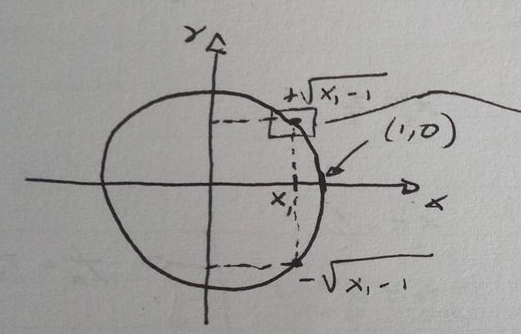
\includegraphics[width=0.5\textwidth]
			{images/f_impl1.png}
			\caption{\label{fig:my-label}}}
	\end{figure}
	
	Se però restringiamo il campo di studio nel seguente modo
	\begin{figure}[!htb]
		\center{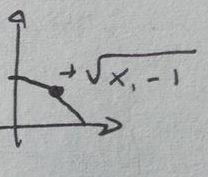
\includegraphics[width=0.3\textwidth]
			{images/f_impl2.png}
			\caption{\label{fig:my-label}}}
	\end{figure}
	
	Notiamo che abbiamo un grafico di funzione validissimo.
\end{enumerate}

Quello che traiamo da questi due esempi è che affinché sia definita una funzione implicta devono esserci condizioni molto stringenti, e sarà valido solo per ben definite regioni di piano. 

\bigskip

Ci viene in aiuto il teorema di Dini, nelle prossime pagine.

\newpage 
\subsection{Th. di Dini per funzioni scalari ad una variabile}

\textit{siano $\deffuncR{2}{}$ tale che}
\begin{enumerate}
	\item $f\in C^0(A)$
	\item $\exists f_y\in C^0(A)$
\end{enumerate}

\textit{e $(x_0,y_0)\in A$ tale che}

\begin{enumerate}
	\item $f(x_0,y_0)=0$
	\item $f_y(x_0,y_0)\neq0$
\end{enumerate}

\textit{Allora si ha che}
\begin{align}
	{}&\exists I(x_0),J(y_0) \taleche I \times J \in A\\ 
	&I \times J\taleche \exists ! y \in J \taleche f(x,y)=0
\end{align}

\textit{Possiamo quindi definire l'applicazione}
\begin{align}
	g=g(x) \taleche I \longrightarrow J \spacer g(x)\in C^0(I)
\end{align}

\textit{definita implicitamente da $f(x,g(x))=0$, con l'unicità di $y$ che impone $g(x_0)=y_0$.}

\bigskip

Il teorema può essere dimostrato in diversi modi. Quello che noi useremo si appoggia al \textbf{principio delle contrazioni}. La dimostrazione si snoda in tre passi, che vediamo dalla pagina successiva.

Come step preliminare riscriviamo la tesi in modo comodo
\begin{align}
	{}&f(x,y)=0 \leftrightarrow \frac{f(x,y)}{f_y(x_0,y_0)}=0 \leftrightarrow y-\frac{f(x,y)}{f_y(x_0,y_0)}=y\leftrightarrow G(x,y)=y\\
	&G(x_0,y_0)= y_0-\frac{f(x_0,y_0)}{f_y(x_0,y_0)}=y_0 - 0 = y_0\\
	&G_y(x,y)= 1- \frac{f_y(x,y)}{f_y(x_0,y_0)} \\
	&G_y(x_0,y_0)= 1 - \frac{f_y(x_0,y_0)}{f_y(x_0,y_0)} = 1 - 1=0
\end{align}

E definendo gli intorni come
\begin{align}
	{}&I(x_0)= (x_0 - r \spacecomma x_0 + r)\\
	&J(y_0)= (y_0 - \epsilon \spacecomma x_0 + \epsilon)\\
	&\overline{I} \times \overline{J}\in A
\end{align}

\begin{enumerate}
	\item \textbf{I passo:} Dimostrare che $(X,||\cdot||_\infty)$ è uno spazio metrico completo, dato $X= \{g\in C^0(I) \taleche ||g-y_=||_\infty <\epsilon\}$
	
	Ci basta trovare una successione di Cauchy $g_n$ tale che 
	\begin{align}
		\{g_n\} \in X \taleche g_n \longrightarrow \vecx \in X \subset C^0(\overline{I})
	\end{align}
	Siccome già sappiamo che 
	\begin{align}
		{}&\{g_n\} \text{ di Cauchy in } C^0(\overline{I}) \text{ completo}\\	
		&\exists g \in C^0(\overline{I}) \taleche g_n
		\overset{||\cdot||_\infty}{\longrightarrow} g
	\end{align}
	Ci basta dimostrare che $g\in X$. Siccome $g_n \in  X$ allora
	\begin{align}
		| g_n(x) - y_0| < || g_n(x) - y_0||_\infty \leq \epsilon \quad \forall x \in \overline{I}
	\end{align}
	
	Siccome $g_n \arrowlim{n}{\infty} g$ si ha che 
	\begin{align}
		\limit{n}{\infty}| g_n(x) - y_0| = | g(x) - y_0|\leq \epsilon \quad \forall x \in \overline{I}
	\end{align}
	
	Che implica a sua volta
	\begin{align}
		|| g(x) - y_0||_\infty\leq \epsilon \quad \forall x \in \overline{I} \implies g(x)\in X
	\end{align}
	
	e abbiamo finito il primo passo.
	
	\item \textbf{II passo:} Cerchiamo ora di dimostrare come $G(x,g(x))$ sia una contrazione. Ovvero definita
	\begin{align}
		T[g](x) = G(x,g(x)) \taleche X \longrightarrow C^0(\overline{I})
	\end{align}
	Innanzitutto ci serve che
	\begin{enumerate}
		\item $X= C^0(\overline{I})$
		\item $||T[g](x) - y_0||_\infty$
	\end{enumerate}
	Sia ora $x \in I$, avremo che
	\begin{align}
		|T[g] - y_0| {}&= |G(x,g(x)) - y_0| = |G(x,g(x)) - G(x_0,g(x_0))|= \continue
		&= |G(x,g(x)) - G(x_0,g(x_0))  + G(x,y_0) - G(x,y_0)|\leq \continue
		&\leq |G(x,g(x)) - G(x,y_0)| + |G(x,y_0) - G(x_0,g(x_0))|   
	\end{align}
	Studiamo separatamente i due pezzi:
	\begin{enumerate}
		\item Facendo uso di Lagrange 1D, e ponendoci in 
		\begin{align}
			\eta \in [y_0 \spacecomma g(x)]\subset [y_0 - \epsilon \spacecomma y_0 + \epsilon ]
		\end{align}
		Potremo scrivere
		\begin{align}
			|G(x,g(x)) - G(x,y_0)| {}&= |G(x,\eta) (g(x) - y_0)| \leq  \continue 
			&\leq \half |g(x) - y_0|  \leq \continue
			&\leq \half ||g(x) - y_0||_\infty \leq \half \epsilon
		\end{align}
		Questo perché, essendo $G_y(x_0,y_0)=0$, in un intorno di tale punto si ha che $G_y(x,y)$ è molto piccola e si può maggiorare con $\half$.
		
		\item Il secondo pezzo è più semplice, basta proseguire nel seguente modo:
		\begin{align}
			{}&|G(x,y_0) - G(x_0,g(x_0))| \leq \half \epsilon \quad \forall x \in I(x_0)\\ 
			&I(x_0)\subset [x_0 - r \spacecomma x_0 + r]
		\end{align}
	\end{enumerate}
	Da cui segue infine 
	\begin{align}
		|T[g] - y_0| \leq \half \epsilon + \half \epsilon = \epsilon \implies \underset{I}{max}|T[g] - y_0| \leq \epsilon \quad \forall x \in \overline{I}
	\end{align}
	Il che vuol dire che
	\begin{align}
		||T[g] - y_0||_\infty \leq  \epsilon \quad \forall x \in \overline{I}
	\end{align}
	Che è il risultato cercato.
	
	\item \textbf{III passo:} Dimostriamo l'altra condizione affinché $G(x,g(x))$ sia una contrazione, ovvero che
	\begin{align}
		\exists \alpha \in (0,1) \taleche ||T[g] - T[h]||_\infty \leq \alpha || g -h  ||_\infty 
	\end{align}
	Avremo che
	\begin{align}
		||T[g] - T[h]||_\infty = ||G(x,g(x)) - G(x,h(x))||_\infty
	\end{align}
	Usando di nuovo il th. di Lagrange nello stesso modo del punto precedente avremo
	\begin{align}
		||T[g] - T[h]||_\infty = ||G_y(x,\eta) (g(x) -h(x))||_\infty
	\end{align}
	Analogamente a prima, dato che  $G(x_0,y_0)=0= G_y(x_0,y_0)$ avremo che per $\forall \eta \in [h(x)\spacecomma g(x)]\subset[y_0 - \epsilon \spacecomma y_0 + \epsilon]$
	Sicuramente avremo
	\begin{align}
		|G_y(x,\eta)|\leq \half
	\end{align}
	Ma essendo $\half \in (0,1)$ lo possiamo assumere come valore di $\alpha$! Ci troviamo quindi ad avere
	\begin{align}
		||G(x,g(x)) - G(x,h(x))||_\infty = \half||g(x) - h(x)||_\infty
	\end{align}
	E abbiamo così dimostrato come $G(x,g(x))$ sia una contrazione! Possiamo quindi chiudere la dimostrazione applicando il \textbf{Principio di contrazione}:
	\begin{align}
		\exists ! g \in X \taleche T[g](x)) = g(x)\\
		\updownarrow \continue 
		G(x,g(x))=g(x) \\
		\updownarrow \continue
		f(x,g(x))=0
	\end{align}
\end{enumerate}


Il th. di Dini ci garantisce l'esistenza, ma non  ci dice che forma abbia $g(x)$. 

Ci serve quindi di enunciare il seguente \textbf{teorema}:

\bigskip

\textit{Se valgono le ipotesi del teorema di Dini, con aggiunta la condizione}
\begin{align}
	\exists f_x(x,y)\in C^0(A)\implies f(x,y)\in C^1(A)
\end{align}
\textit{Allora possiamo scrivere}
\begin{align}
	g'(x)= - \frac{f_x(x,y)}{f_y(x,y)}
\end{align}
\textit{E se $f\in C^k(I)$ allora avremo che}
\begin{align}
	g^{(k)}(x) = \dertotk{k-1}{}{x} g'(x)= - \dertotk{k-1}{}{x} \left( \frac{f_x(x,y)}{f_y(x,y)} \right)
\end{align}

\bigskip

Per la dimostrazione iniziamo ponendo
\begin{align}
	{}&f(x,g(x))= 0 \implies f(x+h,g(x+h))=0 \quad \forall x \spacecomma x+h \in I(x_0) \nextpassage
	&f(x+h,g(x+h)) - f(x,g(x)) = 0
\end{align}
Il th. di Lagrange in due variabili afferma che
\begin{align}
	f(x_1,y_1) - f(x_2,y_2) = f_x(x_3,y_3)(x_1-x_2) + f_y(x_3,y_3)(y_1 - y_2) 
\end{align}
Da cui otteniamo, posto $(\xi,\eta)\in [(x+h,g(x+h)) \spacecomma (x,g(x))]$
\begin{align}
	{}&0=f(x+h,g(x+h)) - f(x,g(x)) = f_x(\xi,\eta)h+ f_y(\xi,\eta) (g(x+h) - g(x)) \nextpassage
	&f_x(\xi,\eta)h=  - f_y(\xi,\eta) (g(x+h) - g(x)) \nextpassage
	&\frac{g(x+h) - g(x)}{h} = - \frac{f_x(\xi,\eta)}{f_y(\xi,\eta)} \nextpassage
	&\limit{h}{0} \frac{g(x+h) - g(x)}{h} = - \limit{h}{0} \frac{f_x(\xi,\eta)}{f_y(\xi,\eta)}
\end{align}
Siccome per $h\rightarrow 0$ si ha che
\begin{align}
	{}&(\xi,\eta)\in [(x+h,g(x+h)) \spacecomma (x,g(x))] \arrowlim{h}{0} [(x,g(x)) \spacecomma (x,g(x))] \nextpassage
	&(\xi,\eta) = (x,g(x))
\end{align}
Allora si ottiene il risultato cercato
\begin{align}
	{}&g'(x)=\limit{h}{0} \frac{g(x+h) - g(x)}{h} = - \limit{h}{0} \frac{f_x(\xi,\eta)}{f_y(\xi,\eta)} = - \frac{f_x(x,y)}{f_y(x,y)} \nextpassage
	&g'(x)= - \frac{f_x(x,y)}{f_y(x,y)}
\end{align}

Una dimostrazione più semplice ma che può essere applicata solo per funzioni di classe $C^1$ si basa sulla formula delle derivate di funzioni composte che già conosciamo.

\bigskip

\textbf{Nota bene:} Tutti i risultati ricavati finora possono essere ricavati a variabili invertite, basta scambiare le condizioni.

\bigskip

Chiudiamo il discorso mostrando l'espresione delle derivate al II ordine:
\begin{align}
	{}&f \in C^2(A) \implies g\in C^2(A)\\
	&g'(x) = - \frac{f_x(x,y)}{f_y(x,y)} \nextpassage
	&g'(x)f_y(x,y) = -f_x(x,y) \nextpassage
	& g'(x)f_y(x,y) + f_x(x,y)=0 \nextpassage
	&\dertot{}{x} (g'(x)f_y(x,y) + f_x(x,y))=0 \nextpassage
	&f_{xx}(x,y) + f_{xy}(x,y)g'(x) + [f_{xy}(x,y) + f_{yy}(x,y)g'(x)]\cdot g'(x) + f_y(x,y)g''(x)=0 \nextpassage
	& f_{xx}(x,y) + 2f_{xy}(x,y)g'(x) + f_{yy}(x,y)[g'(x)]^2 + f_y(x,y)g''(x)=0\nextpassage
	&g''(x) = -\frac{f_{xx}(x,y) + 2f_{xy}(x,y)g'(x) + f_{yy}(x,y)[g'(x)]^2}{f_y(x,y)}
\end{align}

Se $g'(x)=0$ l'espressione si semplifica notevolmente in $g''(x) = -\frac{f_{xx}(x,y)}{f_y(x,y)}$

\subsection{Esempi di esercizi}

\begin{enumerate}
	\item Data l'equazione
	\begin{align}
		x \Exp{y}=y
	\end{align}
	
	\begin{enumerate}
		\item Dire se in un intorno di $(0,0)$ essa descrive una curva $(x,g(x))$
		\item Determinare l'equazione della retta tangente alla curva in $x=0$
		\item Tracciare un grafico approssimativo
	\end{enumerate}
	
	\bigskip
	Procediamo in ordine:
	\bigskip
	
	\begin{enumerate}
		\item Verifichiamo se la nostra $f(x,y)= x \Exp{y}-y$ rispetta le condizioni di Dini:
		\begin{align}
			{}& f \in C^k(\R^2) \quad \forall k\\ 
			&f(0,0)= 0\\
			&f_y(x,y)= x \Exp{y}-1 \implies f_y(0,0)= 0-1 = -1 \neq 0 \\
			&f_x(x,y)= \Exp{y} \implies f_x(0,0)= 1
		\end{align}
		Le condizioni sono rispettate, quindi avremo
		\begin{align}
			{}&\exists I(x_0)\times J(y_0) \subset A \taleche \forall x\in I(x_0) \quad \exists ! y \in J(y_0) \taleche x\Exp{y}-y=0\\
			& y = y(x) \taleche I \longrightarrow J \spacer g(0)=0 \spacer g^k(I)
		\end{align}
		
		\item La retta tangente è data da\begin{align}
			{}&y= y_0 + g'(x_0)(x-x_0)= 0 - \left. \frac{f_x}{f_y}\right|_{(0,0)}x= 0 - \frac{1}{-1}x=x\nextpassage
			&y -x =0
		\end{align} 
		
		\item Per tracciare il grafico della funzione abbiamo bisogno delle derivate successive
		\begin{align}
			{}&f_{xx} = 0 \implies f_{xx}(0,0) = 0\\
			&f_{xy} = \Exp{y}=f_{yx} \implies f_{xy}(0,0) = 1\\
			&f_{yy}= x\Exp{y}\implies f_{yy}(0,0) = 0\\
			&g''(0)= -\frac{0 +2 + 0}{-1}=2
		\end{align}
		
		E con Taylor avremo
		\begin{align}
			g(x)= g(0) + g'(0)x + \half g''(0)x^2 + o(x^2)= 0+x+x^2 + o(x^2)
		\end{align}	
	\end{enumerate}
		
	\item Data l'equazione
	\begin{align}
		e^x \sin(y) + e^y\cos(x)-1=0
	\end{align}
	In un intorno di $(0,0)$
	\begin{enumerate}
		\item Verificare l'esistenza di una funzione implicita 
		\item Verificare che in $x=0$ abbia un punto critico
		\item Categorizzare tale punto
	\end{enumerate}
	
	\bigskip
	\begin{enumerate}
		\item Verifichiamo le condizioni di Dini
		\begin{align}
			{}&f\in C^k(I)\\
			& f(0,0)=1-1=0\\
			& f_y= e^x \cos(y) + e^y\cos(x) \implies f_y(0,0)= 1+1=2\neq 0 \\
			& f_x= e^x \sin(y) - e^y\sin(x) \implies f_y(0,0)= 1\cdot 0+0\cdot 1= 0
		\end{align}
		
		Le condizioni sono verificate, e abbiamo quindi sicuro una $g(x)$
		
		\item Verificare che in $x=0$ abbia un punto critico
		\begin{align}
			g'(0)=-\frac{f_x(0,0)}{f_y(0,0)}=-\frac{0}{2}=0
		\end{align}
		Quindi $x=0$ è punto critico
		
		\item Categorizziamo tale punto
		\begin{align}
			f_{xx}= e^x \sin(y) - e^y\cos(x) \implies f_{xx}(0,0)= -1
		\end{align}
		Siccome $g'(0)=0$ possiamo usare la forma ridotta
		\begin{align}
			g''(0)= -\frac{f_{xx}(0,0)}{f_y(0,0)}= - \frac{-1}{2}= \half > 0 
		\end{align}
		E quindi $x=0$ è un punto di minimo. 
	\end{enumerate}
	
	\item Data l'equazione
	\begin{align}
		y^2 + x+ \Exp{x^2 + y^2} -1 =0
	\end{align}
	
	Studiamo le stesse richieste del precedente esercizio in un intorno di $(0,0)$, con aggiunto il calcolo della retta tangente.
	
	\begin{enumerate}
		\item Verifichiamo le condizioni di Dini
		\begin{align}
			{}&f\in C^k(I)\\
			& f(0,0)=0+0+ 1-1=0\\
			& f_y= 2y(1+\Exp{x^2 + y^2})\implies f_y(0,0)= 0 \\
			& f_x= 1 + 2\Exp{x^2 + y^2} \implies f_x(0,0)= 1+0=1\neq 0
		\end{align}
		Ci troviamo stavolta nel caso opposto, che avevamo brevemente detto esistere. Avremo cioè che
		\begin{align}
			\exists I(x_0)\times J(y_0) \taleche \forall y \in J \quad \exists ! x \taleche f(h(y),y)=0
		\end{align} 
		
		\item Avremo in $y=0$ un punto critico, infatti
		\begin{align}
			h'(0)= -\frac{f_y(0,0)}{f_x(0,0)} =0
		\end{align}
		
		\item Per classificare $y=0$ ci basta calcolare
		\begin{align}
			{}&f_{yy}(0,0)= [2(1+\Exp{x^2 + y^2}) - 4y^2\Exp{x^2 + y^2}]|_{(0,0)}= 4\\&h''(0)=-\frac{f_{yy}(0,0)}{f_x(0,0)}=-4
		\end{align}
		Abbiamo quindi un punto di massimo
		
		\item La retta tangente avrà equazione
		\begin{align}
			h(y)= h(0) + h'(0)y + \half h''(0)y^2 + o(y^2)= 2y^2 + o(y^2)
		\end{align}
	\end{enumerate}
\end{enumerate}

\newpage

\subsection{Teorema di Dini per funzioni scalari a più variabili}
\textit{Siano}
\begin{align}
	{}&\vecx= (x_1,\dots, x_n)\in \R^n\spacer y \in \R\\
	&f(\vecx,y) \taleche A \subseteq \R^{n+1} \longrightarrow \R
\end{align}
\textit{Se valgono le seguenti condizioni in $(\vecx^0,y_0)\in A$}
\begin{enumerate}
	\item $f(\vecx,y)\spacecomma f_y(\vecx,y)\in C^0(A)$
	\item $(\vecx^0,y_0) \taleche f(\vecx^0,y_0) =0 \neq f_y(\vecx^0,y_0)$ 
\end{enumerate}
\textit{Allora si ha che}
\begin{align}
	{}&\exists I(\vecx^0) = \{\vecx \taleche |\vecx - \vecx^0|\leq r \} \text{ intorno sferico}\\
	&\exists J(y_0)=(y_0-\epsilon \spacecomma y_0+\epsilon)
\end{align}
\textit{con}
\begin{align}
	I \times J \subset A \taleche \forall \vecx \in I \quad \exists ! y \taleche f(x,y)=0 \leftrightarrow y= g(\vecx) \taleche I\longrightarrow J
\end{align}
\textit{Inoltre se $f\in C^1(A)$ si ha che anche $g\in C^1(I)$ e si può scrivere}
\begin{align}
	g_{x_i}= - \frac{f_{x_i} (\vecx,g(\vecx))}{f_y(\vecx,g(\vecx))}
\end{align}

\bigskip
Non diamo la dimostrazione del teorema, non essendoci necessaria ai fini del corso. Ci chiediamo però: in termini pratici, che ci dice questa versione del teorema? Notiamo come in realtà sia una forma più generale del caso che abbiamo già enunciato, che è qui rappresentato nel caso $n=1$, mentre il caso $n=2$ sarà
\begin{align}
	{}&\deffuncR{3}{}\\
	&\Sigma = \{\vecP = (x,y,z) \taleche f(\vecP)=0 \}\\
	& \vecP^0\in A \taleche f(\vecP^0)=0\neq f_z(\vecP^0)\\
	&z= g(x,y) \\
	&g_x = - \left. \frac{f_x}{f_z}\right|_{\vecP^0} \spacer g_y = - \left. \frac{f_y}{f_z}\right|_{\vecP^0}\\
	&T(z,\vecP^0)= z_0 + g_x(x_0,y_0) (x-x_0) + g_y(x_0,y_0)(y-y_0)
\end{align}

Vediamo, per chiarirci di più le idee, un \textbf{esempio:}
\begin{align}
	{}&\Exp{z} + z\Exp{x+y} - \Exp{x-y}=0 \implies f(x,y,z)= \Exp{z} + z\Exp{x+y} - \Exp{x-y}\\
	& f\in C^k(\R^3) \quad \forall k\\
	& f_z(x,y,z)= \Exp{z} + \Exp{x+y} \implies f_z(0,0,0)= 1+1 = 2 \neq 0
\end{align}

Avremo quindi
\begin{align}
	g(x,y)	\in C^k(I) \quad \forall k \taleche I(0,0) \subset \R^2 \longrightarrow J(0,0) \subset \R 
\end{align}

Andiamo a calcolarne il piano tangente:
\begin{align}
	{}&f_x= z\Exp{x+y} - \Exp{x-y} \implies f_x(0,0) = -1 \\
	&f_y = z\Exp{x+y} + \Exp{x-y}\implies f_y(0,0) = +1 \\
	&T(z,\vecP^0) = 0 - \left(\half\right)x - \left(\half\right)y= \half (x-y)
\end{align}

\newpage 

\subsection{Teorema di Dini per sistemi di funzioni}

Poniamoci ora la seguente domanda: chi chiediamo se il sistema
\begin{align}
	\double{f(x,y,z)=0}{g(x,y,z)=0}
\end{align}
Possa definire una curva $\gamma$ tale che
\begin{align}
	\underline{r}(t)=\triple{x=t}{y=y(t)}{z=z(t)}
\end{align}

La risposta è: dipende.

Ad esempio col seguente sistema
\begin{align}
	\double{ax + by + cz + d=0}{\alpha x + \beta y + \gamma z  + \delta=0} \implies \double{ by + cz =- d -ax}{\beta y + \gamma z =  - \delta - \alpha x}
\end{align}

Avremo una soluzione solo se è rispettata la \textbf{condizione di Kramer}, ovvero
\begin{align}
	\det \matrixTwoTwo{b}{c}{\beta}{\gamma} \neq 0
\end{align}

Affinché quindi abbia soluzione il sistema e si possa definire la curva che rappresenta l'intersezione tra i due piani servono condizioni restrittve. 

Enunciamo il \textbf{Teorema di Dini per sistemi di funzioni:}

\bigskip

\textit{Se si ha}
\begin{align}
	{}&f(x,y,z),g(x,y,z) \in C^1(A) \spacecomma A\subset \R^3\\
	&\vecP^0=(x_0,y_0z_0) \taleche f(\vecP^0)=0=g(\vecP^0) \spacer \det \left. \matrixTwoTwo{f_y}{f_z}{g_y}{g_z}\right|_{\vecP^0}\neq 0
\end{align}
\textit{Allora avremo che}
\begin{align}
	{}&\exists I(x_0) = (x_0 - r \spacecomma x_0 +r) \spacecomma J(x_0,y_0)\subset \R^2\\
	&I \times J \subset A \taleche \exists ! (y,z)\in J \text{ soluzioni del sistema } \double{f(x,y,z)=0}{g(x,y,z)=0} \taleche \double{y=y(x)}{z=z(x)} \text{ per } x\in I
\end{align}

Che forma avranno le derivate? Proviamo a calcolarle
\begin{align}
	{}&\double{f(x,y,z)=0}{g(x,y,z)=0} \implies \double{f_x + f_y y' + f_z z'=0}{g_x + g_y y' + g_z z'=0} \nextpassage 
	&\double{f_x +  f_z z' = -f_y y' }{g_x + g_z z'=-g_y y'} \spacer \double{f_y y' +  f_z z'= -f_x }{g_y y'+ g_z z'=-g_x}
\end{align}

Come nell'esempio prima avremo che devono valere
\begin{align}
	\det \matrixTwoTwo{-f_x}{f_z}{-g_x}{g_z} \neq 0 \spacer \det \matrixTwoTwo{f_y}{-f_x}{g_y}{-g_x} \neq 0
\end{align}
Da cui ricaviamo
\begin{align}
	y'(x)= - \left. \frac{\matrixTwoTwo{-f_x}{f_z}{-g_x}{g_z}}{\det  \matrixTwoTwo{f_y}{f_z}{g_y}{g_z}} \right|_{(x,y)}
	\spacer
	z'(x)= - \left. \frac{\matrixTwoTwo{f_y}{-f_x}{g_y}{-g_x}}{\det  \matrixTwoTwo{f_y}{f_z}{g_y}{g_z}} \right|_{(x,y)}
\end{align}

\newpage 

\subsection{Teorema di Dini nel caso generale}

\textit{Siano}
\begin{align}
	\vecf \taleche A \R^{n+m} {}&\longrightarrow \R^m\\
	(\vecx,\vecy) &\longrightarrow \vecf(\vecx,\vecy)= (f_1,\dots,f_m)|_{(\vecx,\vecy)} \continue
	\vecx=(x_1,\dots,x_n) &\spacer \vecy=(y_1,\dots , y_m)
\end{align}
\textit{Se dato $(\vecx^0,\vecy^0)$ sono rispettate le seguenti proprietà}
\begin{align}
	{}&\vecf \in C^1(A)\\
	&(\vecx^0,\vecy^0) \taleche 	\vecf(\vecx^0,\vecy^0)=0\\
	&\det \left.\left(\partialder{\vecf}{\vecy}\right)\right|_{\vecP^0} \neq 0 \spacer \left(\partialder{\vecf}{\vecy}\right) = \left(\partialder{f_i}{y_j}\right)_{\scriptsize{\begin{array}{cc}
				i=1,\dots,m\\
				j=1,\dots,n
	\end{array}}}
\end{align}
\textit{Allora si ha che esistono}
\begin{align}
	\exists I(\vecx^0) \subset \R^n \spacecomma J(\vecy^0)\subset \R^m \taleche I\times J \subset \R^{n+m}
\end{align}
\textit{Tali che}
\begin{align}
	{}&\forall \vecx\in I \quad\exists ! \vecy \taleche \vecf(\vecx,\vecy) =\veczero\\
	&\vecy = \vecg(\vecx)\in C^1(I)\taleche I\subset \R^n \longrightarrow J \subset \R^m \\
	&\jacobian \vecg(\vecx)= -  \left(\partialder{\vecf}{\vecy}\right)^{-1} \left(\partialder{\vecf}{\vecx}\right)
\end{align}

\subsection{Invertibilità Locale}

Un'interessante applicazione del teorema di Dini si ha nello studio dell'invertibilità locale delle funzioni.

Supponiamo di avere
\begin{align}
	\vecf \taleche A \subset \R^n \longrightarrow B \subset \R^n
\end{align}
Con $A,B$ aperti e $\vecf(\vecx)\in C^1(A)$.

Ci chiediamo: sotto quali ipotesi $\vecf$ è invertibile localmente in $A$, con $\vecf^{-1}\in C^1(B)$? O, in altri termini, quando $\vecf$ è un \textbf{diffeomorfismo} locale tra $A$ e $B$? 

Ci viene in aiuto il \textbf{Teorema di Inversione Locale:}

\bigskip

\textit{Siano}
\begin{align}
	{}&\vecf \taleche A \subset \R^n \longrightarrow B \subset \R^n\\
	&f\in C^1(A)\\
	&\vecx^0 \in A
\end{align}
\textit{Se}
\begin{align}
	\det \jacobian{\vecf}{\vecx^0} = \det\left( \partialder{f_i}{x_j} \right)_{\scriptsize{
			\begin{array}{cc}
				i=1,\dots,n\\
				j=1,\dots n
			\end{array}
	}} \neq 0
\end{align}
\textit{Allora f è localmente invertibile.}

\bigskip

La dimostrazione discende dal caso generale di Dini. 

Posti
\begin{align}
	{}&\vecF (\vecx,\vecy)= \vecy - \vecf(\vecx)\\
	& \vecy^0 = \vecf(\vecx^0)
\end{align}
Applichiamo Dini in $(\vecx^0,\vecy^0)$. Le ipotesi sono verificate per costruzione, dato che
\begin{align}
	{}&\vecF (\vecx^0,\vecy^0)= \vecy^0 - \vecf(\vecx^0) = \vecy^0 - \vecy^0 =0\\
	&\vecF\in C^1(A \times \R^n)\\
	& \left. \partialder{\vecF}{\vecx} \right|_{(\vecx^0,\vecy^0)} = - \left. \partialder{\vecf}{\vecx} \right|_{(\vecx^0,\vecy^0)} \neq 0 \text{ per ipotesi}
\end{align}
Questo vuol dire che
\begin{align}
	\exists I(\vecx^0),J(\vecy^0) \taleche \forall \vecy \in J \quad \exists \vecx = \vech(\vecy) \in I \taleche \vecF (\vech(\vecy),\vecy) =0
\end{align}
Ma questo vuol dire anche che
\begin{align}
	\vecy = \vecf(\vech(\vecy)) \implies \vech(\vecy)= \vecf^{-1}(\vecy)
\end{align}
E il teorema è dimostrato.

\bigskip

Le derivate avranno forma
\begin{align}
	\partialder{\vech(\vecy)}{\vecy} = -\left( \partialder{\vecF}{\vecx} \right)^{-1}\left( \partialder{\vecF}{\vecy} \right)
\end{align}
Ma per come abbiamo definito $\vecF$ il secondo termine diventa
\begin{align}
	\partialder{\vech(\vecy)}{\vecy} = -\left( \partialder{\vecF}{\vecx} \right)^{-1} \mathbb{1}_n = -\left( \partialder{\vecF}{\vecx} \right)^{-1} \implies \jacobian{f^{-1}}{\vecx}= (\jacobian{f}{\vecx})^-1
\end{align}
Ma a noi tutto questo è familiare! Infatti in $\R$ avevamo che se
\begin{align}
	y=f(x)\in C^1((a,b)) \spacer f'(x_0)\neq 0 \spacecomma x_0\in (a,b)
\end{align}
Allora 
\begin{align}
	\dertot{}{y}f^{-1}(y)= \fracn{f'(f^{-1}(y))}
\end{align}
La differenza giace però nell'invertibilità globale. Infatti mentre in $\R$ la derivabilità in tutto l'insieme implica monotonia e quindi invertibilità in tutto l'insieme, in $\R^{n>1}$ non è detto, come vediamo nel seguente \textbf{esempio in $\R^2$:}
\begin{align}
	{}&\vecy = \vecf(\vecx)= \double{y_1= \Exp{x_1} \cos(x_2)}{y_2= \Exp{x_1} \sin(x_2)}\\
	\continue
	& \jacobian{\vecf}{\vecx}=\partialder{\vecf}{\vecx}= \matrixTwoTwo{f_{1_{x_1}}}{f_{1_{x_2}}}{f_{2_{x_1}}}{f_{2_{x_2}}} = \matrixTwoTwo{+\Exp{x_1} \cos(x_2)}{-\Exp{x_1} \sin(x_2)}{+\Exp{x_1} \sin(x_2)}{+\Exp{x_1} \cos(x_2)}
\end{align}
Da cui segue che 
\begin{align}
	\det \jacobian{\vecf}{\vecx}= \Exp{2x}\neq 0 \quad \forall \vecx
\end{align}
Però la funzione non è iniettiva, e quindi non può essere invertibile globalmente. 

\section{Punti di massimo e minimo vincolati}

Per amor di semplicità studiamo il problema nel piano.

Dati
\begin{align}
	{}&\deffuncR{2}{}\\
	&\deffuncRgen{g}{2}{}\\
	&Z= \{ (x,y)\in A \taleche g(x,y)=0 \}\neq \emptyset
\end{align}
Definiamo $(x_0,y_0)$ 
\begin{enumerate}
	\item \textbf{punto di max. vincolato di $f$ su Z} se
	\begin{align}
		f(x,y)\leq f(x_0,y_0) \quad \forall (x,y)\in Z \cap I(x_0,y_0)
	\end{align}
	\item \textbf{punto di min. vincolato di $f$ su Z} se
	\begin{align}
		f(x,y)\geq f(x_0,y_0) \quad \forall (x,y)\in Z \cap I(x_0,y_0)
	\end{align}
\end{enumerate}

Ci domandiamo: perché stiamo studiando di nuovo il problema? Non abbiamo già il teorema di Fermat? La risposta è \textbf{no}, visto che Fermat considera \underline{solo} gli insiemi aperti!

\bigskip

Siamo quindi costretti a trovare altre vie per tale studio. 

\bigskip

Un metodo lo conosciamo già, dato che $Z$ è una curva: parametrizziamo nel seguente modo
\begin{align}
	Z=\{ (x(t),y(t)) \spacecomma t \in [a,b] \}
\end{align}
E ci troviamo a studiare una funzione in $\R$, dove abbiamo tutti gli strumenti per lavorare:
\begin{align}
	f(x,y)|_Z = f(x(t),y(t)) =F(t)
\end{align}

\bigskip

Un altro metodo molto interessante è quello dei \textbf{Moltiplicatori di Lagrange}, che vediamo nella pagina successiva.

\newpage

\subsection{Metodo dei Moltiplicatori di Lagrange in $\R^2$}

\textit{Se abbiamo}
\begin{enumerate}
	\item $f,g \in C^1(A)$
	\item $(x_0,y_0)\in A$ tale che
	\begin{enumerate}
		\item $g(x_0,y_0)=0 \leftrightarrow (x_0,y_0)\in Z$
		\item $\gradient{g}{x_0,y_0}\neq 0 \leftrightarrow (x_0,y_0)$ punto regolare
		\item $(x_0,y_0)$ punto di max. (o min.) vincolato per $f$
	\end{enumerate}
\end{enumerate}

\textit{Allora avremo un risultato che può essere enunciato in tre modi equivalenti:}
\begin{enumerate}
	\item $\left. \det \matrixTwoTwo{f_x}{f_y}{g_x}{g_y}\right|_{(x_0,y_0)} = 0$
	\item $\exists \lambda_0 \in \R \taleche \gradient{f}{x_0,y_0}= \lambda_0 \gradient{f}{x_0,y_0}$
	\item \textit{Data }$L(x,y,\lambda)= f(x,y) - \lambda g(x,y)$ $\exists \lambda_0 \taleche \gradient{L}{x_0,y_0, \lambda_0}=\veczero$ 
\end{enumerate}

Prima di dare la dimostrazione mostriamo perché le tre formulazioni siano equivalenti:

La prima scrittura implica che i gradienti siano \textbf{linearmente dipendeti} e che quindi $\exists \lambda_0 \taleche \gradient{f}{x_0,y_0}= \lambda_0 \gradient{f}{x_0,y_0}$ che è la seconda scrittura.

La terza implica che
\begin{align}
	\triple{L_x(x_0,y_0, \lambda_0) = {}&[f_x - \lambda_0 g_x]|_{(x_0,y_0, \lambda_0)}=0}{L_y(x_0,y_0, \lambda_0) = &[f_y - \lambda_0 g_y]|_{(x_0,y_0, \lambda_0)}=0}{L_\lambda(x_0,y_0, \lambda_0) = &-g|_{(x_0,y_0, \lambda_0)}=0}
\end{align}
La terza derivata è un'ipotesi, le altre due altro non sono che il secondo enunciato.

Vediamo come dimostrare il teorema.

Per ipotesi in $(x_0,y_0)$ abbiamo che
\begin{align}
	g_y(x_0,y_0) \neq 0 = g(x_0,y_0)
\end{align}
Possiamo quindi applicare il teorema di Dini, da cui abbiamo che
\begin{align}
	\exists I(x_0)\times J(y_0) \taleche \forall x \quad \exists ! y=h(x) \taleche f(x,h(x))=0
\end{align}
Sia ora $\vecP^0=(x_0,y_0)$ punto di max.vincolato, ovvero
\begin{align}
	{}&f(x,y)\leq f(x_0,y_0) \quad \forall (x,y)\in Z\cap  I(x_0)\times J(y_0) \nextpassage
	& f(x,h(x)) \leq f(x_0,h(x_0)) \quad \forall x\in I(x_0) \nextpassage
	& F(x)\leq F(x_0)  \quad \forall x\in I(x_0)= (x_0 - r \spacecomma x_0 + r)
\end{align}
Per Fermat avremo che
\begin{align}
	{}&F'(x_0)=0 \nextpassage
	&\dertot{}{x}f(x_0,h(x_0))=0\nextpassage						&f_x(x_0,h(x_0)) + f_y(x_0,h(x_0))h'(x_0)=0\nextpassage
	&f_x(x_0,h(x_0)) - f_y(x_0,h(x_0))\frac{g_x(x_0)}{g_y(x_0)}=0  \quad\text{per il th. di Dini} \nextpassage
	& \frac{f_x(x_0,h(x_0))g_y(x_0) - f_y(x_0,h(x_0))g_x(x_0)}{g_y(x_0)}=0 \nextpassage
	&\fracn{g_y(x_0)} \det \left.\matrixTwoTwo{f_x}{f_y}{g_x}{g_y}\right|_{\vecP^0}=0 \nextpassage
	& \left.\det\matrixTwoTwo{f_x}{f_y}{g_x}{g_y}\right|_{\vecP^0}=0
\end{align}
Che è la nostra prima formulazione, e quindi il th. è dimostrato.

\newpage

Vediamo ora un \textbf{esempio:} la massimizzazione dell'area di rettangoli inscritti in un'ellisse.

\bigskip

Sia l'ellisse di equazione
\begin{align}
	\frac{x^2}{a^2} + \frac{y^2}{b^2}=1 \spacer a,b>0
\end{align}

E sia il rettangolo inscritto
\begin{align}
	f(x,y)= xy
\end{align}

Ci chiediamo
\begin{align}
	\underset{g(x,y)=0}{max}f(x,y)=?
\end{align}

Per quanto riguarda $f(x,y)$ sappiamo che
\begin{enumerate}
	\item $f(x,y)$ è continua su tutto $\R^2$
	\item $f(a,0)=f(0,b)=0$ 
\end{enumerate}

Ponendo ora
\begin{align}
	g(x,y)= \frac{x^2}{a^2} + \frac{y^2}{b^2}-1
\end{align}

E tenendo conto del fatto che la lunghezza dei lati del rettangolo deve essere positiva, avremo
\begin{align}
	Z=\{ (x,y) \taleche g(x,y)=0 \spacer x,y \geq 0 \} \subset [-a\spacecomma +a]\times [-b \spacecomma +b]
\end{align}

\begin{figure}[!htb]
	\center{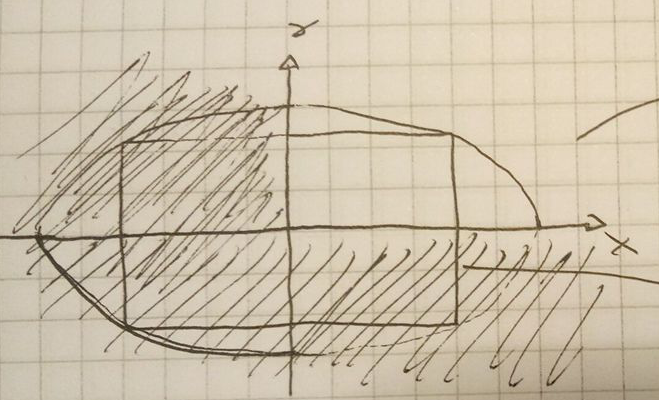
\includegraphics[width=0.5\textwidth]
		{images/esempio.png}
		\caption{\label{fig:my-label}}}
\end{figure}

$Z$ è chiuso e limitato e per Weierstrass sicuro esistono max. e min. su $Z$. 
Il minimo lo sappiamo già ad occhio, visto che abbiamo solo valori non negativi di $x$ e $y$ deve essere che
\begin{align}
	\underset{(x,y)\in Z}{min}f(x,y)=0 \implies (0,b) \spacecomma (a,0) \text{ punti di minimo}
\end{align}
Andiamo a trovare il massimo tramite Lagrange, ma prima accertiamoci che non ci siano punti non regolari:
\begin{align}
	{}&\gradient{g}{x,y}= \veccolTwo{\frac{2x}{a^2}}{\frac{2y}{b^2}} = \veccolTwo{0}{0} \implies (x,y)=(0,0)\\
	&\gradient{f}{x,y}=\veccolTwo{y}{x}=  \veccolTwo{0}{0} \implies (x,y)=(0,0)
\end{align}

Ma l'origine non è compresa in $Z$, quindi nessun problema.

Possiamo quindi applicare Lagrange, costruendo il sistema
\begin{align}
	\double{\det \matrixTwoTwo{y}{x}{\frac{2x}{a^2}}{\frac{2y}{b^2}}=0}{\frac{x^2}{a^2} + \frac{y^2}{b^2}=1}\implies
	\double{\frac{y^2}{b^2} - \frac{x^2}{a^2}=0}{\frac{x^2}{a^2} + \frac{y^2}{b^2}=1}
\end{align}

Da cui si ricava
\begin{align}
	\double{y^2 = \frac{b^2}{a^2}x^2}{\frac{2}{a^2}x^2=1} \implies x = \pm \frac{a}{\sqrt{2}} \spacer y= \pm \frac{b}{\sqrt{2}}
\end{align}

Scartando i risultati negativi per costruzione abbiamo trovato il nostro punto di massimo in
\begin{align}
	(x,y)_M= \left(\frac{a}{\sqrt{2}} \spacecomma \frac{b}{\sqrt{2}}\right)
\end{align}

\subsection{Esempi}

\begin{enumerate}
	\item Massimizzazione dell'area di rettangoli a somma dei lati costante.
	
	\bigskip
	
	Come prima avremo la funzione che descrive il perimetro
	\begin{align}
		f(x,y)=xy \spacer \gradient{f}{x,y}= (y \spacecomma x)
	\end{align}
	Mentre stavolta il vincolo sarà dato dall'equazione
	\begin{align}
		{}&x+y=c>0 \implies g(x,y)= x+y-c\\
		& Z=\{ x,y \geq 0 \taleche x+y=c \}
	\end{align}
	
	\begin{figure}[!htb]
		\center{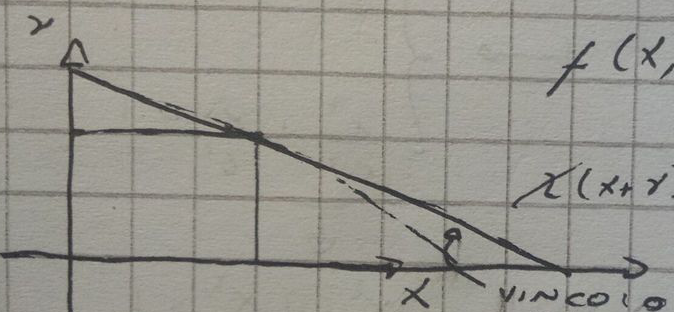
\includegraphics[width=0.5\textwidth]
			{images/esempio2.png}
			\caption{\label{fig:my-label}}}
	\end{figure}	
	
	$Z$ è chiuso e limitato, ergo per Weierstrass ci sono max. e min.
	
	Come nell'esempio precedente il minimo si avrà lungo gli assi, mentre per il massimo utlizziamo Lagrange:
	\begin{align}
		\double{\left.\det\matrixTwoTwo{f_x}{f_y}{g_x}{g_y}\right|_{\vecP^0}=0}{x+y=c} \implies
		\double{x-y=0}{x+y=c}
	\end{align}
	E otteniamo quindi un punto di massimo in
	\begin{align}
		(x,y)_M= \left( \frac{c}{2} \spacecomma \frac{c}{2} \right)
	\end{align}
	
	\bigskip
	
	\item Studiare l'esistenza di punti critici della funzione
	\begin{align}
		{}&f(x,y)= (x+1)^2 + (y-1)^2 \\ 
		&\gradient{f}{x,y} = (2(x+1) \spacecomma 2(y-1))
	\end{align}
	Con vincolo dato da
	\begin{align}
		{}&x^2 + y^2 = 4 \implies g(x,y)=x^2 + y^2 - 4
	\end{align}	
	Nel dominio chiuso e limitato
	\begin{align}
		D = \{ (x,y) \taleche g(x,y)\leq 0 \}
	\end{align}
	
	Siccome
	\begin{align}
		f\in C^0(\R^2) \implies f\in C^0(Z)
	\end{align}
	Quindi per Weierstrass abbiamo punti di massimo e minimo. Dividiamo lo studio in due parti:
	\begin{enumerate}
		\item \underline{punti interni:}
		Non esistono punti di non derivabilità, quindi cerchiamo solo punti critici:
		\begin{align}
			\gradient{f}{x,y} = \veczero \implies \veccolTwo{2(x+1)}{2(y-1)} = \veccolTwo{0}{0}
		\end{align}
		Abbiamo quindi un candidato in
		\begin{align}
			\vecx^0=(-1 \spacecomma +1)
		\end{align}
		
		\item \underline{punti di frontiera:}
		
		La frontiera sarà 
		\begin{align}
			\partial D = \{ x^2 +y^2 =4 \}= \{ (x,y) \taleche g(x,y)=0 \}
		\end{align}
		Assicuriamoci di non avere punti di non regolarità:
		\begin{align}
			\gradient{g}{x,y}= \veccolTwo{2x}{2y} =  \veccolTwo{0}{0} \implies \vecx^?=(0,0)
		\end{align}
		Che non è sulla frontiera, quindi possiamo usare tranquillamente Lagrange.
		\begin{align}
			{}&\triple{  \det \matrixTwoTwo{2(x+1)}{2(y-1)}{2x}{2y} = \det \matrixTwoTwo{x+1}{y-1}{x}{y} =0 }{\quad}{x^2 +y^2 =4} \nextpassage
			& \double{y(x+1) - x(y-1)=0}{x^2 +y^2 =4} \implies \double{y=-x}{2x^2=4} \nextpassage 
			&\double{y=\mp \sqrt{2}}{x=\pm\sqrt{2}} \implies \begin{array}{cc}
				\vecx^1 = (+ \sqrt{2} \spacecomma -\sqrt{2})\\
				\vecx^2 = (- \sqrt{2} \spacecomma +\sqrt{2})
			\end{array}
		\end{align}
		Per vedere quale punto è quale semplicemente calcoliamo la funzione:
		\begin{align}
			{}&f(\vecx^0)=0\\
			&f(\vecx^1)= 2 (\sqrt{2} + 1)^2\\
			&f(\vecx^2)=2 (\sqrt{2} - 1)^2
		\end{align}
		E quindi $\vecx^0$ è chiaramente un punto di minimo e $\vecx^1$ di massimo.
	\end{enumerate}
\end{enumerate}

\newpage

\subsection{Metodo dei Moltiplicatori di Lagrange in $\R^3$}

\textit{Siano}
\begin{enumerate}
	\item $\deffuncRgen{f,g}{3}{} \spacer f,g\in C^1(A)$
	\item $Z= \{ (x,y,z) \taleche g(x,y,z)=0 \}$
	\item $\vecP^0=(x_0,y_0,z_0) \taleche \gradient{g}{\vecP^0}\neq 0 = g(\vecP^0)$
	\item $\vecP^0$ \textit{punto di min./max. vincolato per $f$}
\end{enumerate}
\textit{Allora come nel caso in $\R^2$ abbiamo tre risultati equivalenti:}
\begin{enumerate}
	\item $\partialder{(f,g)}{(x,y,z)}= \matrixThreeTwo{f_x}{f_y}{f_z}{g_x}{g_y}{g_z}$ \textit{ di rango $1$}
	\item $\exists \lambda_0 \taleche \gradient{f}{\vecP^0}=\lambda_0 \gradient{f}{\vecP^0}$
	\item $\mathcal{L}(x,y,z,\lambda)= f(x,y,z) - \lambda_0 \, g(x,y,z) \implies \exists \lambda_0 \taleche \gradient{\mathcal{L}}{\vecP^0,\lambda_0}=0$
\end{enumerate}

\bigskip

Come prima, dimostriamo la prima versione, che implica le altre:

\bigskip

Siccome nelle ipotesi sono verificate le ipotesi di Dini del secondo caso, avremo che
\begin{align}
	\exists I(x_0,y_0)\times J(z_0) \taleche \forall (x,y)\in I(x_0,y_0) \quad \exists ! z= h(x,y) \taleche f(x,y,h(x,y))=0
\end{align}
Sia inoltre $\vecP^0$ punto di maxssimo. Avremo che
\begin{align}
	{}&f(x,y,z)\leq f(\vecP^0) \quad \forall (x,y,z) \in Z \cap I(x_0,y_0) \nextpassage
	&f(x,y,h(x,y))\leq f(x_0,y_0, h(x_0,y_0)) \quad \forall (x,y) \in I(x_0,y_0) \nextpassage
	&F(x,y)= F(x_0,y_0) \quad \forall (x,y) \in I(x_0,y_0)
\end{align}
Ricordando anche i risultati del th. di Dini, per Fermat avremo che
\begin{align}
	{}&F'(x_0,y_0)=0 \nextpassage
	&\dertot{}{x} F(x_0,y_0)=0 \nextpassage
	& \dertot{}{x} f(x_0,y_0, h(x_0,y_0)) = 0 \nextpassage
	& f_x(\vecP^0) + f_z(\vecP^0) h_x(x_0,y_0)=0 \nextpassage
	& \frac{ f_x(\vecP^0)g_z(\vecP^0) - f_z(\vecP^0)g_x(\vecP^0)}{g_z(\vecP^0)}=0\nextpassage
	& f_x(\vecP^0)g_z(\vecP^0) - f_z(\vecP^0)g_x(\vecP^0)=0 \nextpassage
	&\left. \det \matrixTwoTwo{f_x}{f_z}{g_x}{g_z}\right|_{\vecP^0}=0 
\end{align}
Ciò ci dice che la matrice
\begin{align}
	\matrixThreeTwo{f_x}{f_y}{f_z}{g_x}{g_y}{g_z}
\end{align}
è di rango $1$. Il teorema è quindi dimostrato.

\newpage

Vediamo ora un paio di \textbf{esempi:} 

\begin{enumerate}
	\item la massimizzazione del prodotto tra tre variabili non negative a somma costante.
	\begin{align}
		{}&x,y,z\geq 0\\
		&f(x,y,z)=xyz \\
		&x+y+z=c>0 \implies g(x,y,z)=x+y+z-c\\
		&Z=\{ x,y,z \geq 0 \taleche g(x,y,z)=0 \}
	\end{align}
	
	Il problema è equivalente alla massimizzazione del volume di un tetragramma, come si vede in figura
	
	\begin{figure}[!htb]
		\center{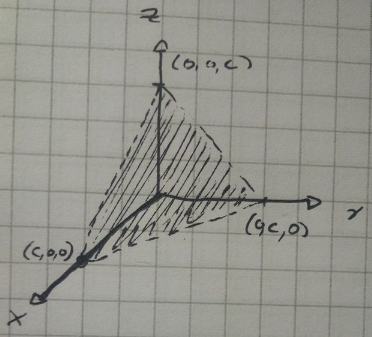
\includegraphics[width=0.5\textwidth]
			{images/esempio3.png}
			\caption{\label{fig:my-label}}}
	\end{figure}	
	
	Calcoliamo i gradienti
	\begin{align}
		{}&\gradient{g}{x,y,z}= (1 \spacecomma 1 \spacecomma 1) \\
		&\gradient{f}{x,y,z}=(yz \spacecomma xz \spacecomma xy)
	\end{align}
	
	Vediamo subito come $g$ non abbia punti di non regolarità, e possiamo quindi applicare Lagrange, dove la prima formulazione della tesi ci porta a scrivere il sistema
	\begin{align}
		\quadruple{yz-xz=0}{xz-xy=0}{yz-xy=0}{x+y+z=c} \implies \quadruple{yz=xz}{xz=xy}{yz=xy}{x+y+z=c}
	\end{align}
	
	Notiamo come la situazione sia un po' intricata.
	
	Se $z=0$ abbiamo che anche $xy=0$ da cui segue che uno dei due deve essere nullo e quindi in automatico anche il rimanente. Ma a noi interessa il massimo, quindi escludiamo valori nulli. Allora avremo
	\begin{align}
		\quadruple{y=x}{z=y}{z=x}{x+y+z=c} \implies x+x+x=3x=c \implies x= \frac{c}{3}
	\end{align}
	
	Abbiamo quindi il nostro punto di massimo in
	\begin{align}
		(x,y,z)_M=\left(\frac{c}{3} \spacecomma \frac{c}{3} \spacecomma \frac{c}{3}\right)
	\end{align}
	
	\newpage
		
	\item Si studi se la funzione
	\begin{align}
		f(x,y,z)=x^2-x +y^2 + z^2 
	\end{align}
	ammette massimo e minimo nel dominio
	\begin{align}
		D = \left\{ x^2 + \frac{y^2}{4}+ \frac{z^2}{9}\leq 1 \right\}
	\end{align}
	
	Studiamo prima i gradienti
	\begin{align}
		{}&\gradient{f}{x,y,z}= \veccolThree{2x-1}{2y}{2z}=\veccolThree{0}{0}{0} \implies \vecx^1=\left(\half \spacecomma 0 \spacecomma 0\right) \\
		&\gradient{g}{x,y,z}= \veccolThree{2x}{\frac{y}{2}}{\frac{2z}{9}} =\veccolThree{0}{0}{0} \implies \vecx^?= \veccolThree{0}{0}{0} \notin \partial D
	\end{align}
	
	Abbiamo quindi un candidato in $\vecx^1$ e nessun punto di non regolarità sulla frontiera per $g$.
	
	Possiamo quindi applicare Lagrange
	\begin{align}
		{}&\triple{Rango \matrixThreeTwo{2x-1}{2y}{2z}{2x}{\half y}{\frac{2}{9}z} =1}{\quad}{g(x,y,z)=0} \nextpassage
		&\quadruple{\frac{y}{2} (2x-1) = 4xy }{ \frac{4}{9} yz = yz  }{\frac{2}{9}yz = yz }{ x^2 + \frac{y^2}{4}+ \frac{z^2}{9}= 1}\implies 
		\quadruple{y(6x+1)=0}{yz=0}{z(16x + 1)=0}{x^2 + \frac{y^2}{4}+ \frac{z^2}{9}= 1}
	\end{align}	
	
	Studiando la seconda equazione del sistema avremo due casi: 
	\begin{enumerate}
		\item $y=0$
		
		In questo caso dalla terza equazione del sistema avremo le seguenti opzioni
		\begin{enumerate}
			\item $z=0$
			Avremo dalla quarta equazione che
			\begin{align}
				x=\pm 1
			\end{align}
			E quindi otteniamo due candidati nei punti
			\begin{align}
				\vecx^{2,3}=(\pm 1 \spacecomma 0 \spacecomma 0)
			\end{align}
			\item $x= -\fracn{16}$
			Sostituendo nell'equazione del vincolo otteniamo
			\begin{align}
				\fracn{16^2} + \frac{z^2}{9}=1 \implies z = \pm \frac{3}{16}\sqrt{255}
			\end{align}
			Abbiamo così ricavato altri due candidati
			\begin{align}
				\vecx^{4,5}= \left( -\fracn{16} \spacecomma 0 \spacecomma  \pm \frac{3}{16}\sqrt{255}  \right)
			\end{align}
		\end{enumerate}
		\newpage
		
		\item $z=0$
		
		In questo caso dalla prima equazione del sistema avremo di nuovo due casi
		\begin{enumerate}
			\item $y=0$
			
			In questo caso riotteniamo i candidati $\vecx^{2,3}$
			
			\item $z=0$
			
			In questo caso otteniamo
			\begin{align}
				x=-\fracn{6}
			\end{align}
			
			Sostituendo nel vincolo otteniamo
			\begin{align}
				\fracn{36} + \frac{y^2}{4}=1 \implies y= \pm \frac{\sqrt{35}}{3}
			\end{align}
			Da cui infine gli ultimi due candidati
			\begin{align}
				\vecx^{6,7}= \left( -\fracn{6} \spacecomma 0 \spacecomma  \pm \frac{\sqrt{35}}{3} \right)
			\end{align}
		\end{enumerate} 
	\end{enumerate}
\end{enumerate}	


Trovati tutti i punti basta calcolare la funzione in tali punti e vedere il più grande e il più piccolo valore assunti.

\newpage

\subsection{Interpretazione geometrica dei moltiplicatori di Lagrange}

Per amor di semplicità affrontiamo il discorso nel piano, ma vale in generale.

Consideriamo una $f(x,y)$con curva di livello
\begin{align}
	\gamma \taleche f(x,y)=f(x_0,y_0)
\end{align}
Con retta tangente in $(x_0,y_0)$
\begin{align}
	r \taleche f_x(x_0,y_0) (x-x_0) + f_y(x_0,y_0)(y-y_0)=0
\end{align}
e sia il vincolo
\begin{align}
	g(x,y)=0 \spacer g(x_0,y_0) =0
\end{align}
con retta tangente in $(x_0,y_0)$
\begin{align}
	\tilde{r} \taleche g_x(x_0,y_0)(x-x_0) + g_y(x_0,y_0)(y-y_0)
\end{align}

Per la seconda formulazione del metodo dei moltiplicatori di lagrange abbiamo che \textbf{le due rette tangenti sono coincidenti, dato che i gradienti delle due funzioni coincidono}.

Questo vuol dire che nei punti di max. e min. la curva di livello corrispondente è tangente al vincolo, e quindi di base si può trattare il problema graficamente, come vediamo nei seguenti \textbf{esempi:}

\begin{enumerate}
	\item $f(x,y)=xy \spacer g(x,y)=x^2 + y^2 -1$
	\begin{figure}[!htb]
		\center{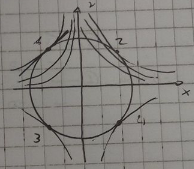
\includegraphics[width=0.3\textwidth]
			{images/IGL1.png}
			\caption{\label{fig:my-label}}}
	\end{figure}	
	Notiamo come graficamente ricaviamo 4 punti critici.
	Se applichiamo lagrange troviamo
	\begin{align}
		{}&\double{\det \matrixTwoTwo{y}{x}{2x}{2y}=0}{x^2 + y^2 =1} \implies \double{x^2 = y^2}{2y^2=1}\nextpassage &\vecx^{1,2,3,4}=(\pm \sqrt{2} \spacecomma\pm \sqrt{2})
	\end{align}
	E quindi abbiamo quattro punti critici anche qui.
	
	\newpage
	\item $f(x,y)=x+y \spacer g(x,y)=x + y^2 -1$
	\begin{figure}[!htb]
		\center{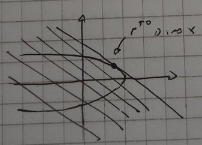
\includegraphics[width=0.3\textwidth]
			{images/IGL2.png}
			\caption{\label{fig:my-label}}}
	\end{figure}
	
	
	In questo caso abbiamo solo un punto di massimo, non essendoci altri punti di tangenza. 
\end{enumerate}

\subsection{Oss. sui punti critici}

\begin{figure}[!htb]
	\center{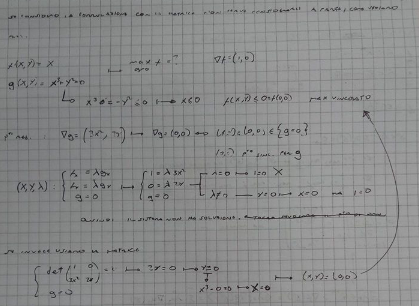
\includegraphics[width=\textwidth]
		{images/soppigro1.png}
		\caption{\label{fig:my-label}}}
\end{figure}

\newpage

\subsection{Metodo dei Moltiplicatori di Lagrange nel caso generale}

\textit{Siano}
\begin{align}
	{}&\deffuncR{n}{} \spacer \deffuncRgen{\vecg}{n}{m} \spacer m<n\\
	&f,\vecg \in C^1(A)
\end{align}
\textit{(Notare come il numero di vincoli deve essere inferiore al numero di variabili.)}

\textit{E sia $\vecx^0 \in A$ tale che}
\begin{enumerate}
	\item $\vecg(\vecx^0)=0$
	\item $\jacobian{g}{\vecx^0}$ \textit{è di rango massimo ($\vecx^0 $ pto regolare per $\vecg$)}
	\item \textit{$\vecx^0 $ punto di ma./min. vincolato di f per $\vecg(\vecx^0)=\veczero_m $}
\end{enumerate}
\textit{Allora avremo di nuovo un risultato esprimibile in tre modi equivalenti:}
\begin{enumerate}
	\item \textit{La matrice}
	\begin{align}
		\veccolFour{\gradient{f}{\vecx^0}}{\gradient{g_1}{\vecx^0}}{\dots}{\gradient{g_m}{\vecx^0}}
	\end{align}
	Sarà di rango massimo.
	\item $\exists \underline{\lambda}^0 \taleche \gradient{f}{\vecx^0} = \braket{\lambda^0 | \gradient{\vecg}{\vecx^0}}=\sum_{j=1}^{m} \lambda^0_j \gradient{g_j}{\vecx^0} $
	\item $\mathcal{L}(\vecx,\underline{\lambda}) = f(\vecx) - \braket{\lambda | \gradient{\vecg}{\vecx^0}} \implies \exists \underline{\lambda}^0 \taleche \gradient{\mathcal{L}}{\vecx^0,\underline{\lambda}^0}=\veczero_n$
\end{enumerate}

Non diamo dimostrazione, ma un paio di esempi operativi nelle prossime pagine.
\newpage
\begin{figure}[!htb]
	\center{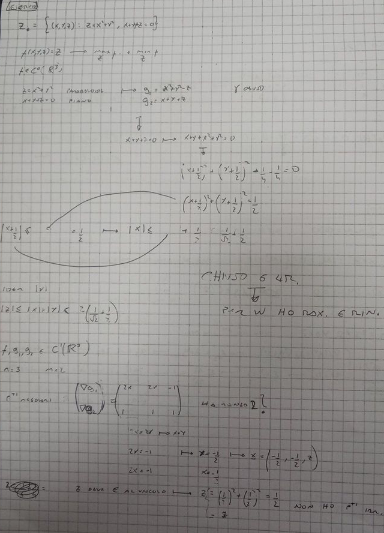
\includegraphics[width=\textwidth]
		{images/esMDL1.png}
		\caption{\label{fig:my-label}}}
\end{figure}

\newpage
\begin{figure}[!htb]
	\center{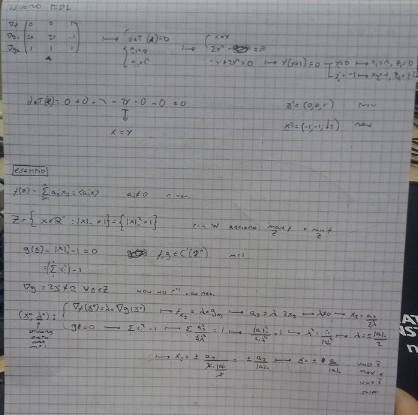
\includegraphics[width=\textwidth]
		{images/esMDL2.png}
		\caption{\label{fig:my-label}}}
\end{figure}

\chapter{Campi conservativi e irrotazionali}

Affronteremo i successivi discorsi in $\R^3$

\section{Richiamo sui campi vettoriali}

Ricordiamo come un campo vettoriale in  sia una funzione del tipo
\begin{align}
	{}&\deffuncRgen{\vecF}{3}{3} \spacer A \text{ aperto}\\
	&\vecF\in C^0(A)
\end{align}

Abbiamo già definito il \textbf{lavoro di un campo vettoriale} come
\begin{align}
	W_{ab}= \int_{\gamma} ds \braket{F|T}= \int_{a}^{b} dt \sum_{i=1}^{3}F_i(x_1(t),x_2(t),x_3(t)) \cdot x'_i(t)
\end{align}

\section{Forme lineari}

Le forme lineari sono un modo alternativo per studiare i campi vettoriali. 

La forma $\omega$ associata al campo $\vecF$ si esprime come
\begin{align}
	\omega = F_1 dx + F_2 dy + F_3 dz
\end{align}

Per le forme lineari vale la proprietà di linearità:
\begin{align}
	{}&\omega_1 = \sum F_i dx_i \spacer \omega_2 = \sum G_i dx_i \spacer \alpha , \beta \in R\\
	&\omega = \alpha \omega_1 + \beta \omega_2 = \sum (\alpha F_i + \beta G_i)dx_i
\end{align}

Le forme lineari possono quindi essere anche viste come
\begin{align}
	\omega = \braket{F|dr}
\end{align}

E quindi si può esprimere il lavoro come
\begin{align}
	W_{ab}=\int_{\gamma} \omega
\end{align}
\newpage
E possiamo quindi riscrivere le proprietà come
\begin{enumerate}
	\item \textbf{Linearità}
	\begin{align}
		\int_\gamma \alpha \omega_1 + \beta \omega_2 =  \alpha \int_\gamma \omega_1 + \beta \int_\gamma \omega_2
	\end{align}
	\item \textbf{Additività sui cammini}
	\begin{align}
		\gamma = \gamma_1 \cup \gamma_2 \spacer \gamma_1 \cap \gamma_2 = \emptyset \implies  \int_\gamma \omega =  \int_{\gamma_1} \omega +  \int_{\gamma_2} \omega
	\end{align}
	\item \textbf{Curve analoghe}
	
	Date $\gamma_1$ e $\gamma_2$ equivalenti si avrà che 
	\begin{enumerate}
		\item con stesso orientamento 
		\begin{align}
			\int_{\gamma_1} \omega =  \int_{\gamma_2} \omega
		\end{align}
		\item con orientamento opposto
		\begin{align}
			\int_{\gamma_1} \omega =  -\int_{\gamma_2} \omega
		\end{align}
	\end{enumerate}
\end{enumerate}

Vediamo un paio di esempi.

\begin{figure}[!htb]
	\center{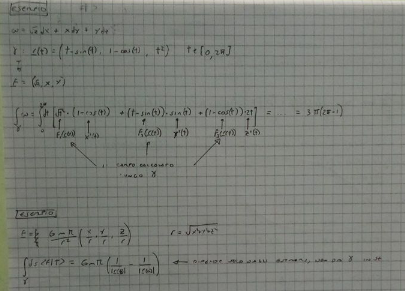
\includegraphics[width=\textwidth]
		{images/esCV1.png}}
\end{figure}

\newpage

\section{Campi conservativi}

Il secondo esempio del paragrafo precedente ci spinge a farci una domanda: quando si ha che il lavoro di un campo vettoriale dipende solo dagli estremi del percorso?

Questo ci porta a dare la definizione di \textbf{campo conservativo}, ovvero un campo $\vecF$ tale che
\begin{align}
	\exists \deffuncRgen{U}{3}{} \spacecomma U\in C^1(A) \spacer \nabla U = \vecF
\end{align}

Con $U$ che prende il nome di \textbf{potenziale} di $\vecF$.

Nel linguaggio delle forme lineari si dice che è una forma $\omega$ è \textbf{esatta} se
\begin{align}
	\exists \; U \taleche \omega = \sum_{i=1}^{3} U_{x_i} dx_i
\end{align}

Ma quanti potenziali può ammettere $\vecF$ in un dominio $A\subset \R^3$ aperto?
\bigskip

Supponiamo di avere due potenziali $U,V$ per $\vecF$. Avremo che in $A$
\begin{align}
	\nabla U = \nabla V \implies \nabla (U-V)=\veczero \implies U-V = cost.
\end{align}

E che quindi tutti i potenziali in $A$ sono uguali a meno di una costante.

Ma in che modo ci sono utili questi potenziali? Lo scopriamo nel seguente \textbf{teorema:}

\bigskip

\textit{Sia $\vecF$ un campo conservativo dotato di potenziale $U$ e sia $\gamma$ curva di estremi $\vecP_i$ e $\vecP_f$, avremo che}
\begin{align}
	\int_{\gamma} ds \braket{F|T}= U(\vecP_f) - U(\vecP_i)
\end{align} 

\bigskip

Per la dimostrazione si procede notando che
\begin{align}
	\dertot{}{t}U(x_1(t) , x_2(t) , x_3(t)) = \sum_{i=1}^{3} U_{x_i} x'_i(t)= \sum_{i=1}^{3} F_i x'_i(t)
\end{align}

E quindi sostituendo nell'integrale del lavoro otteniamo, avendo definito $\vecP_i = \underline{r}(a)$ e $\vecP_f = \underline{r}(b)$
\begin{align}
	\int_{\gamma} ds \braket{F|T} {}&= \int_{a}^{b} dt \sum_{i=1}^{3}F_i(x_1(t),x_2(t),x_3(t)) \cdot x'_i(t) = \continue &=\int_{a}^{b} dt \dertot{}{t}U(x_1(t) , x_2(t) , x_3(t)) = U(\vecP_f) - U(\vecP_i)
\end{align}

\newpage

\subsection{Caratterizzazione dei campi conservativi}

Sia un dominio $A\subset \R^3$ aperto e connesso, e sia un campo vettoriale $\vecF \in C^0(A)$. Avremo che le tre seguenti affermazioni sono equivalenti:
\begin{enumerate}
	\item $\vecF$ è conservativo
	\item $\oint_\gamma ds \braket{F|T}=0 \quad \forall \gamma \text{ chiusa } \subset A$
	\item $\int_{\gamma_1}ds \braket{F|T} = \int_{\gamma_2}ds \braket{F|T}$ date due curve $\gamma_1 \spacecomma \gamma_2$ con stessi estremi ed orientamento
\end{enumerate}

Vediamo come la 1 implichi la 2, dato che utilizzando il teorema dei potenziali e prendendo $\vecP_f=\vecP_i$ otteniamo un integrale chiuso il risultato è nullo.

\bigskip

A sua volta la 2 implica la 3, dato che se due curve hanno gli stessi estremi si avrà che
\begin{figure}[!htb]
	\center{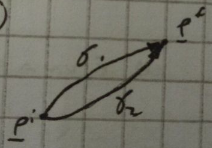
\includegraphics[width=0.3\textwidth]
		{images/cequiv.png}
		\caption{\label{fig:my-label}}}
\end{figure}
\begin{align}
	{}&\gamma = \gamma_1 \cup (-\gamma_2) \text{ curva chiusa}\\
	&\oint_\gamma = \int_{\gamma_1} + \int_{-\gamma_2} = \int_{\gamma_1} - \int_{\gamma_2} \nextpassage
	& \oint_\gamma =0 \implies \int_{\gamma_1} - \int_{\gamma_2} = 0 \implies \int_{\gamma_1} = \int_{\gamma_2}
\end{align}

Infine la 3 implica la 1. Fissato $\vecP^0\in A$ e definita $\Gamma(\vecP) = \gamma_{\vecP^0 \rightarrow\vecP}\subset A$

Dimostriamo come dato 
\begin{align}
	\int_{\Gamma(\vecP)} ds \braket{F|T}=U(\vecP)
\end{align}
$U(\vecP)$ sia un potenziale.

Ci chiediamo
\begin{align}
	\limit{h}{0} \frac{U(x+h,y,z) - U(x,y,z)}{h} \doubteq F_1
\end{align}

\newpage

Iniziamo scomponendo $\Gamma(\vecP^h)$ nel seguente modo
\begin{figure}[!htb]
	\center{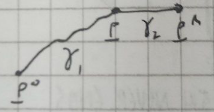
\includegraphics[width=0.3\textwidth]
		{images/cscomp.png}
		\caption{\label{fig:my-label}}}
\end{figure}

\begin{align}
	U(x+h,y,z) = \int_{\Gamma(\vecP^h)} ds \braket{F|T} = \int_{\gamma_1} ds \braket{F|T} + \int_{\gamma_2} ds \braket{F|T}
\end{align}

Il primo integrale è semplicemente $U(x,y,z)$, mentre la curva $\gamma_2$ può essere parametrizzata nel seguente modo
\begin{align}
	\underline{r}(t)= \triple{x(t)=t}{y(t)=y}{z(t)=z} \quad t\in[x,x+h]
\end{align}
Otteniamo così
\begin{align}
	U(x+h,y,z) {}&= U(x,y,z) + \int_{x}^{x+h} dt \; [F_1(x,y,z) \cdot 1 + F_2 \cdot 0 + F_3 \cdot 0]= \continue
	&= U(x,y,z) + \int_{x}^{x+h} dt \; F_1(x,y,z)
\end{align}
Sostituendo nel rapporto incrementale otteniamo
\begin{align}
	U_x(x,y,z) {}&= \limit{h}{0} \fracn{h} \left(  \cancel{U(x,y,z)}  + \int_{x}^{x+h} dt \; F_1(x,y,z) - \cancel{U(x,y,z)} \right) = \continue
	&= \limit{h}{0} \fracn{h} \int_{x}^{x+h} dt \; F_1(x,y,z) = \limit{h}{0} \fracn{h} F_1(x,y,z) \int_{x}^{x+h} dt = \continue
	&= \limit{h}{0} \fracn{h} F_1(x,y,z) h = F_1(x,y,z)
\end{align}
In modo analogo si dimostrano le altre due componenti, e abbiamo così dimostrato che $U(x,y,z)$ è un potenziale, e che quindi $\vecF$ è un campo conservativo. E che per un campo conservativo non importa il tragitto, ma solo gli estremi, dato che $\Gamma(\vecP^h)$ poteva essere parametrizzata in diversi modi ottenendo sempre lo stesso risultato.

\bigskip

Ci chiediamo però: operativamente, come riconosciamo quanto un campo è conservativo? Entra in gioco il \textbf{rotore} del campo $\vecF$:
\begin{align}
	rot \vecF {}&= curl \vecF = \nabla \times \vecF = \det \matrixThreeThree{\hat{i}}{\hat{j}}{\hat{k}}{\partialder{}{x}}{\partialder{}{y}}{\partialder{}{z}}{F_1}{F_2}{F_3}= \continue
	&= \hat{i} \left( \partialder{F_3}{y} - \partialder{F_2}{z} \right)  + \hat{j}  \left( \partialder{F_1}{z} - \partialder{F_3}{x} \right) + \hat{k} \left( \partialder{F_2}{x} - \partialder{F_1}{y} \right)
\end{align}

La matrice è detta \textbf{simbolica} e il determinante è detto \textbf{formale}, perché non rappresentano quantità esistenti ben definite, ma solo "concetti".



Notiamo come se una delle componenti del campo è nulla, e quindi ci troviamo su un piano, il rotore si ridurrà ad una sola componente.

\bigskip

Introduciamo quindi il concetto di \textbf{campo irrotazionale}, ovvero di campo con rotore nullo
\begin{align}
	\nabla \times \vecF = \veczero
\end{align}

Una forma differenziale associata ad un campo irrotazionale viene detta \textbf{chiusa}.

E possiamo quindi dare la \textbf{condizione necessaria di conservatività}:

\bigskip

\textit{Se un campo $\vecF\in C^1(A)$ è conservativo,allora è anche irrotazionale.}

\bigskip

La dimostrazione si appoggia al teorema di Schwartz sulle derivate miste. Infatti essendo $U_{x_i x_j}=U_{x_j x_i}$ si ha che
\begin{align}
	\partialder{F_i}{x_j} = \partialder{F_j}{x_i} \implies \partialder{F_i}{x_j} - \partialder{F_j}{x_i} =0 \quad \forall i,j \implies \nabla \times \vecF=\veczero
\end{align}

\begin{figure}[!htb]
	\center{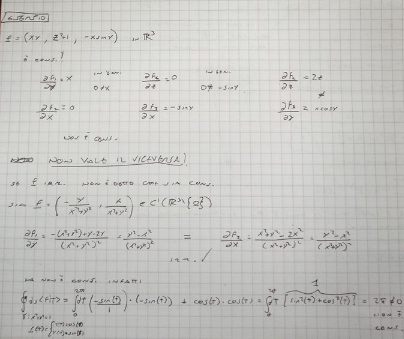
\includegraphics[width=\textwidth]
		{images/cirr.png}}
\end{figure}

\newpage

\section{Domini semplicemente connessi}

Sia $A\subset \R^3$ un dominio aperto e connesso. Avremo che se ogni curva $\gamma\subset A$ chiusa, regolare/a tratti e semplice è frontiera di un insieme $D\subset A$ allora si dice che $A$ è \textbf{semplicemente connesso}.

In altre parole un dominio $A$ è s.c. se ogni $\gamma\subset A$ può essere ridotta con continuità ad un punto senza uscire da $A$.

In $\R^2$ questo significa che un dominio s.c. non ammette buchi al suo interno; cosa che invece cambia per $n\geq 3$, dove se il buco è di un singolo punto il dominio è comunque s.c.

\bigskip

Esempi di insiemi s.c. sono tutti gli insiemi convessi, $\R^2$ e campi circolari, mentre non sono s.c. corone circolari $\R^2 \except{(x_0,y_0)}$ o $\R^3\except{\text{una retta}}$.

\bigskip

I domini semplicemente connessi sono molto comodi da studiare, in quanto portano con loro diversi teoremi utili:

\begin{enumerate}
	\item \textbf{S.C. e convessità}
	
	\textit{Sia $\vecF$ un campo irrotazionale in $A\subset \R^3$}
	
	\textit{Allora se $A$ è s.c. segue che $\vecF$ è convesso in $A$.}
	
	La dimostrazione viene rimandata a quando studieremo il th. di Stokes, in quanto semplifica notevolmente lo studio.
	
	
	\item \textbf{S.C. e conservatività locale}
	
	\textit{Se un campo $\vecF$ è irrotazionale in un dominio aperto $A\subset\R^{2,3}$, allora è anche localmente conservativo in $A$ .}
	
	Avremo quindi dei potenziali \textbf{locali} e che $\exists I(\vecP^0 \in A) \taleche \text{ se } I(\vecP^0) \text{ s.c. } \implies \vecF \text{ cons. }$ e che $I(\vecP^0)=B(\vecP^0,r)$.
	
	\item \textbf{S.C. e conservatività nel piano}	
	
	\textit{Dato un campo vettoriale $\vecF=(F_1(x,y),F_2(x,y))$, se per $(x,y)\in A\subset \R^2$ si ha che $F_{1_x}=F_{2_y}$ allora $\vecF$ è conservativo.}
	
	Diamo in questo caso una dimostrazione del teorema più restrittiva nel prossimo paragrafo, giusto per darci un'idea su come si costruiscano i potenziali.
\end{enumerate}

\newpage

\section{Lemma di Poincarré}

Prima di procedere diamo una definizione utile ai fini di una del seguente teorema:

Un dominio si dice \textbf{stellato rispetto al punto $\vecx^0$} se ogni ogni punto del dominio è collegabile a $\vecx^0$ tramite un segmento.

\textbf{Nota:} un insieme convesso è stellato rispetto ad ogni suo punto. 

\textbf{Nota:} Un dominio stellato è anche s.c., ma un dominio s.c. non è detto sia stellato (e.x. domini a "ferro di cavallo").

\bigskip

Diamo ora il \textbf{Lemma di Poincarré}, il quale ci dice che

\bigskip

\textit{Sia $\vecF$ irrotazionale in un dominio $A$ stellato rispetto ad un punto $\vecP^0$, allora $\vecF$ è anche conservativo.}

\bigskip

Diamo del lemma una dimostrazione costruttiva, ovvero dimostriamo il lemma costruendo un potenziale, e per semplicità ci poniamo in $\R^2$ con $\vecP^0=(0,0)$.

Sia $\gamma=s_{\vecP^0 \rightarrow\vecP}$ il segmento che unisce i punti a $(0,0)$, avremo che
\begin{align}
	\gamma \taleche \underline{r}(t)=\double{x(t)=tx}{y(t)=ty} \quad t\in[0,1]
\end{align}
E dato
\begin{align}
	U(x,y)= \int_{\gamma} ds \braket{F|T}= \int_{0}^{1} dt [F_1(tx,ty) \cdot x + F_2(tx,ty) \cdot y]
\end{align}
Dobbiamo dimostrare che
\begin{align}
	U_x=F_1 \spacer U_y=F_2
\end{align}

Per farlo commettiamo un "abuso" e utilizziamo una nozione, lo scambio tra derivata e integrale, che ancora non sappiamo dimostrare:
\begin{align}
	\partialder{U}{x}{}&= \partialder{}{x} \int_{0}^{1} dt [F_1(tx,ty) \cdot x + F_2(tx,ty) \cdot y] = \continue
	&=\int_{0}^{1} dt \left[\partialder{}{x}(F_1(tx,ty) \cdot x) + \partialder{}{x}(F_2(tx,ty) \cdot y)\right]= \continue
	&= \int_{0}^{1} dt \left[  F_1(tx,ty) + (F_{1_x}(tx,ty)\cdot t)\cdot x +  (F_{2_x}(tx,ty)\cdot t)\cdot y  \right]= \continue
	&= \int_{0}^{1} dt \left[  F_1(tx,ty) + t(F_{1_x}(tx,ty)\cdot x + F_{2_x}(tx,ty)\cdot y)  \right]
\end{align}
Facciamo ora uso dell'irrotazionalità di $\vecF$ e integrando per parti otteniamo
\begin{align}
	\partialder{U}{x}{}&= \int_{0}^{1} dt \left[  F_1(tx,ty) + t(F_{1_x}(tx,ty)\cdot x + F_{2_x}(tx,ty)\cdot y)  \right]= \continue
	&= \int_{0}^{1} dt \left[  F_1(tx,ty) +  \dertot{}{t}F_1(tx,ty)   \right] =\continue
	&= \int_{0}^{1} dt   F_1(tx,ty) +  \int_{0}^{1} dt  \dertot{}{t}F_1(tx,ty) =  \continue
	&= \cancel{\int_{0}^{1} dt F_1(tx,ty)} + tF_1(tx,ty)|_{t=0}^{t=1} - \cancel{\int_{0}^{1} dt F_1(tx,ty)}= \continue
	&= F_1(x,y)
\end{align}
Che è ciò che volevamo. In modo identico si dimostra $U_y= F_2$.

\bigskip

Abbiamo così un pratico criterio per studiare la conservatività di un campo in un dominio:
\begin{enumerate}
	\item $\nabla \times \vecF \doubteq \veczero$
	\item $A$ è s.c. o stellato?
\end{enumerate}

Se la risposta è positiva ad entrambe le domande il campo è conservativo nel dominio $A$.

\chapter{Integrali}

\section{{Integrali a più variabili}}

\subsection{Misura di Peano-Jordan e integrabilità secondo Riemann}

per le funzioni in $\R$ si è definita l'\textbf{integrazione secondo Riemann}, dove bastava che $f(x)$ fosse limitata in un intervallo $[a,b]$ per avere
\begin{align}
	\int_{a}^{b} dx \, f(x)
\end{align}

Riemann può essere esteso ad $\R^2$ tramite la \textbf{misura di Peano-Jordan}. A noi però non interessano, in quanto sono strumenti limitati, come dimostrò Dirichlet con la funzione
\begin{align}
	f(x)=\double{1 \quad x\in [0,1]\cap\Q\quad \;}{0 \quad x\in [0,1], x\notin\Q}
\end{align}
Che non è integrabile in alcun modo con le precedenti definizioni.

Inoltre ci troviamo con le mani legate su molte cose, come lo scambio tra limite e integrale, etc. etc.
Entra quindi in gioco la misura di Lebesgue.

\subsection{Misura di Lebesgue}

\subsubsection{Insiemi misurabili}

La prima domanda che dobbiamo porci è: cos'è un insieme misurabile?

Affrontiamo per semplicità il discorso in $\R^2$, ma le nozioni che verrano date sono estensibili a $\R^n$.

Sia il rettangolo 
\begin{align}
	R= [a_1,b_1]\times [a_2,b_2]
\end{align}

Come sappiamo dalla geometria, una misura sensata della sua area deve dare per forza
\begin{align}
	m(R)=(b_2 - a_2)\cdot(b_1-a_1)
\end{align}

Definiamo ora un \textbf{Plurirettangolo} come l'unione di $n$ rettangoli $R_i$ 
\begin{align}
	P=R_1\cup ... \cup R_n
\end{align}
la cui misura sarà 
\begin{align}
	m(P)= \sum_{i=1}^{n} m(R_i)
\end{align}

Possiamo ora iniziare a studiare domini di forme diverse, usando i Plurirettangoli.

Per esempio dato un insieme aperto $A\neq \emptyset$ possiamo definirne la misura come
\begin{align}
	m(A)=\sup\{ m(P), P\subset A \}
\end{align}

Dato invece un insieme  chiuso $K\neq \emptyset$ possiamo definirne la misura come
\begin{align}
	m(K)=\inf\{ m(P), K\subset P \}
\end{align}

\begin{figure}[!htb]
	\center{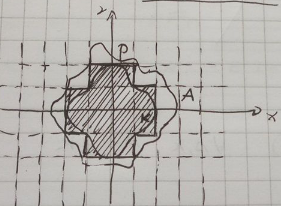
\includegraphics[width=0.5\textwidth]
		{images/insmis.png}
		\caption{Misura in $R^2$}}
\end{figure}

Il caso in $\R^n$ si ottiene generalizzando le formule nel seguente modo:
\begin{align}
	{}&R=[a_1,b_1]\times \dots \times [a_n,b_n]\\
	&m(R)=\prod_{j=1}^{n}(b_j-a_j)\\
	&P= R_1 \cup \dots \cup R_m \spacer R_i \cap R_j = \emptyset \quad \forall i \neq j\\
	&m(P)=\sum_{i=1}^{m}m(R_i)
\end{align}

E le definizioni date per $m(A)$ e $m(K)$ sono identiche a quelle già date.

\newpage

Preso ora un insieme $E \subset \R^n$ possiamo definirne:
\begin{enumerate}
	\item \textbf{Misura esterna:}
	\begin{align}
		\overline{m}(E) = \inf\{m(A), E\subset\underset{aperto}{A}\}
	\end{align} 
	\item \textbf{Misura interna:}
	\begin{align}
		\underline{m}(E) = \sup\{m(K), \underset{chiuso}{K}\subset E\}
	\end{align} 
\end{enumerate}

E affermiamo che $\underline{m}(E) \leq \overline{m}(E)$, dando solo un'idea di dimostrazione:

\bigskip

Se $K \subset E \subset A$ allora $\exists P \taleche K \subset P \subset A$

\bigskip

Questo implica che 
\begin{align}
	m(K)\leq m(P) \leq m(A) \implies m(K)\leq m(A) \quad \forall A,K \taleche K \subset P \subset A
\end{align}

\bigskip

Notiamo ora come preso un dominio aperto $A$ si ha che 
\begin{align}
	{}&m(A)=\overline{m}(A)\\
	&\underline{m}(A)\geq m(P) \quad \forall P \subset A
\end{align}

Ma la seconda equazione ci porta ad avere
\begin{align}
	\underline{m}(A) \geq \sup \{ m(P) \spacecomma \forall P \subset A \} = m(A) \implies \underline{m}(A)\geq m(A)=\overline{m}(A)
\end{align}

Ma per definizione $\overline{m}(A)\geq \underline{m}(A)$ e quindi si ha che
\begin{align}
	\underline{m}(A) =\overline{m}(A) = m(A)
\end{align}

Questo vale non solo per tutti gli aperti $A$, ma anche per i compatti $K$ con procedimento analogo. 

Questo risultato ci tornerà utile nel prossimo paragrafo.

\newpage

\subsubsection{Insiemi misurabili secondo Lebesgue}

Un insieme $E \subset R^n$ si dice misurabile secondo Lebesgue ($L_{mis}$) se
\begin{align}
	{}&\underline{m}(E) =\overline{m}(E) = M  \spacer M= \text{quantità finita}\\
	&m(E)=M
\end{align}

Prendendo in considerazione quanto detto nel paragrafo precente possiamo dire che tutti gli aperti e i compatti sono sempre $L_{mis}$.

Gli insiemi $L_{mis}$ godono delle seguenti proprietà:
\begin{enumerate}
	\item Dati due insiemi $E$ ed $F$ misurabili lo saranno anche 
	\begin{enumerate}
		\item $E\cup F$
		\item $E\cap F$
		\item $E \backslash F$ 
	\end{enumerate}
	\item Sommando i due insiemi si ha $m(E+F)\leq m(E) + m(F)$ e se $E\cap F = \emptyset$ allora $m(E+F)= m(E) + m(F)$
	\item Sommando $n$ domini $E_i$ $L_{mis}$ si ha
	\begin{enumerate}
		\item $	m(E) \leq \sum_{i=1}^{n} m(E_i)$ e si parla di subadditività finita
		\item $m(E) = \sum_{i=1}^{n} m(E_i)$ se $E_i  \cap E_j = \emptyset \quad \forall i,j$ e si parla di additività finita
	\end{enumerate}
\end{enumerate}

\textbf{Nota:} L'insieme degli insiemi misurabili secondo PJ ($PJ_{mis}$) è un sottoinsieme dei $L_{mis}$, in quanto la famiglia di domini integrabili è più restrittiva e si ha
\begin{align}
	{}&\overline{m}_{PJ}(E)=\inf \{ m(\dot{P}), E \subset \dot{P} \} \spacer \dot{P} = \text{plurirett. con punti interni}  \\
	&\underline{m}_{PJ}(E)=\sup \{ m(\dot{P}), \dot{P} \subset E \}
\end{align}

Da cui si ha
\begin{align}
	m\underline{m}_{PJ}(E) \leq \underline{m}_{L}(E) \leq \overline{m}_{L}(E) \leq \overline{m}_{PJ}(E)
\end{align}

E quindi se un insieme è $PJ_{mis}$ è anche $L_mis$.

\begin{figure}[!htb]
	\center{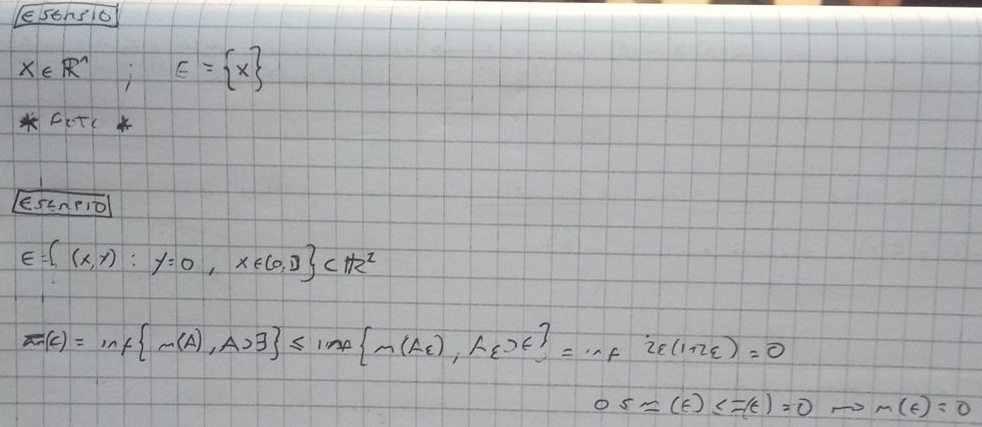
\includegraphics[width=0.8\textwidth]
		{images/insmises.png}
		\caption{\label{fig:my-label}}}
\end{figure}

\newpage

\subsubsection{Teoremi sugli insiemi misurabili}

Diamo ora alcuni teoremi utili ai fini dello studio degli insiemi misurabli.

\begin{enumerate}
	\item \textbf{Teorema dell'additività numerabile della misura}
	
	\textit{Siano $E_1, \dots , E_n$ misurabili, con $E_i \cap E_j =\emptyset \quad \forall i,j$}
	
	\textit{Dato $E= \bigcup_{i=1}^{n} E_i$ se si ha che $\overline{m}(E)< +\infty$ allora}
	
	\textit{E è misurabile e si ha che $m(E)= \sum_{i=1}^{n} m(E_i)$}
	
	\item \textbf{Teorema della subadditività numerabile della misura}
	
	\textit{Siano $E_1, \dots , E_n$ misurabili}
	
	\textit{Dato $E= \bigcup_{i=1}^{n} E_i$ se si ha che $\overline{m}(E)< +\infty$ allora}
	
	\textit{E è misurabile e si ha che $m(E)\leq \sum_{i=1}^{n} m(E_i)$}
	
	\item \textbf{Teorema degli intervalli incapsulati}
	
	\textit{Siano $E_1, \dots , E_n$ misurabili, con $E_1 \subset E_2 \subset \dots \subset E_n$}
	
	\textit{Allora si ha $m(E)= \limit{i}{\infty} m(E_j)$}
\end{enumerate}

\subsubsection{Misurabilità di $\Q\cap [0,1]$ secondo Lebesgue}

Visto che secondo Lebesgue una retta ($ \{ r_j \}$) è un insieme a misura nulla, e dato che
\begin{align}
	\Q \cap [0,1] = \{ r_1, \dots, r_n \} \cdot \{ r_j \}
\end{align}

Si ha che è un insieme a misura nulla.

\subsubsection{Insieme di Cantor}

L'insieme di Cantor viene costruito per ricorrenza nel seguente modo
\begin{align}
	{}&C_0 = [0,1]\\
	&C_1 = C_0 \backslash E_1 \spacer E_1= \left( \frac{1}{3} \spacecomma \frac{2}{3} \right)\\
	&C_2 = C_1 \backslash E_2 \spacer E_2 = \left( \fracn{9} \spacecomma \frac{2}{9} \right) \cup \left( \frac{4}{9} \spacecomma \frac{8}{9} \right)\\
	\vdots
\end{align}

Con
\begin{align}
	\dots \subset C_k \subset C_{k-1}\subset \dots \subset C_0
\end{align}
Da cui si ottiene
\begin{align}
	C= \bigcap_{k=1}^{\infty} C_k = [0,1] \backslash \bigcup_{k=1}^{\infty} E_k
\end{align}

L'insieme di Cantor gode delle seguenti proprietà:
\begin{enumerate}
	\item È un insieme chiuso
	\item $C \neq \emptyset$
	\item non contiene int. (CHE CAZZO VUOL DIRE, CHIEDERE)
	\item Non è numerabile
	\item È misurabile nel seguente modo (si dimostra per induzione)
	\begin{align}
		m(C)= 1 - \sum_{k=1}^{\infty} m(E_k) \spacer m(E_k)= \frac{2^{k-1}}{3^k}
	\end{align} 
\end{enumerate}

\subsubsection{Misurabilità di insiemi chiusi e aperti secondo Lebesgue}

Dato un insieme aperto $E\subset \R^n$, avremo che sarà \Lmis se è misurabile $E\cap B(0,r)$ per ogni $r>0$ e si definisce
\begin{align}
	m(E)= \limit{r}{\infty} m(E\cap B(0,r))
\end{align}

Questo ci permette di poter scrivere
\begin{align}
	\double{\R^n \text{ aperto e misurabile}}{A\subset \R^n \text{ aperto e misurabile}} \implies C= \R^n \backslash A \text{ chiuso e misurabile} \nonumber
\end{align}

\subsubsection{Misura di un prodotto tra spazi}
Dati due spazi $E\subset \R^n$ ed $F\subset \R^k$ a misure rispettivamente $m_n$ ed $m_k$ si ha che dato
\begin{align}
	E \times F = \{ (\vecx,\vecy) , \vecx \in E, \vecy \in F  \}\subset \R^{n+k} \implies m_{n+k}(E\times F) = m_n(E)\times m_k(F)
\end{align}

\section{Integrali di Lebesgue}

Iniziamo il discorso sugli integrali di Lebesgue introducendo le \textbf{funzioni caratteristiche}. Dato un insieme $E\subset \R^n$ avremo
\begin{align}
	\chi_E(\vecx)= \double{1 \quad \vecx\in E}{0 \quad \vecx \notin E}
\end{align}

Avremo che
\begin{align}
	\int_{\R^n} d\vecx \; \chi_E(\vecx)= \int_{\R^n \backslash E} d\vecx \cdot 0 + \int_{E} d\vecx  = m(E)
\end{align}

E possiamo ora definire le \textbf{funzioni semplici} come combinazione lineare di un numero finito di funzioni caratteristiche
\begin{align}
	\Phi(\vecx) = \sum_{j=1}^{n} a_j \chi_{E_j}(\vecx)
\end{align}

Da cui
\begin{align}
	\int_{\R^n} d\vecx  \;  \Phi(\vecx)= \sum_{j=1}^{n} a_j \int_{\R^n} d\vecx  \; \chi_{E_j}(\vecx)=  \sum_{j=1}^{n} a_j m(E_j)
\end{align}

E, prese due funzioni semplici $\Phi$ e $\Psi$ avremo
\begin{enumerate}
	\item \textbf{Linearità:}
	\begin{align}
		\int d \vecx \; [\alpha \Phi(\vecx) + \beta \Psi(\vecx)] = 	 \alpha \int d \vecx \;  \Phi(\vecx) + \beta \int d \vecx \; \Psi(\vecx)  \quad \forall \alpha, \beta
	\end{align}
	\item \textbf{Monotonia:}
	\begin{align}
		\Phi \leq \Psi \implies \int d \vecx \; \Phi(\vecx) \leq \int d \vecx \; \Psi(\vecx)
	\end{align}
\end{enumerate}


Prendiamo ora una generica
\begin{align}
	\deffuncRgen{f(\vecx)}{n}{}
\end{align}
limitata e a supporto compatto, ovvero l'insieme
\begin{align}
	K= \{ \vecx \in A \taleche f(\vecx) \neq 0 \}
\end{align}
è limitato.

Definiamo
\begin{align}
	{}&S_f^+ = \{ \Phi \in S \taleche \Phi(\vecx) \geq f(\vecx) \} \text{ Funzioni semplici maggioranti} \\
	&S_f^- = \{ \Psi \in S \taleche \Psi(\vecx) \leq f(\vecx) \} \text{ Funzioni semplici minoranti} \\
	& S_f^+ \spacecomma S_f^- \neq \emptyset \\
	&|f(\vecx)|\leq M  \implies \double{\Phi(\vecx) = {}&+M \chi_K (\vecx) \in S_f^+}{\Psi(\vecx) = &-M \chi_K (\vecx) \in S_f^-}
\end{align}

Possiamo ora iniziare ad avvicinarci alla definizione di integrale. Infatti ora che abbiamo queste due funzioni possiamo definire
\begin{align}
	{}&\int^+ d\vecx \; f(\vecx)= \inf \left\{ \int d \vecx \; \Phi \spacecomma \Phi \in S_f^+ \right\} \text{ Integrale superiore di  }f(\vecx)\\
	&\int^- d\vecx \; f(\vecx)= \sup \left\{ \int d \vecx \; \Psi \spacecomma \Psi \in S_f^- \right\} \text{ Integrale inferiore di  }f(\vecx)
\end{align}

Si ha che
\begin{align}
	\int^+ d\vecx \; f(\vecx) \geq \int^- d\vecx \; f(\vecx)
\end{align}

E si diche che la funzione è \textbf{integrabile secondo Lebesgue} se

\begin{align}
	\int^+ d\vecx \; f(\vecx) = \int^- d\vecx \; f(\vecx) = \int d\vecx \; f(\vecx)
\end{align}

\textbf{Nota:} Per integrare secondo Riemann ci serviva una classe di funzioni più restrittive, quella delle \textbf{funzioni semplici elementari}, che sono un sotto insieme di quelle necessarie per Lebesgue. Segue quindi che una funzione integrabile per Riemann lo è anche per Lebesgue ma non viceversa.

\newpage

\subsection{Proprietà degli integrali di Lebesgue}

Le proprietà sono le stesse degli integrali di Riemann, ne ricordiamo le più importanti:
\begin{enumerate}
	\item Se una funzione $f$ è sommabile allora lo saranno anche
	\begin{enumerate}
		\item $cf \quad c=costante$
		\item $f^{\pm}= \double{\max\{ f,0\}}{\min\{ -f,0\}}$
		\item $|f|$
		\item $f + a$
	\end{enumerate}
	\item Linearità
	\item Monotonia
\end{enumerate}

\subsection{Funzioni misurabili}

Una funzione
\begin{align}
	\deffuncRgen{f}{n}{*} \spacer \R^* = \R \cup \{ \pm \infty \}
\end{align}

Si dice \textbf{misurabile} se l'insieme
\begin{align}
	F_r = \{\vecx \in \R^n \taleche f(\vecx)>r\}
\end{align}

È misurabile per qualunque $r>0$

\textbf{Nota:} se una funzione è continua è anche misurabile.

Un utilizzo per la definizione di misurabilità si ha nel seguente \textbf{teorema:}

\bigskip

\textit{Data una funzione $\deffuncRgen{f}{n}{}$ questa sarà sommabile \underline{se e solo se } è misurabile.}

\bigskip

Per la dimostrazione iniziamo prendendo un insieme limitato $E\subset\R^n$.

La funzione $f \taleche E \longrightarrow \R$ sarà sommabile in E se lo sarà anche
\begin{align}
	f^*(\vecx)= \double{f(\vecx) \quad {}&\vecx \in E}{0 \quad &\vecx \notin E} = f(\vecx) \cdot \chi_E(\vecx)
\end{align}

Da cui si avrà che
\begin{align}
	\int_E d\vecx \; f(\vecx) = \int_\R d\vecx \; f^*(\vecx)
\end{align}	

Sia ora $f$ non negativa in E, se si ha che

\begin{enumerate}
	\item $f_r(\vecx)= \max (f(\vecx)\spacecomma r)$ è sommabile in $E^*=E \cap B(0,r)$ per ogni $r>0$
	\item Esiste finito $\limit{r}{\infty} \int_{E^*} d\vecx \; f_r(\vecx) $
\end{enumerate} 

Allora anche $f(\vecx)$ è sommabile in $E$.

Se $f$ è a segno qualsiasi si procede nel seguente modo
\begin{align}
	f= f^+ - f^- \spacer \double{f^+ = \max(+f,0)}{f^- = \max(-f,0)} \spacer |f|= f^+ + f^-
\end{align}

Se $f^+$ e $f^-$ sono sommabili allora anche $f$ lo sarà e si avrà
\begin{align}
	\int_E d\vecx \; f = \int_E d\vecx \; f^+ - \int_E d\vecx \; f^-
\end{align}

\textbf{Nota:} Se $f$ è sommabile allora lo sarà anche $|f|$.

Un'ultima considerazione da fare è che $f$ sarà anche integrabile se
\begin{enumerate}
	\item $f_r(\vecx)$ è sommabile
	\item almeno uno tra $f^+$ e $f^-$ è sommabile 
\end{enumerate}

$\pm \infty$ sono soluzioni accettabili per l'integrale

Se vale la prima delle due allora $f(\vecx)$ è anche misurabile. Quindi possiamo riassumere il tutto come segue:
\begin{align}
	\{ f^{ni} \text{ sommabili}  \} \subset \{  f^{ni} \text{ integrabili}  \}  \subset \{  f^{ni} \text{ misurabili}  \}
\end{align}

\begin{figure}[!htb]
	\center{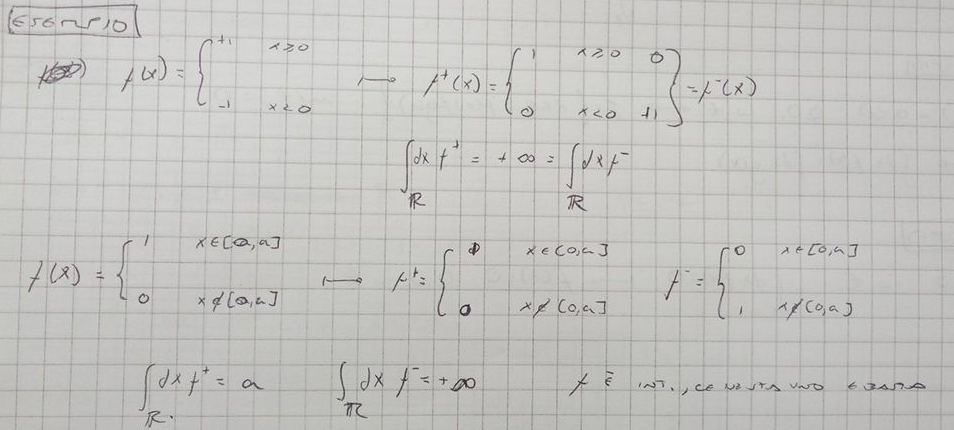
\includegraphics[width=\textwidth]
		{images/fmisintes.png}
		\caption{\label{fig:my-label}}}
\end{figure}


\newpage

\subsection{"Quasi Ovunque"}

Apriamo una brevissima parentesi sul concetto di "Quasi Ovunque", abbreviato \qo (in inglese "Almost Everywhere", A.E.), che ci tornerà utile più avanti.

Si dice che una proprietà è valida \qo in un dominio $A$ se è verificata in tutti i suoi sottoinsiemi tranne quelli a misura nulla.

\begin{figure}[!htb]
	\center{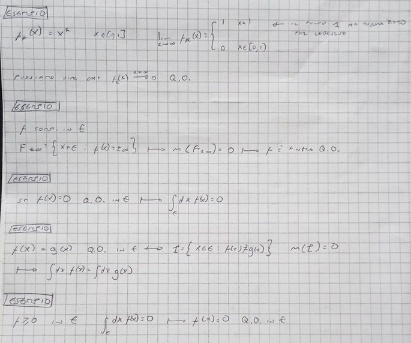
\includegraphics[width=\textwidth]
		{images/qo.png}
		\caption{\label{fig:my-label}}}
\end{figure}

\newpage

\subsection{Criterio del confronto per la sommabilità}

Siano due funzioni
\begin{align}
	f,g \taleche E \subset \R^n \longrightarrow \R
\end{align}

Con $E$ misurabile, e sia che
\begin{enumerate}
	\item $g(\vecx)$ sommabile in $E$, con $g(x)\geq 0$
	\item $f(\vecx)$ misurabile in $E$
\end{enumerate}	

Se $|f(\vecx)|\leq g(x) $ \qo in $E$ allora $f(\vecx)$ è sommabile in $E$.

\subsection{Criterio del confronto asintotico}

Sia $E= [a,b)\subset (-\infty \spacecomma +\infty)$ e siano $f$ e $g$ sommabili in $[a,c]$ con $c<b$ ed esista il limite $\limit{x}{b^-} \frac{f(x)}{g(x)}=l$, avremo allora che
\begin{enumerate}
	\item $l \in (0,+\infty)$
	\begin{align}
		\int_{a}^{b} dx \; f(x) < +\infty \leftrightarrow \int_{a}^{b} dx \; g(x) < +\infty
	\end{align}
	\item $l=0$
	\begin{align}
		\int_{a}^{b} dx \; g(x) < +\infty \implies \int_{a}^{b} dx \; f(x) < +\infty
	\end{align}
	\item $l =+\infty$
	\begin{align}
		\int_{a}^{b} dx \; g(x) = +\infty \implies 	\int_{a}^{b} dx \; f(x) = +\infty
	\end{align}
\end{enumerate}

\begin{figure}[!htb]
	\center{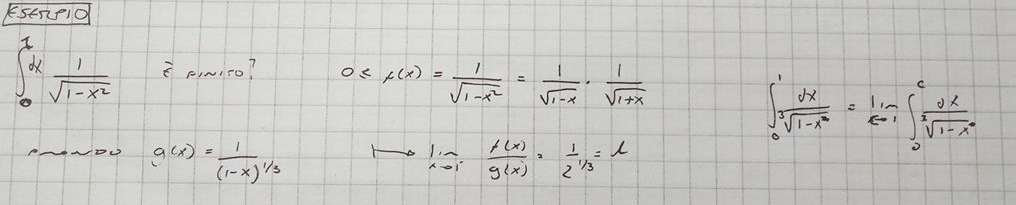
\includegraphics[width=\textwidth]
		{images/confras1.png}
		\caption{\label{fig:my-label}}}
\end{figure}

\begin{figure}[!htb]
	\center{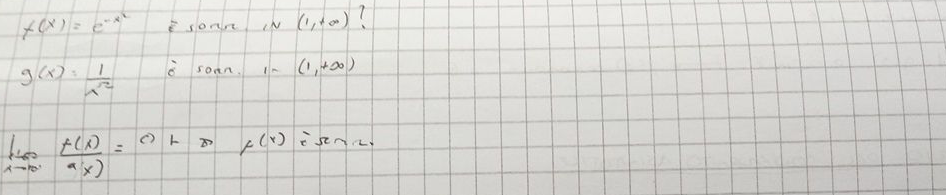
\includegraphics[width=\textwidth]
		{images/confras2.png}
		\caption{\label{fig:my-label}}}
\end{figure}

\subsection{Teorema di passaggio al limite}

Sia la successione di funzioni
\begin{align}
	\{f_n\} \taleche I \subset \R \longrightarrow \R \spacer \{f_n\} \in C^0(I)
\end{align}

Se si ha che $f_n \rightrightarrows f$ in $I$ allora si ha che
\begin{enumerate}
	\item $f\in C^0(I)$
	\item $\int dx \; \limit{n}{\infty}f_n(x)=  \limit{n}{\infty} \int dx \; f_n(x)$ 
\end{enumerate}

Se si ha solo $f_n \longrightarrow f$ il teorema non vale.

\newpage

\subsection{Teorema di convergenza di Poeno-Segre}

Data una successione di funzioni $\{f_n\} \taleche E \subset \R^n \longrightarrow \R$ se vengono rispettate le seguenti condizioni
\begin{enumerate}
	\item $E$ misurabile
	\item $\{f_k(\vecx)\}_{k\geq 1} $
	\item $0\leq f_1(\vecx) \leq f_2(\vecx) \leq \dots \leq f_n(\vecx) $ (la non negatività è opzionale, come vedremo più avanti)
\end{enumerate}

Si avrà che se $f(\vecx)=\limit{k}{\infty}f_k(\vecx)$ allora
\begin{align}
	\limit{k}{\infty} \int_{E} d\vecx \; f_k(\vecx)= \int_{E} d\vecx \; f(\vecx)= \int_{E} d\vecx \;\limit{k}{\infty}  f_k(\vecx)
\end{align}

Perché la non negatività è una condizione opzionale? Perché basta trovare una $g(\vecx)\leq f_1(\vecx)$ e definire
\begin{align}
	F_k(\vecx)= -g(\vecx) + f_k(\vecx)
\end{align}

Che sarà per forza non negativa, e quindi si può applicare il teorema su questa.

\begin{figure}[!htb]
	\center{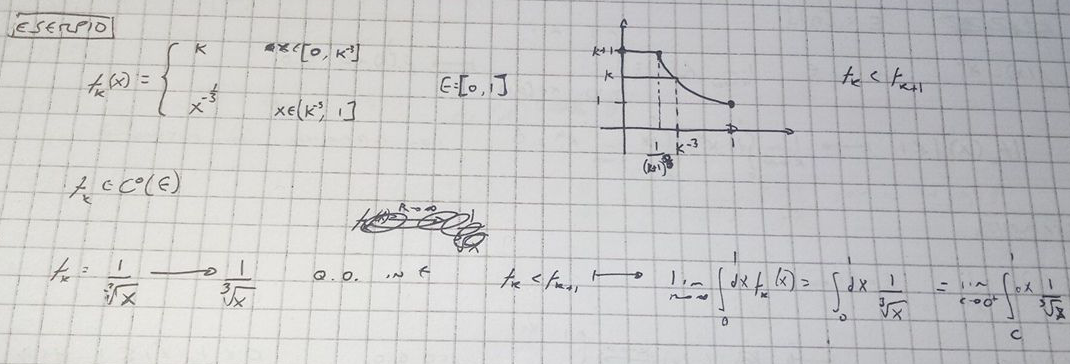
\includegraphics[width=\textwidth]
		{images/conps.png}
		\caption{\label{fig:my-label}}}
\end{figure}

\subsection{Scambio tra somma e integrale per serie a termini non negativi}

Sia una serie
\begin{align}
	\{u_k(\vecx)\}_{k\geq 1} \spacer u_k(\vecx) \geq 0 \quad \forall k \spacecomma \forall \vecx \in E \subset \R^n
\end{align}

E siano $E$ misurabile e gli $u_k$ integrabili in $E$. 

Possiamo definire
\begin{align}
	f_k(\vecx) = \sum_{j=1}^{k} u_j(\vecx) \spacer k \geq 1
\end{align}

Da cui possiamo ricavare
\begin{align}
	f_{k+1} = f_k + u_{k+1} \geq f_k
\end{align}

Il che ci permette di scrivere
\begin{align}
	\limit{k}{\infty} \int_{E} d\vecx \; \sum_{j=1}^{k} u_j(\vecx) = 
	\int_{E} d\vecx \; \limit{k}{\infty}\sum_{j=1}^{k} u_j(\vecx)
\end{align}

Nel termine a sinistra la serie è a termini finiti, e quindi per linearità possiamo invertire serie e integrale e scrivere
\begin{align}
	\limit{k}{\infty}  \sum_{j=1}^{k} \int_{E} d\vecx \; u_j(\vecx) = \sum_{j=1}^{+\infty} \int_{E} d\vecx \; u_j(\vecx) \end{align}

mentre nel secondo termine semplicemente scriviamo
\begin{align}
	\limit{k}{\infty}\sum_{j=1}^{k} u_j(\vecx) = \sum_{j=1}^{+\infty} u_j(\vecx)
\end{align} 

E otteniamo quindi
\begin{align}
	\sum_{j=1}^{+\infty}  \int_{E} d\vecx \;  u_j(\vecx) = \int_{E} d\vecx \; \sum_{j=1}^{+\infty} u_j(\vecx)
\end{align}

\newpage

\subsection{Teorema di Lebesgue per la convergenza dominata}

Se vengono rispettate le seguenti condizioni
\begin{enumerate}
	\item $E\subset \R^n$ misurabile
	\item $\{ f_k(\vecx) \}$ integrabile in $E$ e tale che $\exists f(\vecx)= \limit{k}{\infty} f_k(\vecx)$
	\item $\exists g(\vecx) \geq 0$ sommabile in $E$ tale che $|f_k(\vecx)| \leq g(\vecx)$ \qo in $E$
\end{enumerate}

Allora si ha che
\begin{align}
	\limit{k}{\infty} \int_{E} d\vecx \; f_k(\vecx)= \int_{E} d\vecx \; f(\vecx)= \int_{E} d\vecx \;\limit{k}{\infty}  f_k(\vecx) 
\end{align}

Non dimostriamo il teorema, perché so' conti e non ci serve dimostrarlo.

\bigskip

Rispetto a Poeno-Segre abbiamo l'esistenza di $g(\vecx)$ che domina sia la successione che la funzione a cui tende. Questo ci torna utile qualora ci si trovi a lavorare con una successione limitata. Infatti se $\exists M>0 \taleche |f_k(\vecx)|\leq M$ \qo in $E$ e si ha che $m(E)< + \infty$ possiamo definire
\begin{align}
	g(\vecx)= M \chi_E(\vecx)
\end{align}
E possiamo quindi applicare il teorema di Lebesgue.

\bigskip

Un'altra conseguenza del teorema è che per il teorema del confronto le $f_K(\vecx)$ sono anche sommabili in $E$.

\begin{figure}[!htb]
	\center{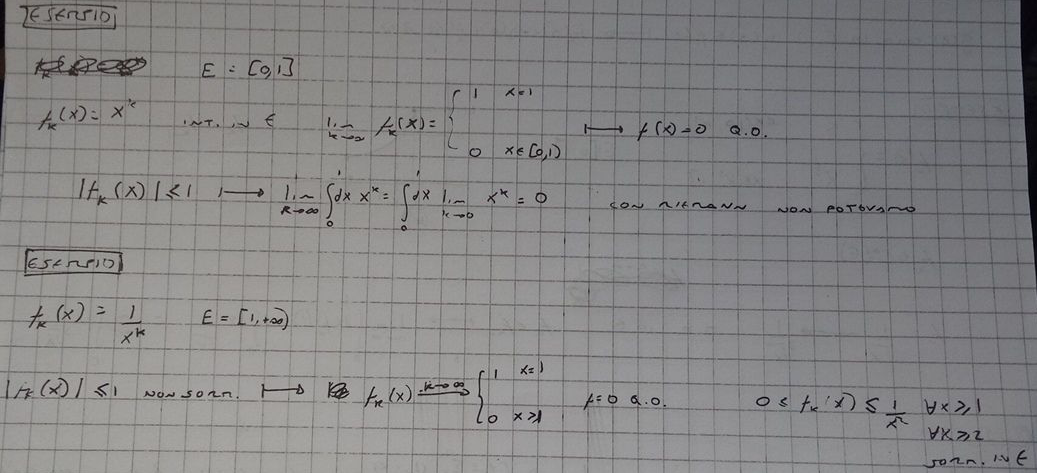
\includegraphics[width=0.9\textwidth]
		{images/convdom.png}
		\caption{\label{fig:my-label}}}
\end{figure}

\newpage


\subsection{Spazi di Lebesgue $L^p$}

Dato un dominio $E\subset \R^n$ misurabile, possiamo definirvi sopra degli spazi $L^p$. Iniziamo col grado più basso, ovvero
\begin{align}
	L^1(E) = \left\{ f \taleche E \subset \R^n \longrightarrow \R \spacecomma \int_{E} d\vecx \; |f(\vecx)|< + \infty  \right\}
\end{align}

$L^1(E)$ è uno spazio normato, con
\begin{align}
	||f||_1 = \int_{E} d\vecx \; |f(\vecx)|
\end{align}

Generalizziamo al caso $L^p$
\begin{align}
	L^p(E) = \left\{ f \taleche E \subset \R^n \longrightarrow \R \spacecomma \int_{E} d\vecx \; |f(\vecx)|^p< + \infty  \right\}
\end{align}

Anche $L^p(E)$ è uno spazio normato, con
\begin{align}
	||f||_p = \left(\int_{E} d\vecx \; |f(\vecx)|^p \right)^{\fracn{p}}
\end{align}

Gli spazi $(L^p \spacecomma ||\cdot||_p)$ sono anche spazi di banach, ovvero normati e completi. 

Inoltre gli elementi dello spazio sono classi di equivalenza rispetto alla relazione $f=g$ \qo in $E$.

\bigskip

Un caso particolarmente interessante si ha per $p=2$, che è anche spazio di Hilbert, dove si ha anche definito il prodotto scalare!
\begin{align}
	||f||_2= \left(\int_{E} d\vecx \; |f(\vecx)|^2 \right)^{\fracn{2}} \spacer \braket{f|g} = \int_{E} d\vecx \; f(\vecx)\cdot g(\vecx)
\end{align}

\subsection{Derivazione sotto segno di integrale}

Prendiamo in considerazione un dominio $E\subset \R^n$ misurabile, un dominio $A=(c,d)\subset \R$ aperto e sia
\begin{align}
	f \taleche E \times A {}& \longrightarrow \R\\
	(\vecx,t) & \longrightarrow f(\vecx,t) \nonumber
\end{align}

Fissiamo $t$ in modo tale che $f(\cdot , t)$ sia integrabile in $A$ e definiamo
\begin{align}
	F(t)= \int_{E} d\vecx \; f(\vecx,t) \spacer t\in A
\end{align}

Ci chiediamo ora. quando è possibile scambiare l'integrale rispetto a $\vecx$ e la derivata rispetto a $t$? 

Innanzitutto dobbiamo assicurarci che $F$ sia continua. Per questo ci viene in aiuto il seguente \textbf{teorema:}

\bigskip

\textit{Se vengono rispettate le seguenti condizioni:}
\begin{enumerate}
	\item $f \taleche \vecx \longrightarrow f(\vecx,t)$ \textit{è sommabile in E $\forall t \in A$}
	\item $f \taleche t \longrightarrow f(\vecx,t)$ \textit{è continua \qo in $A$ $\forall \vecx \in E$}
	\item $\exists g(\vecx)$ \textit{sommabile in $E$ tale che $f(\vecx,t)\leq g(\vecx) \quad \forall t \in A \spacecomma \forall \vecx \in E$ \qo}
\end{enumerate}

\textit{Allora $F(t)$ è continua in $A$.}

\bigskip

Per la dimostrazione, piuttosto che verificare
\begin{align}
	\limit{t}{t_0} F(t) \doubteq F(t_0)
\end{align}

Riscriviamo il problema come
\begin{align}
	\limit{k}{\infty} F(t_k) \doubteq F(t_0) \quad \forall \{ t_k \}_{k\geq 1} \taleche t_k \longrightarrow t_0
\end{align}

Ci troviamo quindi con
\begin{align}
	\limit{k}{\infty} F(t_k) = \limit{k}{\infty} \int_{E} d\vecx \; f(\vecx,t_k)
\end{align}
Grazie alla terza ipotesi possiamo applicare il th. di convergenza dominata, e quindi scrivere
\begin{align}
	\limit{k}{\infty} F(t_k) = \int_{E} d\vecx \; \limit{k}{\infty} f(\vecx,t_k)
\end{align}
Grazie alla seconda ipotesi possiamo scrivere
\begin{align}
	\limit{k}{\infty} f(\vecx,t_k) = f(\vecx,t_0)
\end{align}
E quindi ci troviamo ad avere
\begin{align}
	\limit{k}{\infty} F(t_k) = \int_{E} d\vecx \; f(\vecx,t_0) = F(t_0)
\end{align}
E il teorema è dimostrato.

\bigskip

Ora che ci siamo assicurati di avere fra le mani una funzione continua possiamo enunciare il seguente \textbf{teorema:}

\bigskip

\textit{Se vengono rispettate le seguenti condizioni:}
\begin{enumerate}
	\item $f \taleche \vecx \longrightarrow f(\vecx,t)$ \textit{è sommabile in E $\forall t \in A$}
	\item $f \taleche t \longrightarrow f(\vecx,t)$ \textit{è continua \qo in $A$ $\forall \vecx \in E$}
	\item $\exists g(\vecx)$ \textit{sommabile in $E$ tale che $f(\vecx,t)\leq g(\vecx) \quad \forall t \in A \spacecomma \forall \vecx \in E$ \qo}
	\item $f \taleche t \longrightarrow f(\vecx,t)\in C^1(A) \leftrightarrow f_t(\vecx,t)\in C^0(A)$ 
	\item $\exists g_1(\vecx)$ \textit{sommabile in $E$ tale che $f_t(\vecx,t)\leq g_1(\vecx) \quad \forall t \in A \spacecomma \forall \vecx \in E$ \qo}
\end{enumerate}

\textit{Allora avremo che}
\begin{align}
	F(t)\in C^1(A) \spacer F'(t)= \int_{E} d\vecx \; \partialder{}{t}f(\vecx,t)
\end{align}

\bigskip
Per la dimostrazione procediamo in modo analogo a prima. 

Invece di verificare che
\begin{align}
	\exists \limit{t}{t_0} \frac{F(t) - F(t_0)}{t-t_0} = \text{quantità finita}
\end{align}

Verifichiamo che
\begin{align}
	\exists \limit{k}{\infty} \frac{F(t_k) - F(t_0)}{t_k-t_0} = \text{quantità finita} \quad \forall \{ t_k \}_{k\geq 1} \taleche t_k \longrightarrow t_0
\end{align}

Iniziamo scrivendo il rapporto incrementale
\begin{align}
	\frac{F(t_k) - F(t_0)}{t_k - t_0}
\end{align}

Per linearità possiamo scrivere
\begin{align}
	\frac{F(t_k) - F(t_0)}{t_k - t_0} = \int_{E} d\vecx \; \frac{f(\vecx,t_k) - f(\vecx,t_0)}{t_k - t_0}
\end{align}

Utilizzando il th. di Lagrange avremo
\begin{align}
	\int_{E} d\vecx \; \frac{f(\vecx,t_k) - f(\vecx,t_0)}{t_k - t_0} = \int_{E} d\vecx \; \partialder{}{t}f(\vecx,\xi_k) \spacer \xi_k \in I(t_k,t_0)
\end{align}

Passando a limite, facendo uso del th. della conv. dominata e della continuità della derivata avremo
\begin{align}
	\limit{k}{\infty} \frac{F(t_k) - F(t_0)}{t_k - t_0} {}&= \limit{k}{\infty} \int_{E} d\vecx \; \partialder{}{t}f(\vecx,\xi_k) = \continue
	&= \int_{E} d\vecx \; \limit{k}{\infty} \partialder{}{t}f(\vecx,\xi_k) =  \quad \text{[conv. dominata]}\continue
	&= \int_{E} d\vecx \;  \partialder{}{t}f(\vecx,t_0)  \quad \text{[continuità della der.]}
\end{align}

E il teorema è così dimostrato.

\begin{figure}[!htb]
	\center{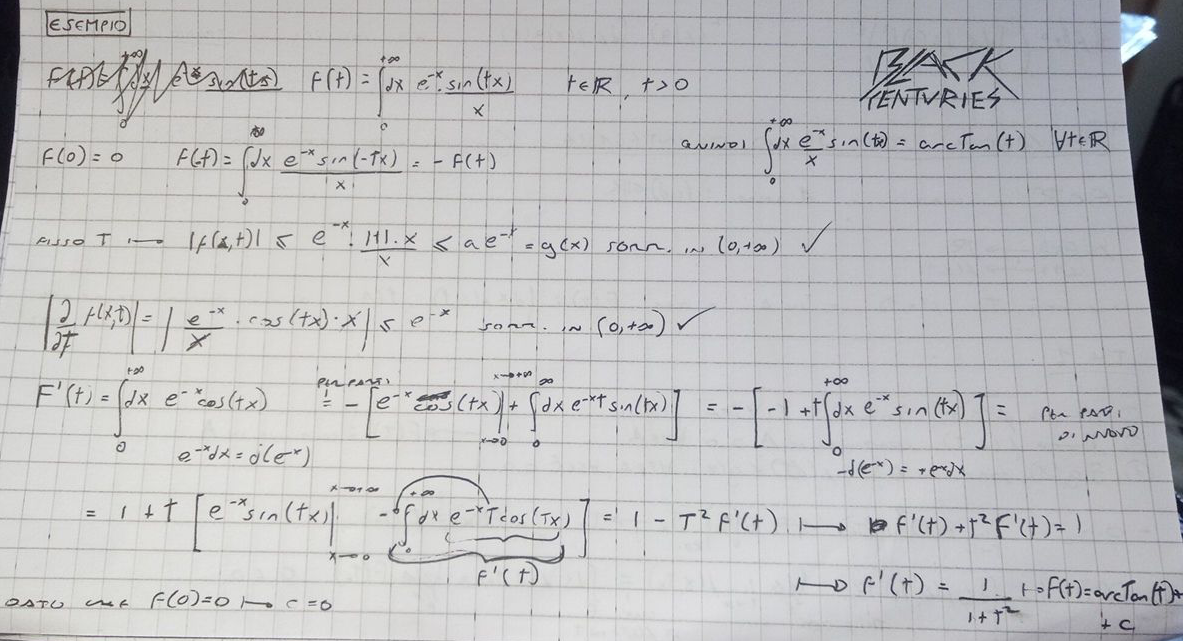
\includegraphics[width=\textwidth]
		{images/derint.png}
		\caption{\label{fig:my-label}}}
\end{figure}
\newpage

FOGLIO 25 BLOCKNOTES NON SI CAPISCE UN CAZZO

\newpage

\subsection{Misura di insiemi in $\R^2$}

Per effettuare la misura di un insieme $E$ in $\R^2$ come quello in figura si può procedere in due modi:

\begin{figure}[!htb]
	\center{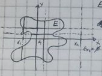
\includegraphics[width=0.3\textwidth]
		{images/misins.png}
		\caption{\label{fig:my-label}}}
\end{figure}

\begin{enumerate}
	\item \textbf{Fissando la $x$}
	\begin{align}
		E_x = \{y \in \R \taleche (x,y)\in E \} \spacer 		m_2(E)= \int_{R}dx \; m_1(E_x) 
	\end{align}
	\item \textbf{Fissando la $y$}
	\begin{align}
		E_y = \{y \in \R \taleche (x,y)\in E \} \spacer m_2(E)= \int_{R}dy \; m_1(E_y) 
	\end{align}
\end{enumerate}

Un insieme si dice
\begin{enumerate}
	\item \textbf{Normale rispetto all'asse $x$} se si ha che
	\begin{align}
		{}&E= \{ (x,y)\in \R^2 \taleche x\in[a,b] \spacecomma y \in [\alpha(x) \spacecomma \beta(x)]   \}\\
		&\alpha(x) \spacecomma \beta(x) \in C^0([a,b]) \spacer \alpha(x) \leq \beta(x) \quad \forall x \in [a,b]
	\end{align}
	\begin{figure}[!htb]
		\center{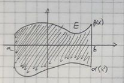
\includegraphics[width=0.3\textwidth]
			{images/misins2.png}
			\caption{\label{fig:my-label}}}
	\end{figure}
	
	In questo caso
	
	\begin{align}
		{}&E_x = \double{\emptyset \quad {}& x \notin [a,b]}{\{  y\in \R \taleche y \in [\alpha(x) \spacecomma \beta(x)]  \} \quad & x \in [a,b]} \\
		& m_1(E_x) = \beta(x) - \alpha(x) \implies m_2(E) = \int_{a}^{b} dx \; [\beta(x) - \alpha(x)]
	\end{align}
	
	
	
	\item \textbf{Normale rispetto all'asse $y$} se si ha che
	\begin{align}
		{}&E= \{ (x,y)\in \R^2 \taleche y\in[c,d] \spacecomma x \in [\gamma(y) \spacecomma \delta(x)]   \}\\
		&\gamma(y) \spacecomma \delta(y) \in C^0([c,d]) \spacer \gamma(y) \leq \delta(y) \quad \forall y \in [c,d]
	\end{align}
	\begin{figure}[!htb]
		\center{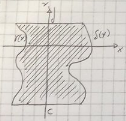
\includegraphics[width=0.3\textwidth]
			{images/misins3.png}
			\caption{\label{fig:my-label}}}
	\end{figure}
	In questo caso
	
	\begin{align}
		{}&E_y = \double{\emptyset \quad {}& y \notin [c,d]}{\{  x\in \R \taleche x \in [\gamma(y) \spacecomma \delta(y)]  \} \quad & y \in [c,d]} \\
		& m_1(E_y) = \delta(y) - \gamma(y) \implies m_2(E) = \int_{c}^{d} dy \; [\delta(y) - \gamma(y)]
	\end{align}
\end{enumerate}

Ovviamente non è detto che se un insieme è normale rispetto ad un asse lo sarà anche rispetto all'altro.

\newpage

ESEMPI SU FOTO SCOMODI DA FOTOGRAFARE, COPIARE POI

\newpage


\subsection{Teorema di Fubini}

Supponiamo di avere una $f(x,y)$ sommabile in $\R^2$. Allora se si ha che
\begin{enumerate}
	\item Fissato $x$ e considerata $f(y)$, essa è sommabile in $\R$.
	
	$f(y) \taleche y \longrightarrow f(x,y)$ è sommabile in $\R$ per $x$ fissato \qo se è ben definito $\int_{R} dy \; f(x,y) = g(x)$  
	
	\item $g(x)$ è sommabile in $\R$ 
\end{enumerate}

Allora si avrà che
\begin{align}
	\iint_{\R^2}dxdy \; f(x,y) = \int_\R dx \; \int_\R dy \; f(x,y)
\end{align}

Oppure, invertendo le variabili nelle ipotesi si avrà
\begin{align}
	\iint_{\R^2}dxdy \; f(x,y) = \int_\R dy \; \int_\R dx \; f(x,y)
\end{align}

\bigskip

Ma c'è un problema! Per come lo abbiamo definito, il teorema non considera domini finiti. E quindi, data una funzione continua definita su $E = \{ (x,y)\in \R^2 \taleche x\in[a,b] \spacecomma y \in [\alpha(x), \beta(x)] \}$, come calcoliamo l'integrale sul dominio? Basta farci furbi e definire
\begin{align}
	f^*(x) = f(x) \cdot \chi_E(x) = \double{f(x) \quad {}& (x,y)\in E }{0 \quad & (x,y) \notin E}
\end{align}

E applicare il th. di Fubini su questa funzione.  Questo ci permette di scrivere
\begin{align}
	{}&\iint_{\R^2}dxdy \; f^*(x,y) = \int_\R dx \; \int_\R dy \; f^*(x,y)\nextpassage
	&\iint_{E}dxdy \; f(x,y) = \int_{a}^{b} dx \; \int_{\alpha(x)}^{\beta(x)} dy \; f(x,y)
\end{align}

\newpage

ESEMPI CHE NON POSSO SCANNARE, DA TRASCRIVERE POI 

\newpage

\subsection{Centro di Massa di una superficie}

Diamo, in modo analogo al caso di una curva, la definizione di baricentro (o CDM) di una superficie $E$ con densità $\rho(x,y)>0$
\begin{align}
	x_B = \frac{\iint_E dxdy \; x\cdot \rho(x,y)}{\iint_E dxdy \;  \rho(x,y)} \spacer y_B = \frac{\iint_E dxdy \; y\cdot \rho(x,y)}{\iint_E dxdy \;  \rho(x,y)}
\end{align}

\begin{figure}[!htb]
	\center{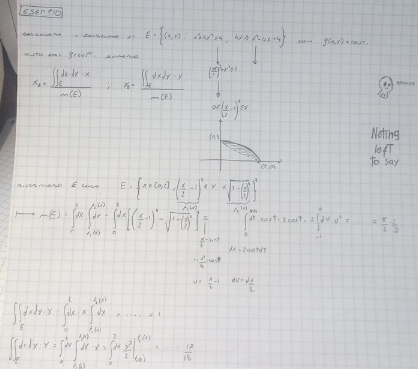
\includegraphics[width=\textwidth]
		{images/cdmsup.png}
		\caption{\label{fig:my-label}}}
\end{figure}

\newpage

\subsection{Calcolo dei volumi}
Dato un insieme $E\subset \R^3$, come troviamo il suo volume?

Fissiamo $z$ in modo tale da avere
\begin{align}
	E_z= \{(x,y) \taleche (x,y,z) \in E\}\subset \R^2
\end{align}

Possiamo procedere come per il caso in $\R^2$, "affettando" il dominio $E$ perpendicolarmente a $z$, e calcolando $m_2(E_z)$, per infine ottenere
\begin{align}
	m_3(E)= \int_{R} dz \; m_2(E_z)
\end{align}

Questo metodo viene chiamato \textbf{Integrazione per strati}.

\begin{figure}[!htb]
	\center{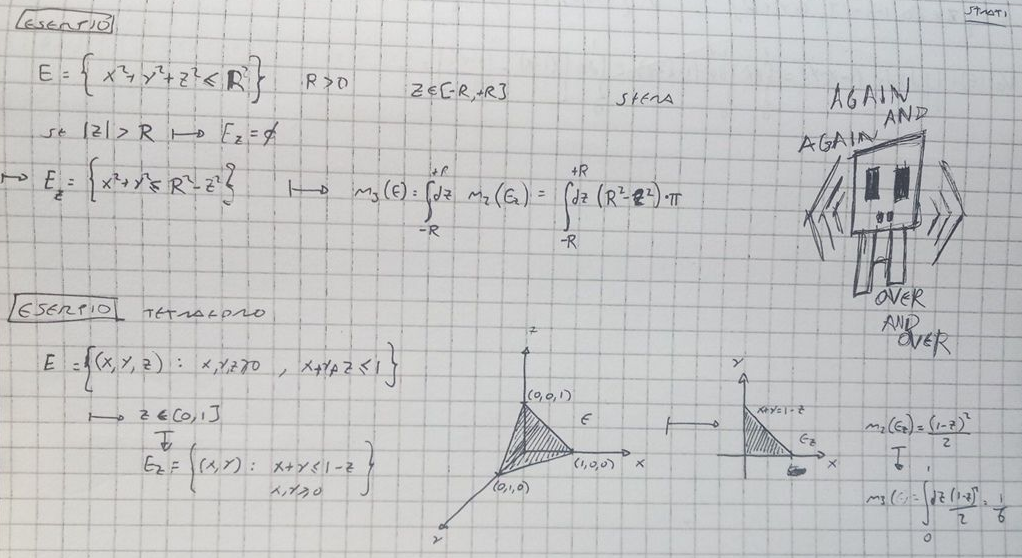
\includegraphics[width=0.6\textwidth]
		{images/intstr.png}
		\caption{\label{fig:my-label}}}
\end{figure}

Alternativamente si può procedere \textbf{per fili}, ovvero dividendo il dominio $E$ nel seguente modo
\begin{align}
	E_{xy} = \{ z \in (x,y,z)\in E \}\subset \R  
\end{align}

Per poi calcolare
\begin{align}
	m_3(E)= \iint_{\R^2} dxdy \; m_1(E_{xy})
\end{align}

\begin{figure}[!htb]
	\center{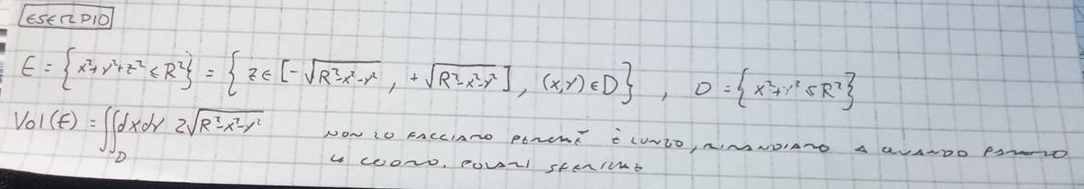
\includegraphics[width=0.7\textwidth]
		{images/intfili.png}
		\caption{\label{fig:my-label}}}
\end{figure}

\subsection{Cambio di variabili (MANCANTE)}

Iniziamo ricordando cos'è un diffeomorfismo. Data
\begin{align}
	g \taleche A \subset \R^n \longrightarrow B \subset \R^n
\end{align}

Con $A$,$B$ aperti. $g$ è un diffeomorfismo se
\begin{enumerate}
	\item $g$ è iniettiva in $A$
	\item															
\end{enumerate}

\newpage

\section{Integrali impropri di Riemann}

Torniamo un attimo agli integrali di Riemann. Gli integrali di Riemann hanno una limitazione: non possono lavorare con intervalli aperti o infiniti. Come si può risolvere questo problema? Utilizzando i limiti.

\subsection{Integrali impropri di Io tipo}

Sia una $f \taleche [a,b) \longrightarrow \R$

Se si ha che
\begin{enumerate}
	\item $f(x)$ è \Rint in $[a,c]$ con $c<b$
	\item Esiste finito $\limit{c}{b^-} \int_{a}^{c} dx \; f(x)$ 
\end{enumerate}

Allora si dice che $f(x)$ è integrabile in senso improprio in $[a,b)$ e si ha che
\begin{align}
	\int_{a}^{b} dx \; f(x)=\limit{c}{b^-} \int_{a}^{c} dx \; f(x)
\end{align}

\begin{figure}[!htb]
	\center{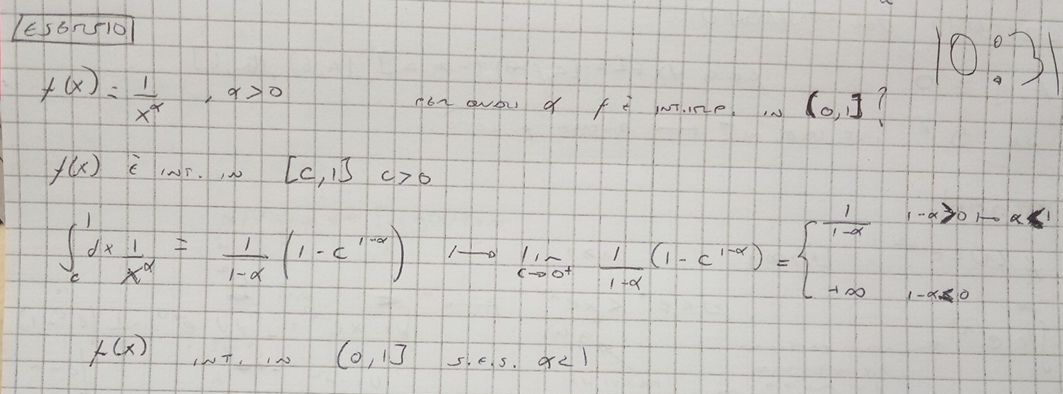
\includegraphics[width=\textwidth]
		{images/intimp1.png}
		\caption{\label{fig:my-label}}}
\end{figure}

\subsection{Integrali impropri di IIo tipo}

Sia ora una $f \taleche [a,+\infty) \longrightarrow \R$

Se si ha che
\begin{enumerate}
	\item $f(x)$ è \Rint in $[a,c]$ con $c>a$
	\item Esiste finito $\limit{c}{\infty} \int_{a}^{c} dx \; f(x)$ 
\end{enumerate}

Allora si dice che $f(x)$ è integrabile in senso improprio in $[a,+\infty)$ 

\begin{figure}[!htb]
	\center{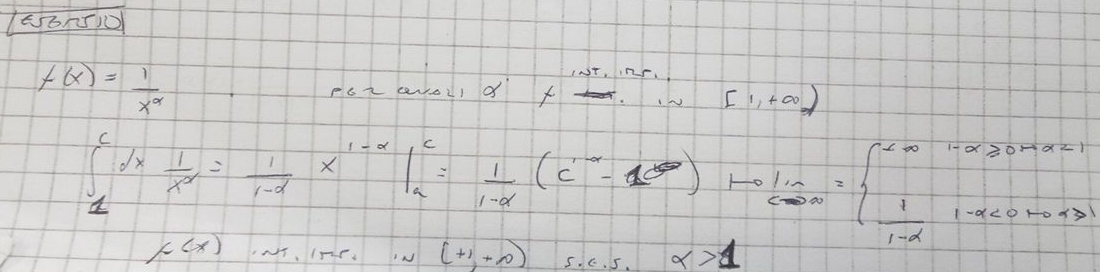
\includegraphics[width=\textwidth]
		{images/intimp2.png}
		\caption{\label{fig:my-label}}}
\end{figure}
\begin{figure}[!htb]
	\center{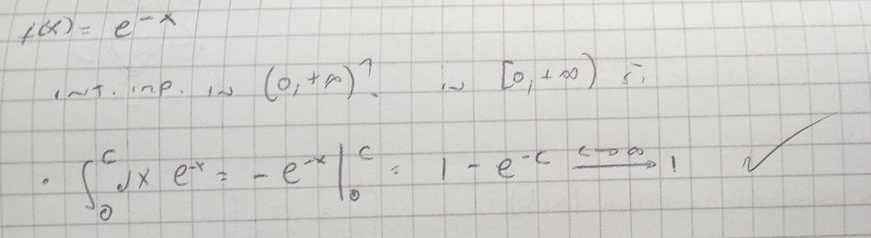
\includegraphics[width=\textwidth]
		{images/intimp3.png}
		\caption{\label{fig:my-label}}}
\end{figure}

\newpage

\subsection{Criterio del confronto per integrali jmpropri}

Siano due funzioni $f,g\geq 0 \taleche f \leq g \quad \forall x \in I=[a, + \infty), (-\infty, +a],[a,b) , (a,b]$  

Se $g$ è integrabile in senso improprio in $I$ allora anche $f$ lo è.

\begin{figure}[!htb]
	\center{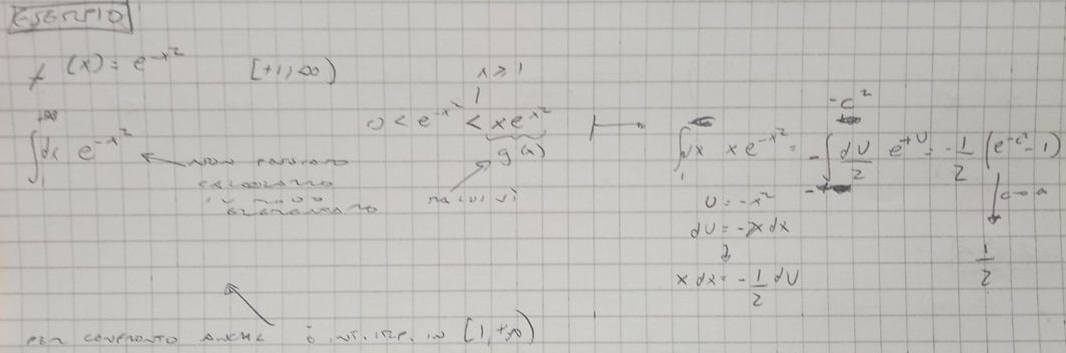
\includegraphics[width=\textwidth]
		{images/intimp4.png}
		\caption{\label{fig:my-label}}}
\end{figure}

\backmatter
% bibliography, glossary and index would go here.

\end{document}